\documentclass{book}

\usepackage[spanish]{babel}
\usepackage[a4paper,top=2cm,bottom=2cm,left=2.5cm,right=2.5cm,marginparwidth=1.75cm]{geometry}

%%-----------------------------------------------
%% Paquetes necesarios
%%-----------------------------------------------
\usepackage{amsmath}
\usepackage{amssymb}
\usepackage{amsthm}
\usepackage{mathtools}
\usepackage{graphicx}
\usepackage{hyperref}
\usepackage{tcolorbox}
\usepackage{listings}
\usepackage{xcolor}
\usepackage{eurosym}
\usepackage{fancyhdr}
\usepackage{float}
\usepackage{subcaption}
\usepackage[utf8]{inputenc}
\usepackage{pdfpages}
\usepackage{tabularx}
\usepackage{array}



\newcommand{\NombreAutor}{Asier Merino Herrán}
\newcommand{\Titulo}{Finanzas cuantitativas}


\title{\Titulo}
\author{\NombreAutor}






%%-----------------------------------------------
%% Definicion de entornos
%%-----------------------------------------------
\newtheorem{remark}{Observación}
\newtheorem{proposition}{Proposición}
\newtheorem{notation}{Notación}

\setcounter{secnumdepth}{3}
\setcounter{tocdepth}{3}


%%-----------------------------------------------
%% Cabeceras y pies de página:
%%-----------------------------------------------
\pagestyle{fancy}
\fancyhf{}
\fancyhead[LO]{\leftmark}
\fancyhead[RE]{\rightmark}
\setlength{\headheight}{1.5\headheight}
\cfoot{\thepage}


%%-----------------------------------------------
%% Páginas en blanco sin cabecera:
%%-----------------------------------------------
\makeatletter%
\addto\shorthandsspanish{\let\esperiod\es@period@code}%
\def\clearpage{%
  \ifvmode%
    \ifnum\@dbltopnum=\m@ne%
      \ifdim\pagetotal<\topskip%
        \hbox{}%
      \fi%
    \fi%
  \fi%
  \newpage%
  \thispagestyle{empty}%
  \write\m@ne{}%
  \vbox{}%
  \penalty-\@Mi%
}%
\makeatother



\begin{document}

  \begin{titlepage}
      \centering
      \vspace{3cm}
      {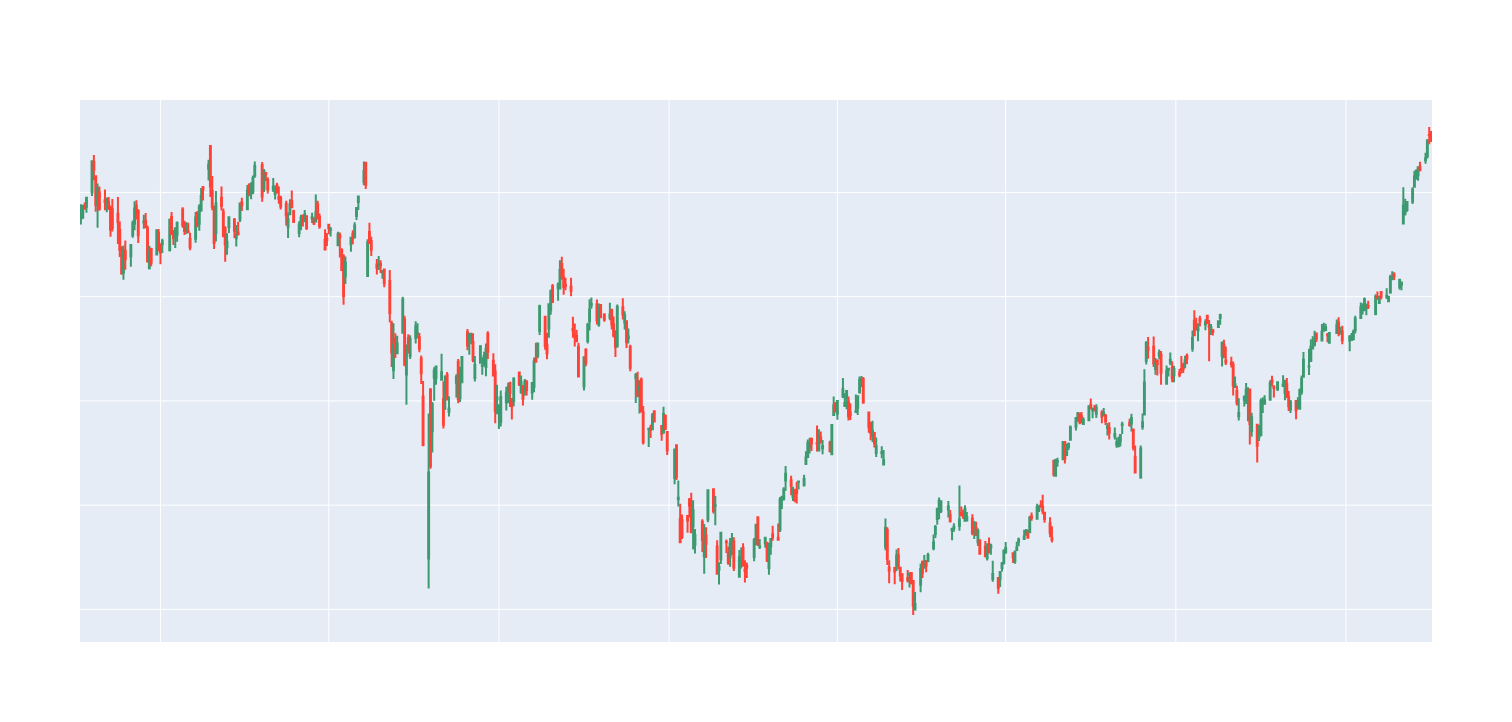
\includegraphics[width=0.9\textwidth]{newplot.png}\par}
      \vspace{5cm}
      {\scshape\Huge \Titulo\par}
      \vspace{2cm}
      {\scshape\LARGE Apuntes-esquema \par}
      \vfill
      {\Large Autor:  \par}
      {\Large \NombreAutor\par}
      \vfill
      {\Large \today \par}
  \end{titlepage}


  \clearpage%
  \tableofcontents
  \setcounter{page}{1}
  \pagenumbering{arabic}


  %PRIMERA PARTE: FUNDAMENTOS BÁSICOS DE DERIVADOS, RIESGO Y RENTABILIDAD
  \clearpage%
  \part{Fundamentos básicos de derivados, riesgo y rentabilidad}
  \chapter{Introducción}
  \section{Conceptos financieros básicos}
En esta sección se explican ciertos conceptos financieros básicos en inglés.

\subsection{Terminología básica}\label{sec:terminos_basicos}
\begin{itemize}
    \item \textbf{Equity, stock, share}: acción de una empresa.
    \item \textbf{Shareholders}: accionistas.
    \item \textbf{Dividens}: dividendos. Pagas generalmente cada 6 meses. \textbf{Cum} cuando se va a pagar el siguiente dividendo o \textbf{Es} cuando no. Suele haber bajadas del precio de acción cuando se paga dividendo. Si en cierto momento $t_d$ se paga un dividendo $q\cdot S$, justo después de pagar el dividendo la acción en ausencia de arbitraje vale 
    \[S(1-q)\]
    \item \textbf{Stock split}: De vez en cuando empresas pueden hacer división de acciones, i.e, cada acción pasa a ser $N$ acciones y el precio se divide entre $N$.
    \item \textbf{Commodities}: producto en bruto como oro, petróleo, \dots Se suelen usar en mercados a futuro.
    \item \textbf{Foreign exchange, Forex, FX}: Cambio de divisas. Debe haber cambio consistente entre divisas para evitar arbitraje.
    \item \textbf{Índice}: Medida de cómo va un mercado/economía. Se calcula como la suma de un \textbf{basket} o conjunto selecto de acciones.
    \item \textbf{Interest}:
    \begin{itemize}
        \item \textbf{Simple interest}: se aplica interés $r$ al valor inicial.
        \[(1+r)P\]
        \item \textbf{Compound interest}: se aplica interés $r$ al valor inicial y al interés ganado:
        \begin{itemize}
            \item \textbf{Discretely compounded interest}:
            \[\left(1 +\frac{r}{m} \right)^{mn}P\]
            \item \textbf{Continuously compounded interest}:
            \[\lim_{m\rightarrow\infty}\left( 1+\frac{r}{m} \right)^{mn}P=e^{nr}P\]
        \end{itemize}
        \item \textbf{Fixed}: interés fijo.
        \item \textbf{Floating}: interés variable.
    \end{itemize}
    \item \textbf{Present value}: actualización de un valor futuro. 
    \item \textbf{Coupon-bearing bonds}: bonos con cupón cada X tiempo que finalmente paga un \textbf{principal}.
    \item \textbf{Interest rate swaps}: dos partes se intercambian los intereses, por ejemplo, uno paga un $r$ fijo y el otro el del Euribor 6M, o Euribor 3M vs Euribor 6M. Hay un capítulo entero a continuación.
    \item \textbf{Index-linked bond}: bonos asociados a un índice para evitar la inflación.
    \item \textbf{Retail Price Index (RPI)}: índice que mide la inflación en el Reino Unido.
    \item \textbf{Consumer Price Index (CPI)}: índice que mide la inflación en EE.UU.\@
    \item \textbf{Short position}: vender un activo (esperando que baje de precio).
    \item \textbf{Long position}: comprar un activo (esperando que suba de precio).
    \item \textbf{Derivatives}: instrumento financiero cuyo valor depende del valor de otro activo.
    \item \textbf{Close position}: terminar una inversión o apuesta que se había abierto anteriormente, p.e.\ vender/comprar algo, dejar que algo expire, ejercer un contrato, \ldots{}
    \item \textbf{Fundamental analysis}: determinar el valor intrínseco o correcto de una empresa estudiando sus balances contables, estados financieros, equipo de gestión, patentes, competencias, proyecciones de beneficios, flujos de caja, \dots Es muy complejo y hay veces en las que el mercado se comporta de manera irracional.
    \item \textbf{Technical analysis}: no importa lo que hace la empresa, se analiza cómo se comporta la acción usando gráficos de precios, tendencias, patrones técnicos, \dots Se considera una pseudo-ciencia.
    \item \textbf{Quantitative analysis}: enfoque matemático y estadístico de los mercados financieros. Se usa para valorar derivados, gestión de riesgos, teoría de carteras, \dots
    \item \textbf{Return}: porcentaje de crecimiento.
\end{itemize}


\subsection{Contratos forward y futures}
\begin{itemize}
    \item \textbf{Forward contract}: una parte se compromete (y se \textbf{obliga}) a comprarle un activo a otra parte en la \textbf{delivery date} o \textbf{maturity} del contrato por un \textbf{delivery price}. EL \textbf{forward price} es el precio actualizado del subyacente (teniendo en cuenta interés, cupones, etc para que el contrato tenga valor inicial del contrato sea 0). El forward price cambia en cada momento, pero el delivery price se fija al firmar el contrato.
    \item \textbf{Future cotract}: como el forward, pero más público, estandarizado, con un ajuste diario y menor flexibilidad. Por ejemplo, un trader especulando con el SP500.
    \item \textbf{Spot price}: el valor de activo subyacente en tiempo $t$, i.e., $S_t$.
    \item \textbf{Going short}: vender un activo que no tienes, con la promesa de recomprarlo más adelante para devolverlo.
\end{itemize}
Para que uno de estos contratos no tenga arbitraje se debe cumplir que
\[S(t)e^{r(T-t)}-F=0 \Rightarrow F=S(t)e^{r(T-t)}\]



\subsection{Contratos future}
Siempre hay un \textbf{delivery and Settlement} en el que se debe entregar el subyacente, pero muchas veces el contrato se cierra antes o se liquida en efectivo la diferencia entre lo pactado y el valor actual.
Al entrar en futuros, debe haber un depósito de dinero (\textbf{Margin}) como garantía de que vas a pagar. Según va cambiando día a día el precio del contrato, se va añadiendo o retirando dinero de tu \textbf{margin account}. Como se da esta compensación diaria (cada dia me pagan/pago lo que haya ganado/perdido segun lo que firmé), el valor del contrato de resetea a 0 todos los días.
\begin{itemize}
    \item \textbf{Initial Margin}: fianza inicial al abrir posición.
    \item \textbf{Maintenance Margin}: mínimo que debe haber en la cuenta.
\end{itemize}

\subsubsection{Commodity futures}
Futuros sobre materias primas, entra en juego costo de almacenamiento y rendimiento de conveniencia.
\[F=S(t)e^{(r+s-c)(T-t)}\]
donde $s$ es el \textbf{storage cost} y $c$ es el \textbf{convenience yield}, que es el beneficio de tener el bien físicamente.
\begin{itemize}
    \item \textbf{Backwardation}: cuando el storage cost domina sobre el convenience yield
    \[F=S(t)e^{(r+s-c)(T-t)}<S(t)e^{r(T-t)}\]
    \item \textbf{Contango}: cuando el convenience yield domina sobre el storage cost. SObre todo cuando el bien es escaso
    \[F=S(t)e^{(r+s-c)(T-t)}>S(t)e^{r(T-t)}\]
\end{itemize}


\subsubsection{FX futures}
Contrato para comprar o vender divisas. No hay costes de almacenamiento, pero la divisa extranjera genera intereses si se invierte en banco extranjero.
\[F=S(t)e^{(r-r_f)(T-t)}\]
donde $r$ es interés doméstico y $r_f$ es interés extranjero.


\subsubsection{Index futures}
Futuros sobre índices de acciones. Similar a los FX, los dividendos bajan el valor del futuro.
\[F=S(t)e^{(r-q)(T-t)}\]
donde $q$ es el porcentaje anual de dividendo.






\subsection{Conteo de días}
Algunas maneras de contar los días entre dos fechas:
\begin{itemize}
    \item \textbf{Actual/Actual}: número de días normal que hay en el calendario.
    \item \textbf{30/360}: cada mes tiene 30 días y el año tiene 360 días
    \item \textbf{Actual/360}: cada mes tiene los días que toca, pero el año tiene 360 días.
\end{itemize}





  \clearpage%
  \chapter{Productos financieros básicos}
  

\section{Opciones}
Una \textbf{Call} option es el derecho a comprar un \textbf{underlying asset} por un \textbf{exercise/strike price} hasta o el \textbf{expiry/expiration date}.\ Una \textbf{put option} es lo mismo, pero te da derecho a vender. Muchas veces las opciones se agrupan en \textbf{series}, i.e.\ diferentes combinaciones de strike y vencimiento disponibles para un mismo activo. Su \textbf{payoff function} es:
\begin{itemize}
    \item \textbf{Call option}: Apuestas a que el mercado sube
    \[\boxed{\max(S-K, 0)}\]
    \begin{figure}[H]
        \centering
        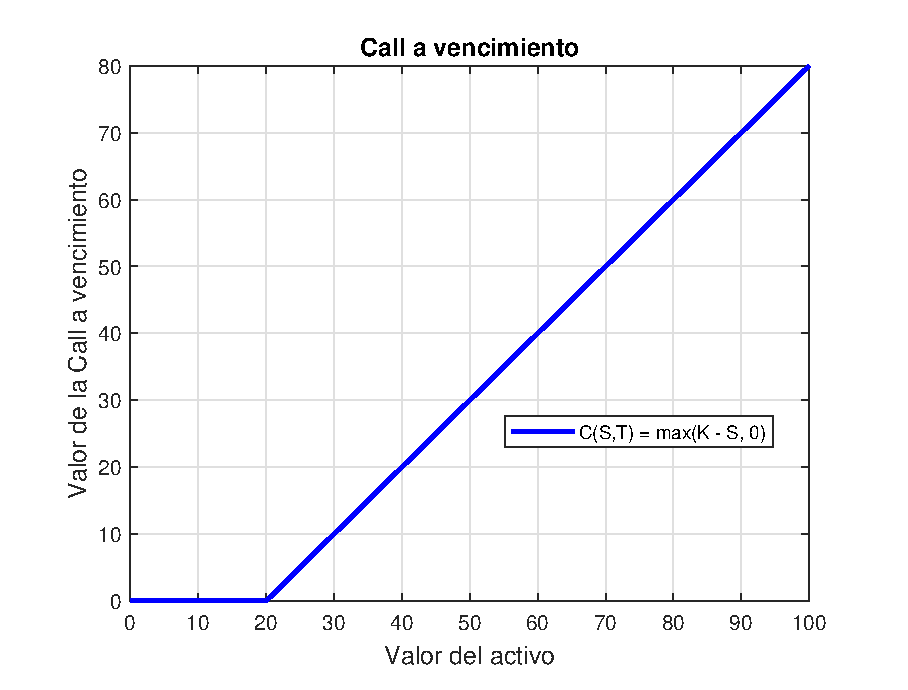
\includegraphics[width=0.5\linewidth]{Imagenes/Parte1/2_Derivados/PayOffCall.eps}
        \caption{Payoff de opción Call a vencimiento}
    \end{figure}
    \item \textbf{Put option}: Apuestas a que el mercado baje
    \[\boxed{\max(K-S, 0)}\]
    \begin{figure}[H]
        \centering
        \includegraphics[width=0.5\linewidth]{Imagenes/Parte1/2_Derivados/PayOffPut.eps}
        \caption{Payoff de opción Put a vencimiento}
    \end{figure}
\end{itemize}
A veces el strike $K$ se representa con una $E$. Las opciones \textbf{vainilla} son aquellas más simples; la función de pago solo depende del valor del subyacente en el momento del pago. Los \textbf{derivatives or contingent claims} son contratos que tienen dependencias más complejas.


\subsection{Terminología}
\begin{itemize}
    \item \textbf{Premium}: lo que se paga inicialmente por el contrato (prima).
    \item \textbf{Underlying (asset)}: subyacente sobre el que depende el contrato.
    \item \textbf{Strike (price)/exercise price}: precio al que se compra o vende el subyacente. Se define con $E$ o con $K$.
    \item \textbf{Expiration (date) o expiry (date)}: fecha en la que se puede ejercer o cuando se caduca la opción. Se denota por $T$.
    \item \textbf{Intrinsic value}: Valor del beneficio si la opción se ejerce en ese momento.
    \item \textbf{Time value}: Valor extra que tiene la opción por la incertidumbre futura.
    \item \textbf{In the money}: Opción con valor intrínseco positivo. Call: precio activo $>$ strike. Put: precio activo $<$ strike.
    \item \textbf{Out of the money}: Opción sin valor intrínseco. Call: precio activo $<$ strike. Put: precio activo $>$ strike.
    \item \textbf{At the money}: Precio del activo $\approx$ strike.
    \item \textbf{Long position}: Posición positiva en una cantidad o exposición.
    \item \textbf{Short position}: Posición negativa o venta en corto de un activo. ``Vender sin tener activo para adelantar dinero''.
    \item \textbf{Profit diagram}: Como el payoff, pero restandole la prima.
    \begin{figure}[H]
        \centering
        \begin{subfigure}[b]{0.45\linewidth}
            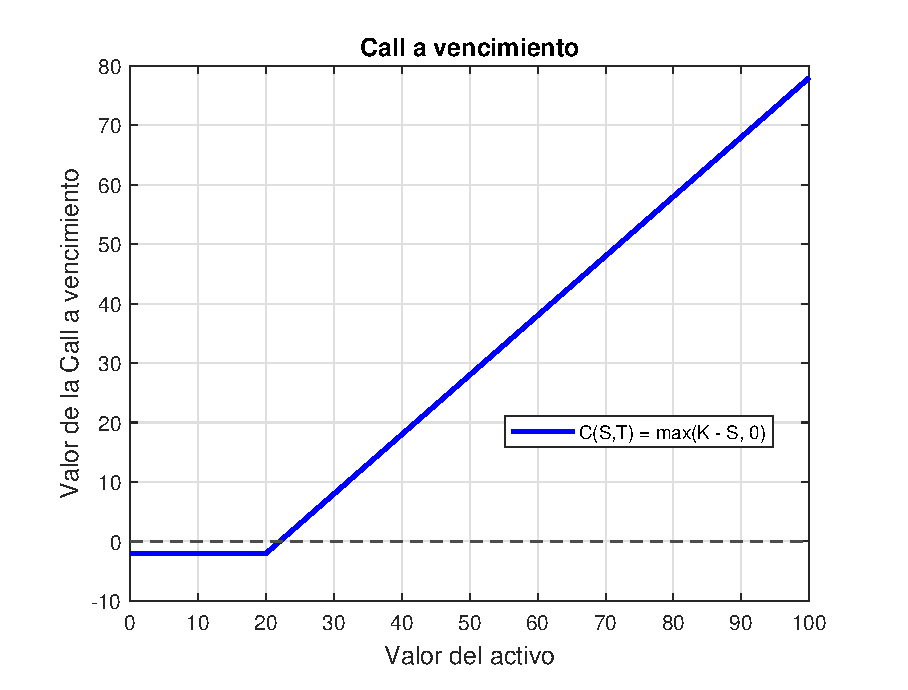
\includegraphics[width=\linewidth]{Imagenes/Parte1/2_Derivados/ProfitDiagCall.eps}
            \caption{Call option}
        \end{subfigure}
            \begin{subfigure}[b]{0.45\linewidth}
            \includegraphics[width=\linewidth]{Imagenes/Parte1/2_Derivados/ProfitDiagPut.eps}
            \caption{Put option}
        \end{subfigure}
        \caption{Profit diagram de opción a vencimiento}
    \end{figure}
    \item \textbf{Over the counter/OTC}: opciones que se realizan fuera de la bolsa y que no tienen que seguir las convenciones estándar. Los términos se especifican en una \textbf{term sheet}.
    \item \textbf{Gearing/leverage}: relación entre la posible ganancia y la inversión. Las opciones tienen una gran gearing, pero el punto negativo es que si no hay ganancias, la pérdida es del 100\% (se pierde la prima). Aquí el writer es el que tiene mucho riesgo.
    \item \textbf{Hedging}: tomar posiciones contrarias, por ejemplo ser el writer de una opción y comprar/vender acciones del subyacente para reducir riesgos. También se usa para describir la reducción de la aleatoriedad en general.
\end{itemize}



\subsection{Tipos de opciones}
\begin{itemize}
    \item \textbf{European options}: solo se puede ejercer en vencimiento.
    \item \textbf{American options}: se puede ejercer en cualquier momento hasta el vencimiento.
    \item \textbf{Bermudan options}: se puede ejercer en ciertas fechas específicas.
\end{itemize}


\subsection{Call-Put Parity}
La relación en cualquier tiempo $t$ entre una Call y una Put con los mismos parámetros es:
\[
    \boxed{C-P=S-Ke^{-r(T-t)}}
\]



\subsection{Opciones binarias/ digitales}
A fecha de ejercicio son discontinuas. Pagan una cierta cantidad fija (como un \$1) si el subyacente está por encima/debajo de cierto precio de ejercicio $E$ (o $K$). Las vainilla tienen un potencial de ganancia ilimitado, mientras que las binarias están acotadas, porque las compras cuando crees que el crecimiento/bajada es limitado.
\begin{figure}[H]
    \centering
    \begin{subfigure}[b]{0.45\linewidth}
        \includegraphics[width=\linewidth]{Imagenes/Parte1/2_Derivados/BinaryCall.eps}
        \caption{Call option}
    \end{subfigure}
        \begin{subfigure}[b]{0.45\linewidth}
        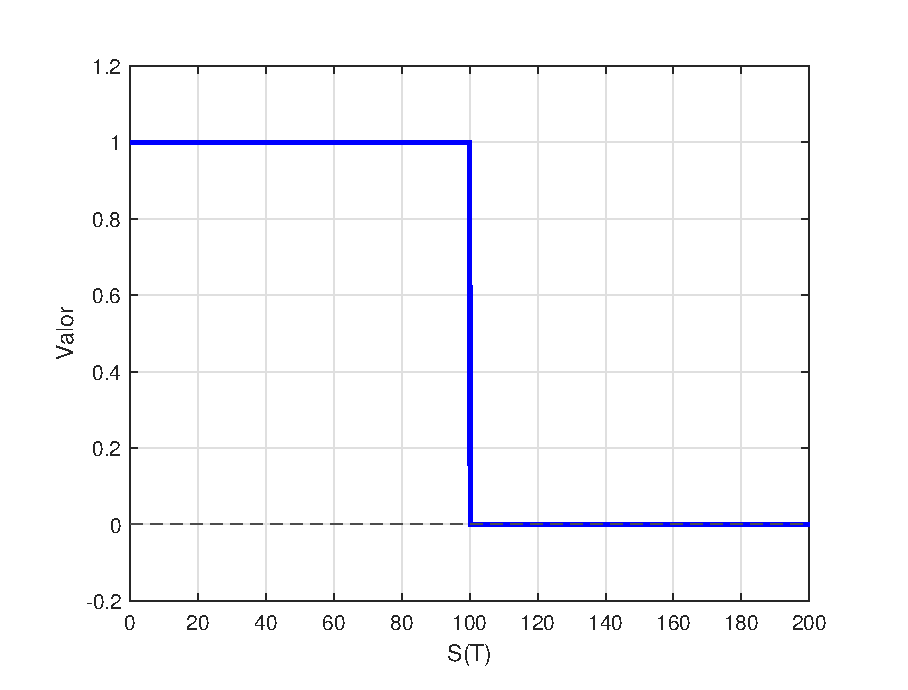
\includegraphics[width=\linewidth]{Imagenes/Parte1/2_Derivados/BinaryPut.eps}
        \caption{Put option}
    \end{subfigure}
    \caption{Binary option payoff}
\end{figure}
Su relación de paridad se obtiene considerando que tienes una opción binary de cada tipo, porque a precio de ejercicio se obtiene el \$1 que se paga (o la cantidad que se haya firmado) actualizado:
\[\text{Binary call} + \text{Binary put} = e^{-r(T-t)}\]




\subsection{Portfolio of options/Option strategy}
Conjunto de opciones combinadas de manera estratégica para un objetivo concreto (maximizar ganancias, minimizar riesgos,\dots). Para saber su payoff se suman los payoff de las opciones que compras y se restan los payoff de las opciones que vendes. De forma genérica, las estrategias se pueden clasificar en \textbf{spread} que son estrategias que involucran opciones del mismo tipo (calls o puts), y \textbf{combinations} que combinan opciones de distinto tipo (calls o puts); también existen las \textbf{calendar spread}, que combinan opciones con distintas fechas de vencimiento. Algunos ejemplos son:
\begin{itemize}
    \item \textbf{Bull Spread (Spread Alcista)}: consiste en comprar una opción \textbf{call} con un strike más bajo $E_1$ y veneder otra opción call con strike más alto $E_2$  ($E_1<E_2$). Hay beneficio si subyacente \textbf{sube}, pero está limitado a diferencia $E_2-E_1$. Su payoff es:
    \[\boxed{\max(S-E_1, 0) - \max(S-E_2, 0)}\]
    \begin{figure}[H]
        \centering
        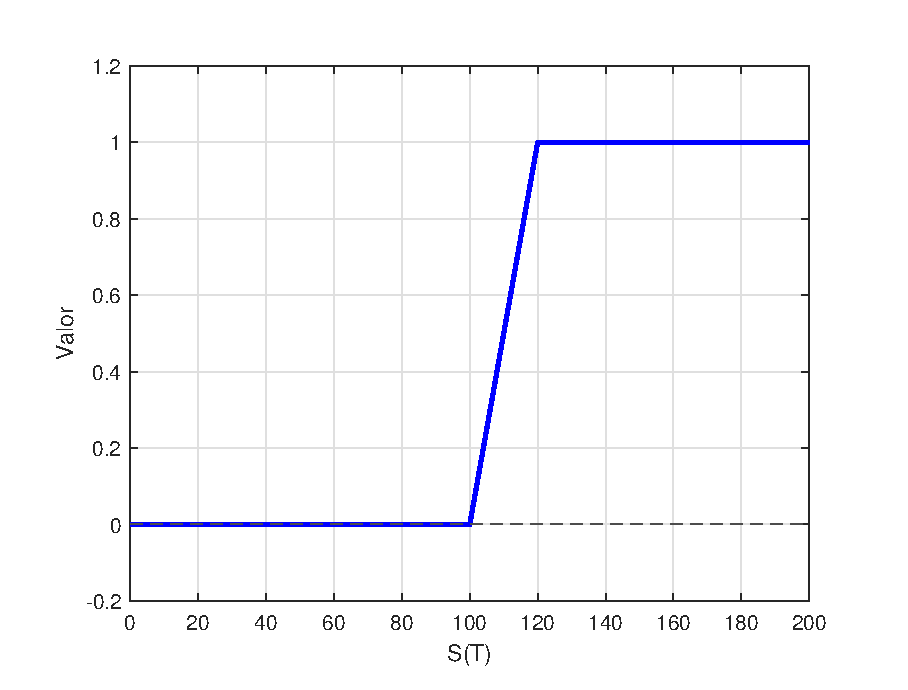
\includegraphics[width=0.5\linewidth]{Imagenes/Parte1/2_Derivados/BullPayoff.eps}
        \caption{Payoff de Bull Spread a vencimiento (normalizado)}
    \end{figure}
    Para normalizarlo se divide por $E_2-E_1$
    \item \textbf{Bear Spread (Spread Bajista)}: consiste consiste en comprar opción \textbf{put} con strike más alto $E_2$ y vender otra con strike más bajo $E_1$ ($E_1<E_2$). Hay beneficio si el subyacente \textbf{baja}, pero está limitado a diferencia $E_2-E_1$. Su payoff es:
     \[\boxed{\max(E_2-S, 0) - \max(E_1-S, 0)}\]
    \begin{figure}[H]
        \centering
        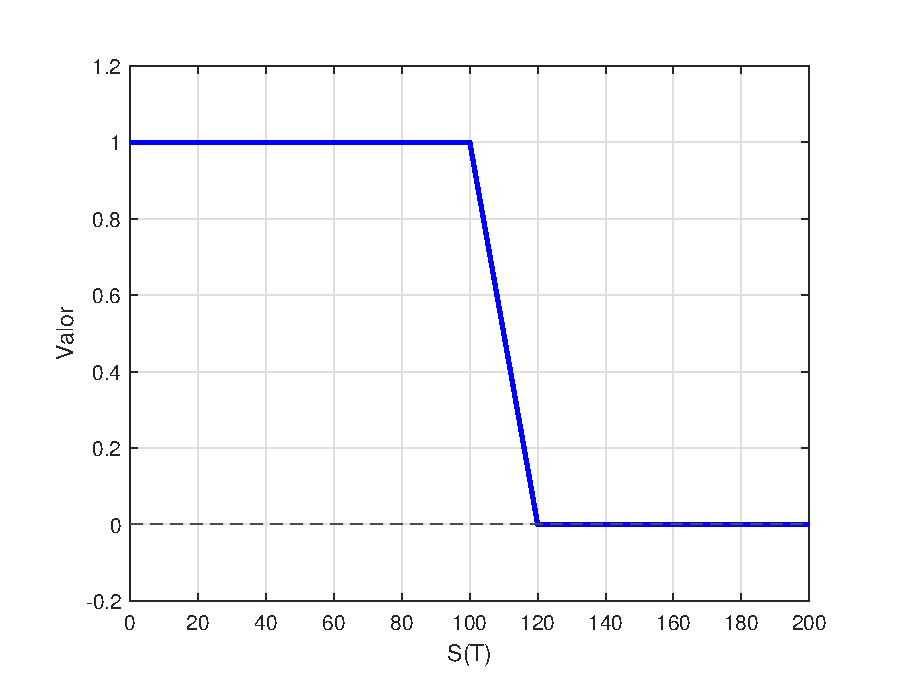
\includegraphics[width=0.5\linewidth]{Imagenes/Parte1/2_Derivados/BearPayoff.eps}
        \caption{Payoff de Bear Spread a vencimiento (normalizado)}
    \end{figure}
    Para normalizarlo se divide por $E_2-E_1$
    \item \textbf{Straddles}: comprar una call y una put con mismo strike y mismo expirity. Beneficio depende de la magnitud del movimiento del subyacente, pero costo alto por primas de dos opciones. Se suele hacer cuando hay un anuncio importante. Su payoff es:
    \[\boxed{\max(S-E, 0) + \max(E-S, 0)}\]
    \begin{figure}[H]
        \centering
        \includegraphics[width=0.5\linewidth]{Imagenes/Parte1/2_Derivados/StraddlePayoff.eps}
        \caption{Payoff de Straddle}
    \end{figure}
    \item \textbf{Strangle}: similar a straddles, pero con strikes distintos. Es más barato pero precisa de mayores cambios en el subyacente para que haya beneficios. Su payoff es:
    \[\boxed{\max(S-E_C, 0) + \max(E_P-S, 0)}\]
    Según los strikes pueden ser:
    \begin{itemize}
        \item \textbf{Out-of-the-Money Strangle (OTM)}: se compra call con strike por encima de precio actual y put con strike por debajo de actual. Es más barato (primas bajas) pero se necesita un movimiento grande del subyacente.
        \begin{figure}[H]
            \centering
            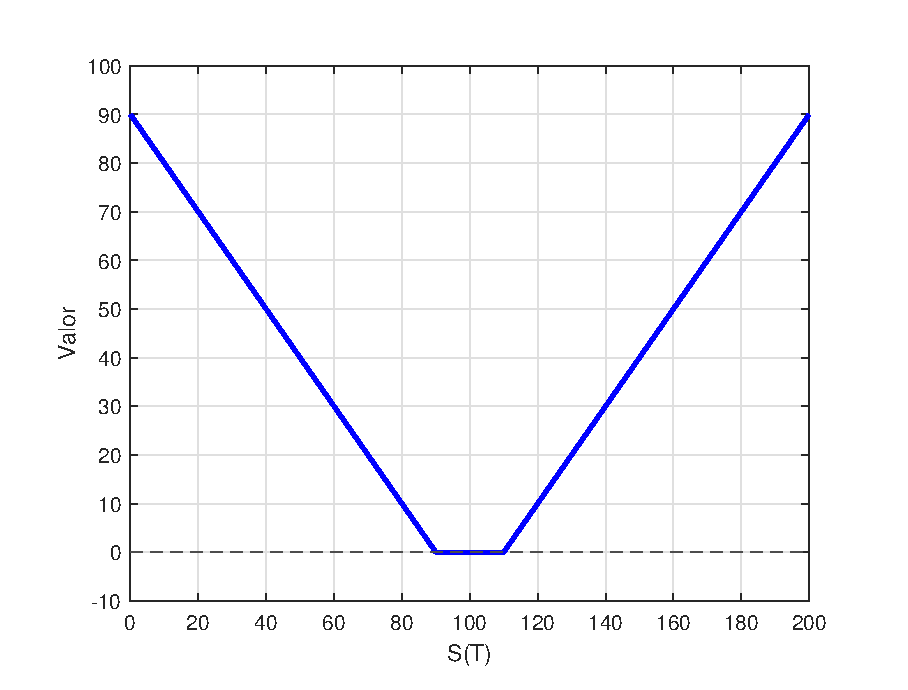
\includegraphics[width=0.5\linewidth]{Imagenes/Parte1/2_Derivados/StrangleOTMPayoff.eps}
            \caption{Payoff de Strangle OTM}
        \end{figure}
        \item \textbf{In-the-Money Strangle (ITM)}: se compra call con strike por debajo de precio actual y put con strike por encima de actual. Algo más caro (por primas) que OTM, pero un poco más seguro.
        \begin{figure}[H]
            \centering
            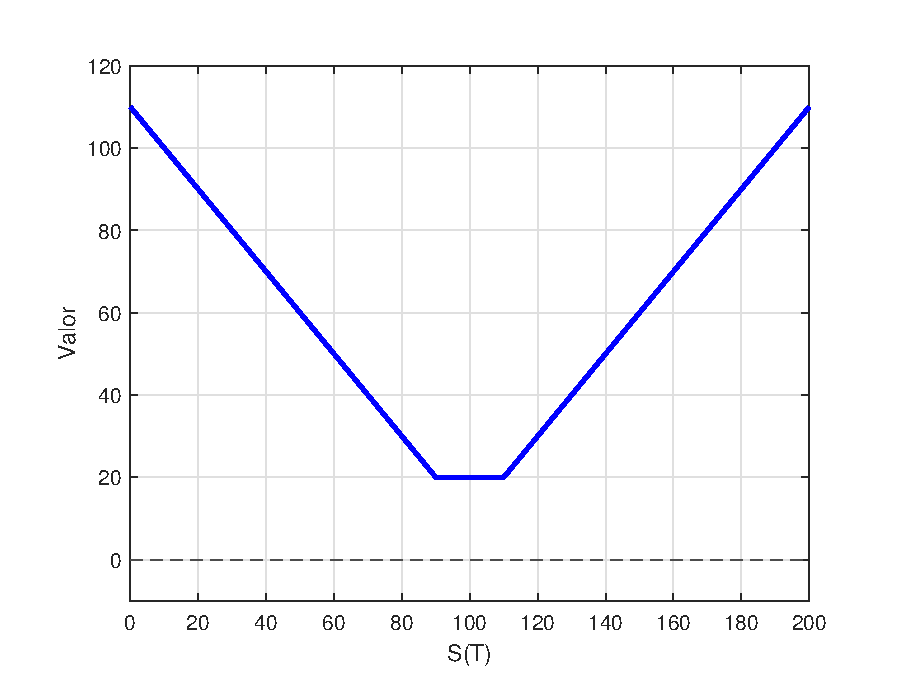
\includegraphics[width=0.5\linewidth]{Imagenes/Parte1/2_Derivados/StrangleITMPayoff.eps}
            \caption{Payoff de Strangle ITM}
        \end{figure}
    \end{itemize}
    \item \textbf{Risk Reversal}: comprar una call con strike mayor que el precio actual y vender una put con un strike inferior al precio actual. Se apuesta a que el subyacente va a subir (y que como mucho no va a bajar demasiado). Si el activo baja se pierde dinero, pero las primas son más baratas. Su payoff sería:
    \[\boxed{\max(S-E_C, 0) - \max(E_P-S, 0)}\]
    \begin{figure}[H]
        \centering
        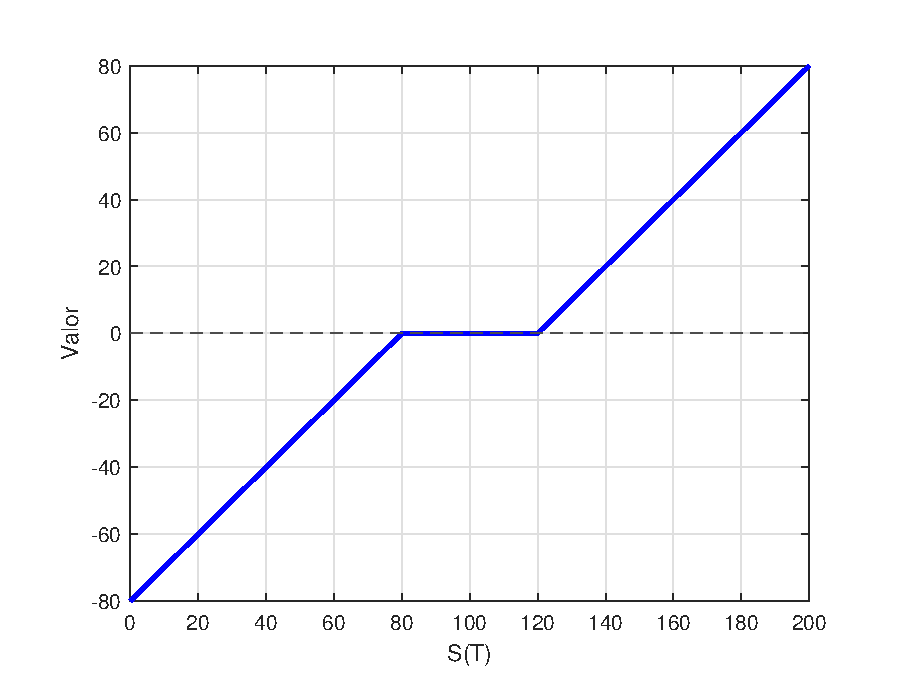
\includegraphics[width=0.5\linewidth]{Imagenes/Parte1/2_Derivados/RiskReversalPayoff.eps}
        \caption{Payoff de Risk Reversal a vencimiento}
    \end{figure}
    \item \textbf{Butterflies}: se compra una call ITM ($E_{C_{ITM}}$), se venden dos calls ATM (at-the-money) ($E_{C_{ATM}}$) y se compra una call OTM ($E_{C_{OTM}}$). Es decir, $E_{C_{ITM}}<E_{C_{ATM}}<E_{C_{OTM}}$. Además, generalmente se cumple que $E_{C_{OTM}} - E_{C_{ATM}} = E_{C_{ATM}} - E_{C_{ITM}}$. Se usa cuando se espera que el subyacente esté cerca de cierto precio central y haya poca volatilidad. Su payoff es:
    \[\boxed{\max(S-E_{C_{ITM}}, 0) - 2\max(S-E_{C_{ATM}}, 0) + \max(S-E_{C_{OTM}}, 0)}\]
    \begin{figure}[H]
        \centering
        \includegraphics[width=0.5\linewidth]{Imagenes/Parte1/2_Derivados/ButterflyPayoff.eps}
        \caption{Payoff de Butterfly a vencimiento}
    \end{figure}
    \item \textbf{Condors}: parecido a butterflies, se compra call con strike $E_1$, se vende call con strike $E_2$, se vende call con strike $E_3$, y se compra call con strike $E_4$ tal que $E_1<E_2<E_3<E_4$. Además, generalmente se cumple que $E_2-E_1=E_4-E_3$. Se obtienen ganancias máximas si el subyacente se mantiene entre $E_2$ y $E_3$. Su payoff es:
    \[\boxed{\max(S-E_1, 0) - \max(S-E_2, 0) - \max(S-E_3, 0) + \max(S-E_4, 0)}\]
    \begin{figure}[H]
        \centering
        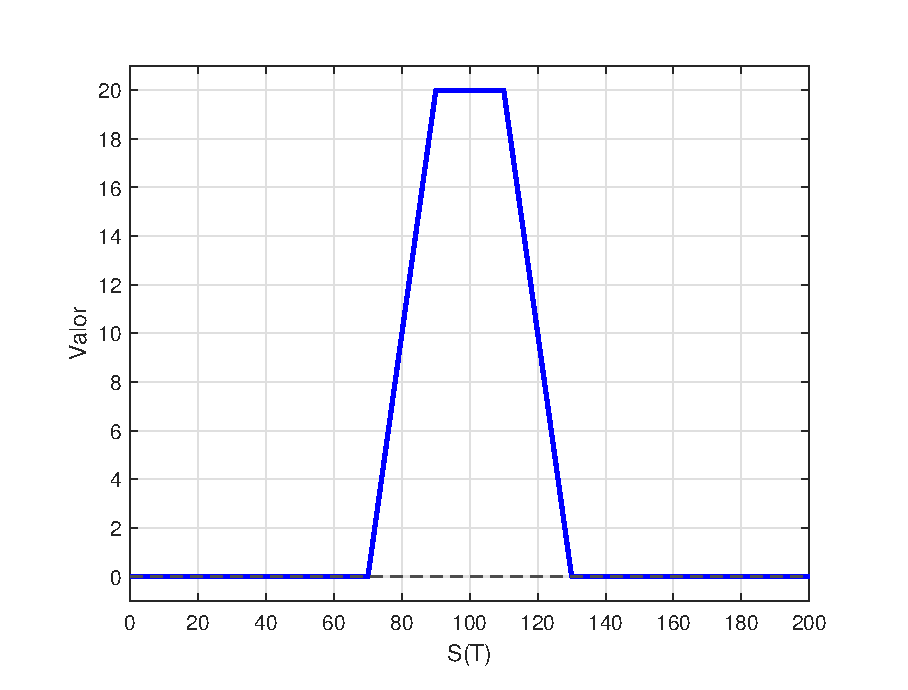
\includegraphics[width=0.5\linewidth]{Imagenes/Parte1/2_Derivados/CondorsPayoff.eps}
        \caption{Payoff de Condors a vencimiento}
    \end{figure}
\end{itemize}



\subsection{Opciones a largo plazo}
\begin{itemize}
    \item \textbf{LEAPS/ long-term equity anticipation securities}: opciones con hasta 3 años de fecha de vencimiento. Usualmente vencen en enero. Se suelen emitir a 3 precios de ejercicio: ATM (precio actual), 20\% ITM (más favorable para el comprador) o 20\% OTM (más especulativo).
    \item \textbf{FLEX/ FLexible EXchange-traded options}: permiten más personalización de la opcion de la fecha de vencimiento (hasta 5 años), el strike o el tipo de ejercicio (europeo o americano).
\end{itemize}


\subsection{Otros derivados}
\begin{itemize}
    \item \textbf{Warrants}: parecido a opciones call, pero emitido por la propia empresa del subyacente que da derecho a comprar acciones \textit{nuevas} (frente a acciones ya existentes en las opciones) emitidas por la empresa. Tiene plazos largos, de hasta 5 años.
    \item \textbf{Convertible bonds/ CBs}: bono normal que paga cupones y un capital a vencimiento, pero que tiene la opción de convertirse en acciones antes de vencimiento (perderías los cupones siguientes). Se comporta como una opción americana.
\end{itemize}











  \newpage
  \section{Productos de renta fija: bonos}



\subsection{Contratos simples de renta fija}

\subsubsection{Bonos de cupón cero}
Es un contrato que paga una contidad fija conocida (\textbf{principal}) en una fecha determinada (\textbf{maturity date}) $T$. Dicho valor se debe actualizar para calcular su precio.



\subsubsection{Bonos con cupón (coupon-bearing bond)}
Además de pagar el principal a fecha de vencimiento, paga \textbf{cupones} en ciertas fechas preestablecidas. Los cupones suelen ser un porcentaje del principal y se suelen pagar en periodos regulares.



\subsubsection{Money Market Account}
Cuentas de dinero (p.e.\ en el banco) que acumulan intereses compuestos de vez en cuando. El interés suele ser a corto plazo e impredecible, por lo que es ``arriesgado''. Tiene la ventaja de ser flexible (lo puedes mover cuando quieras).



\subsubsection{Floating Rate Bonds}
Los bonos de tasa flotante son bonos cuya tasa de interés está ligada a un índice de referencia  como el LIBOR (p.e.\ se puede recibir LIBOR+1\%). Protegen al inversor contra subidas de interés pero tiene poca flexibilidad (hay que esperar a vencimiento) y hay incertidumbre de lo que se va a recibir.



\subsubsection{Forward Rate Agreements (FRA)}
Se fija una tasa de interés fija sobre un principal. Una parte paga el principal en $T_1$ y la otra parte lo devuelve con los intereses acordados en $T_2 > T_1$. El valor del contrato al inicio suele no ser cero, por lo que puede haber un pago inicial entre las partes.



\subsubsection{Repos}
Es un acuerdo de recompra. Consiste en vender un activo financiero a otra parte y acordar recomprarlo en una fecha y cantidad fijada. El precio de recompra suele ser mayor que el de venta, y la diferencia implica un tipo de interés llamado \textbf{repo rate}. El más común es el \textit{overnight repo}, que se renegocia diariamente. Si el acuerdo dura más de 30 días se denomina \textit{term repo}. Un \textbf{reverse repo} es la operación inversa: la compra de un valor con el compromiso de venderlo posteriormente.



\subsubsection{Bonos separables (STRIPS)}
‘Separate Trading of Registered Interest and Principal of Securities’. Consisten en separar los cupones y el principal de los bonos tradicionales, creando así bonos artificiales de cupón cero con vencimientos más largos de los que normalmente estarían disponibles.

Por ejemplo se ha comprado un bono con cupones que dan 5\euro\ al año. Se pueden vender cada uno de esos cupones como bonos de cupón cero, y valdrían los 5\euro\ actualizados.



\subsubsection{Amortización}
El principal va disminuyendo poco a poco durante la vida del contrato y los intereses se calculan sobre el principal pendiente. 

La amortización puede ser fija (con un calendario conocido de antemano) o depender de algún índice (por ejemplo, si el índice sube, el principal se amortiza más rápido).

\subsubsection{Cláusula de rescate anticipado (Call Provision)}
Es una cláusula que se pone a contratos de renta fija que permite al emisor recomprar el contrato en ciertas fechas o periodos por un importe preestablecido. Esto reduce el valor del contrato para el inversor.






\subsection{Mercado internacional de bonos}
\begin{itemize}
    \item \textbf{USA}: 
    \begin{itemize}
        \item \textbf{Bill}: maturity menor que un año y normalmente sin cupón.
        \item \textbf{Note}: maturity entre 2 y 10 años, con cupón cada 6 meses.
        \item \textbf{Bond}: maturity mayor que 10 años, con cupón cada 6 meses.
        \item \textbf{Yankees}: comerciados en USA por instituciones extranjeras.
    \end{itemize}
    \item \textbf{UK}: los emitidos por el gobierno se llaman \textbf{gilts}. Incluyen bonos \textit{callable, irredeemable, convertible} o \textit{index-linked} ligados a Retail Price Index (RPI). Más adelante se explicará que es cada cosa.
    \item \textbf{Japón}: \textbf{Japanese Government Bonds (JGBs)} pueden ser a corto plazo (letras del tesoro, sin cupones), plazo medio (con o sin cupones), largo plazo (maturity de 10 años, cupones cada 6 meses) o plazo muy largo (maturity de 20 años, cupones cada 6 meses). Los emitidos en yenes por instituciones extranjeras son bonos \textbf{Samurai}.
\end{itemize}







\subsection{Rentabilidad de bonos (Yield)}
Existen varias maneras de calcular la rentabilidad de un bono:
\begin{itemize}
    \item \textbf{Current Yield}:
    \[
        \frac{\text{ingresos anuales por cupones}}{\text{precio bono}}
    \]
    Es útil solo para bonos a corto plazo. No tiene en cuenta el valor temporal del dinero ni el principal.
    \item \textbf{Yield to Maturity (YTM)/ Internal Rate of Return (IRR)/ tasa interna de rendimiento (TIR)}: tiene en cuenta el valor temporal del dinero y el principal. El YTM o IRR $y$ se calcula como:
    \[
        \boxed{ B = \frac{P}{(1+y)^T} + \sum_{t=1}^{T} \frac{C_t}{(1+y)^t} }
    \]
    en el caso discreto o como
    \[
        \boxed{ B = P e^{-yT} + \sum_{t=1}^{T} C_t e^{-yt}}
    \]
    en el caso continuo, donde $B$ es el precio del bono, $P$ es el valor nominal, $C$ es el cupón y $T$ es el tiempo hasta el vencimiento. Para obtener $y$ se usan métodos numéricos.
\end{itemize}




\subsection{Yield Curve}
Muestra cómo varía el rendimiento de los bonos en función de su vencimiento. Es útil para medir las expectativas de una economía:
\begin{itemize}
    \item \textbf{Normal Yield Curve}: los bonos a largo plazo tienen mayor rendimiento que los a corto plazo, lo que indica una economía en crecimiento.
    \item \textbf{Inverted Yield Curve}: los bonos a corto plazo tienen mayor rendimiento que los a largo plazo, lo que puede indicar una recesión económica.
    \item \textbf{Flat Yield Curve}: los rendimientos son similares para todos los plazos, lo que puede indicar incertidumbre económica.
\end{itemize}
\begin{figure}[H]
    \centering
    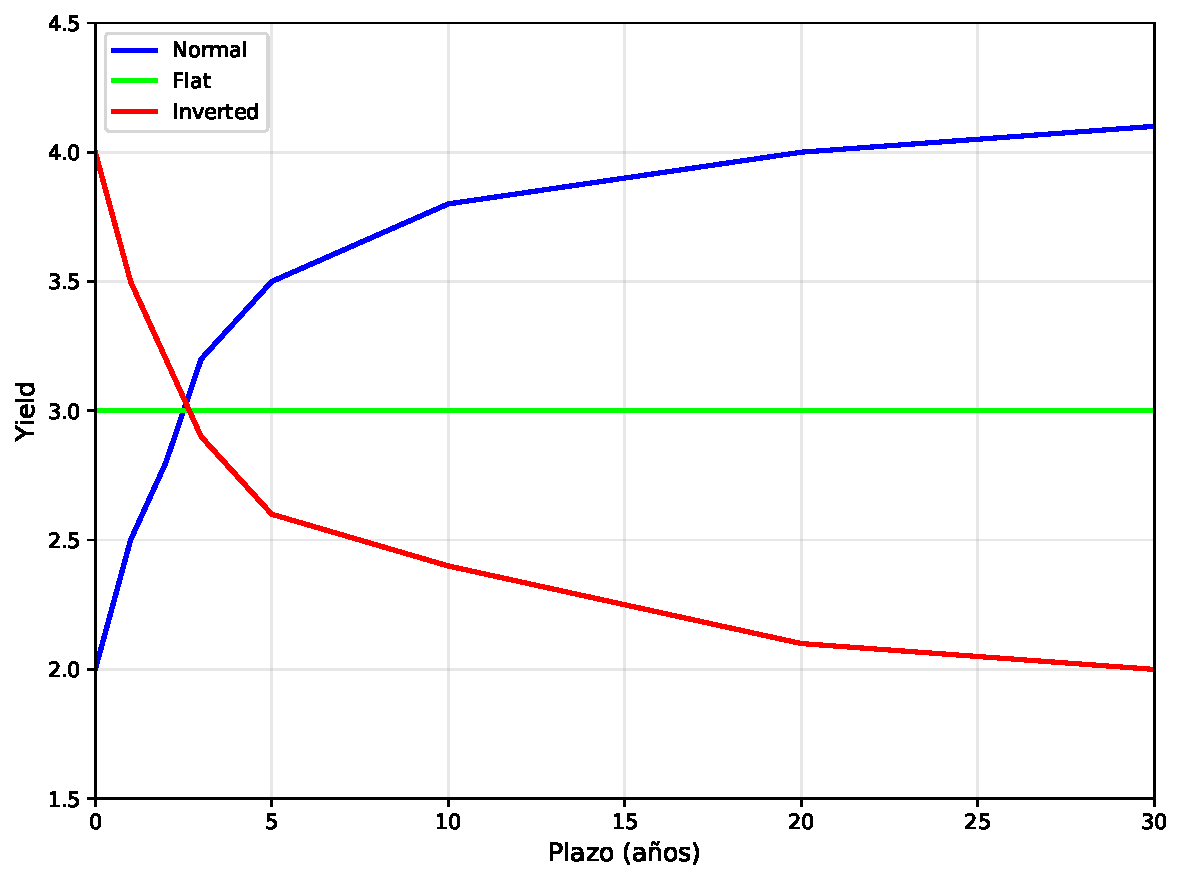
\includegraphics[width=0.65\linewidth]{Imagenes/Parte1/11_Prods_renta_fija/Yield_Curve.pdf}
    \caption{Yield Curve}
\end{figure}




\subsection{Duración}
Hay dos maneras de definir la duración de un bono:
\begin{itemize}
    \item \textbf{Duración modificada}: mide la sensibilidad del precio del bono ante pequeños cambios en la tasa de interés. P.e.\ si la duración es de 5.1, entonces un aumento  del 1\% del interés reduce el precio del bono un 5.1\%. Se calcula como:
    \[
        \boxed{D_{\text{mod}} =  -\frac{1}{B}\frac{\partial B}{\partial y}}
    \]
    \item \textbf{Duración Macaulay}: es el tiempo promedio ponderado hasta que se reciben los flujos del bono. P.e.\ si la duración es de 4.2, significa que, en promedio, el inversor recupera su dinero en 4.2 años. Se calcula como:
    \[
        \boxed{D_{\text{mac}} = (1+y)D_{\text{mod}} = -\frac{1+y}{B}\frac{\partial B}{\partial y}}
    \]
\end{itemize}

Las derivadas para el caso discreto y continuo son:
\begin{itemize}
    \item Caso discreto:
    \begin{align}\label{eq:derivadas_bono_discreto}
        B &= \frac{P}{(1+y)^T} + \sum_{t=1}^{T} \frac{C_t}{(1+y)^t} \notag \\
        \frac{\partial B}{\partial y} &= -\frac{P T}{(1+y)^{T+1}} - \sum_{t=1}^{T} \frac{C_t t}{(1+y)^{t+1}} = - \frac{1}{1+y}\left( \frac{P T}{(1+y)^{T}} + \sum_{t=1}^{T} \frac{C_t t}{(1+y)^{t}} \right) \\
        \frac{\partial^2 B}{\partial y^2} &= \frac{P T (T+1)}{(1+y)^{T+2}} + \sum_{t=1}^{T} \frac{C_t t (t+1)}{(1+y)^{t+2}} = \frac{1}{(1+y)^2}\left( \frac{P T (T+1)}{(1+y)^{T}} + \sum_{t=1}^{T} \frac{C_t t (t+1)}{(1+y)^{t}} \right)  \notag
    \end{align}
    \item Caso continuo:
    \begin{align}\label{eq:derivadas_bono_continuo}
        B &= P e^{-yT} + \sum_{t=1}^{T} C_t e^{-yt}  \notag \\
        \frac{\partial B}{\partial y} &= -P T e^{-yT} - \sum_{t=1}^{T} C_t t e^{-yt} \\
        \frac{\partial^2 B}{\partial y^2} &= P T^2 e^{-yT} + \sum_{t=1}^{T} C_t t^2 e^{-yt}  \notag
    \end{align}
\end{itemize}
por lo que las duraciones son:
\begin{itemize}
    \item Caso discreto:
    \begin{align*}
        D_{\text{mod}} &=  -\frac{1}{B}\frac{\partial B}{\partial y} = -\frac{1}{B}\left(- \frac{1}{1+y}\left( \frac{P T}{(1+y)^{T}} + \sum_{t=1}^{T} \frac{C_t t}{(1+y)^{t}} \right)\right) \\
        &= \boxed{ \frac{1}{1+y}\left( \frac{ \frac{P T}{(1+y)^{T}} + \sum_{t=1}^{T} \frac{C_t t}{(1+y)^{t}} }{ \frac{P}{(1+y)^T} +\sum_{t=1}^{T} \frac{C_t}{(1+y)^t} } \right) } \\
        D_{\text{mac}} &= \boxed{ (1+y)D_{\text{mod}} = \frac{ \frac{P T}{(1+y)^{T}} + \sum_{t=1}^{T} \frac{C_t t}{(1+y)^{t}} }{ \frac{P}{(1+y)^T} +\sum_{t=1}^{T} \frac{C_t}{(1+y)^t} } }
    \end{align*}
    \item Caso continuo:
    \begin{align*}
        D_{\text{mod}} &=  -\frac{1}{B}\frac{\partial B}{\partial y} = \boxed{ \frac{ P T e^{-yT} + \sum_{t=1}^{T} C_t t e^{-yt} }{ P e^{-yT} + \sum_{t=1}^{T} C_t e^{-yt} } } \\
        D_{\text{mac}} &= (1+y)D_{\text{mod}} = \boxed{ (1+y)\frac{ P T e^{-yT} + \sum_{t=1}^{T} C_t t e^{-yt} }{ P e^{-yT} + \sum_{t=1}^{T} C_t e^{-yt} } }
    \end{align*}
\end{itemize}




\subsection{Convexividad}
Es otro orden para medir la sensibilidad del precio del bono frente a cambios del interés. Una mayor convexidad implica menor pérdida ante subidas de tasas y mayor ganancia ante bajadas. Se calcula como:
\[
    \boxed{C = \frac{1}{B}\frac{\partial^2 B}{\partial y^2}}
\]
observando las derivadas calculadas en~\eqref{eq:derivadas_bono_discreto} y~\eqref{eq:derivadas_bono_continuo}tiene que:
\begin{itemize}
    \item Caso discreto:
    \[
        C = \frac{1}{B}\frac{\partial^2 B}{\partial y^2} = \boxed{ \frac{1}{(1+y)^2} \frac{ \frac{P T (T+1)}{(1+y)^{T}} + \sum_{t=1}^{T} \frac{C_t t (t+1)}{(1+y)^{t}} }{ \frac{P}{(1+y)^T} + \sum_{t=1}^{T} \frac{C_t}{(1+y)^t}}  }
    \]
    \item Caso continuo:
    \[
        C = \frac{1}{B}\frac{\partial^2 B}{\partial y^2} = \boxed{ \frac{P T^2 e^{-yT} + \sum_{t=1}^{T} C_t t^2 e^{-yt}}{P e^{-yT} + \sum_{t=1}^{T} C_t e^{-yt}} }
    \]
\end{itemize}






\subsection{Intereses dependientes del tiempo (Time-Dependent Interest Rates)}
Se considera un interés dependiente del tiempo $r(t)$, por lo que el valor del bono también es dependiente del tiempo $B(t)$. Se considera que el principal 1, por lo que $B(T)=1$. Todas las constantes que se calculan a continuación son relativas a esta condición.

Se tiene por una parte que la variación del valor del bono es:
\[
    \frac{dB}{dt} = \frac{dB}{dt} \Rightarrow dB = \frac{dB}{dt} dt
\]
este argumento se puede justificar de forma más estricta con intervalos infinitesimales o aproximaciones de Taylor. Para evitar arbitraje se iguala al interés:
\begin{align}\label{eq:interes_dependiente_tiempo}
    dB = \frac{dB}{dt} dt = r(t) B dt \Rightarrow B(t; T) = e^{\int_{t}^{T} r(\tau) d\tau}
\end{align}

Estudiando ahora el caso de un bono con cupones, se tiene que se ha recibido un cupón $K(t)dt$ en el periodo $[t, t+dt]$, por lo que la variación del valor del bono es:
\[
    dB = \left( \frac{dB}{dt} + K(t) \right) dt
\]
que igualando al interés:
\[
    \frac{dB}{dt} + K(t) = r(t) B \Rightarrow \boxed{B(t; T) = e^{\int_{t}^{T} r(\tau) d\tau} \left( 1 + \int_t^T K(t') e^{\int_{t}^{T} r(\tau) d\tau} dt' \right)}
\] 
habiendo elegido las constantes para que $B(T)=1$.







\subsection{Tasas Forward y bootstrapping}\label{sec:forward_bootstrapping}
Es la tasa de interés esperada de un bono sabiendo la tasa de interés actual de varios bonos de cupón cero con diferentes vencimientos. 

En el caso continuo, y que todo es diferenciable correctamente, no hace falta más que la ecuacion~\eqref{eq:interes_dependiente_tiempo} para calcular la tasa forward $f(t, T)$ entre dos fechas $t$ y $T$. 
\[
    Z(t; T) = e^{\int_{t}^{T} r(\tau) d\tau} \Rightarrow r(T) = -\frac{\partial}{\partial T} \left( \ln(Z(t;T)) \right) \Rightarrow F(t;T) = -\frac{\partial}{\partial T} \left( \ln(Z(t;T)) \right) 
\]
que en términos de rendimiento se tiene que
\[
    Z(t; T) = e^{-y(t;T)(T-t)} \Rightarrow \boxed{F(t;T) = y(t;T) + \frac{\partial y}{\partial T}}
\]



Para el caso discreto se consideran varios bonos de cupón cero ordenados según su vencimiento, siendo el primero el que tenga el vencimiento más temprano. Luego se tiene $Z_i^M$ siendo $i$ la posición en el ranking. EL primer bono tendrá tiene un interés implícito de
\[
    Z_1^M = e^{y_1(T_1-t)} \Rightarrow y_1 = \frac{\ln(Z_1^M)}{T_1-t}
\]
este es el interés que se usa para descontar desde el momento actual hasta  $T_1$ para todos los bonos e instrumentos. Por lo tanto el interés implícito del segundo bono sería
\[
    Z_2^M = e^{-y_1(T_1-t)} e^{y_2(T_2-T_1)} \Rightarrow y_2 = \frac{\ln(Z_2^M/Z_1^M)}{T_2-T_1}
\]
se puede seguir este proceso de forma iterativa para los bonos que hagan falta. A esto se le llama \textbf{bootstrapping}.








  \newpage
  \section{Swaps}\label{sec:swaps}


Los \textbf{swaps} son contratos en los que dos partes acuerdan intercambiar flujos de efectivo futuro según una fórmula preestablecida. En un primer momento lo típico eran swaps de divisas, pero derivó en swaps de intereses.



\subsection{Swaps de intereses vainillas}
Contratos bastante comunes en los que se intercambian flujos de intereses. Por ejemplo, una parte paga un tipo fijo y la otra un tipo variable como el Euribor a 3 meses, 6 meses, etc. A vencimiento, los principales no se intercambian, solo los intereses.
\begin{figure}[H]
    \centering
    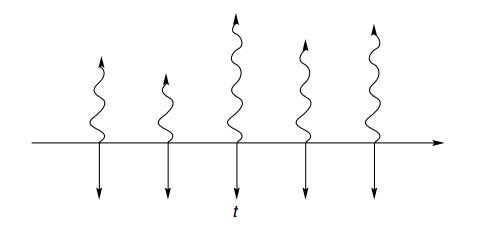
\includegraphics[width=0.65\linewidth]{Imagenes/Parte1/12_swaps/Interest_swap.png}
    \caption{Swaps de intereses vainillas}
\end{figure}
\subsubsection{Ejemplo de uso}
Dos empresas, A y B quieren pedir un préstamo, A quiere que sea variable y B que sea fijo. Los intereses que les cobran estan en la siguiente tabla:
\begin{table}[H]
    \centering
    \begin{tabular}[H]{|l|c|c|}
        \hline
        & \textbf{Fijo} & \textbf{Variable} \\
        \hline
        \textbf{A} & 7\% & \text{LIBOR a 6 meses} + 0.3\% \\
        \hline
        \textbf{B} & 8.2\% & \text{LIBOR a 6 meses} + 1\% \\
        \hline
    \end{tabular}
\end{table}
Luego si ambos piden el préstamos los intereses que pagan son:
\begin{itemize}
    \item A variable y B fijo:
    \[
        \text{LIBOR} + 0.3\% + 8.2\% = \text{LIBOR} + 8.5\%
    \]
    \item A fijo y B variable:
    \[
        7\% + \text{LIBOR} + 1\% = \text{LIBOR} + 8\%
    \]
\end{itemize}
Luego es mejor la segunda opción, pero como no es el tipo de interés que quieren cada uno, hacen un swap. Se reparten los inetreses extra de manera equitativa. Para dar la vuelta al tipo de interés, en el swap A le paga a B el LIBOR y B le paga una cantidad fija $x$\%. Entonces:
\begin{align*}
    \text{A: } & \underbrace{7\%}_{\text{int A fijo}} + \underbrace{\text{LIBOR}}_{\text{pago swap}} - \underbrace{x\% }_{\text{cobro swap}} + \underbrace{\frac{0.5}{2}\%}_{\text{int extra}} =  \underbrace{\text{LIBOR} + 0.3\%}_{\text{int A variable}} \Rightarrow x = 6.95\%\\
    \text{B: } & \underbrace{\text{LIBOR} + 1\%}_{\text{int B variable}} + \underbrace{x\%}_{\text{pago swap}} - \underbrace{\text{LIBOR}}_{\text{cobro swap}} + \underbrace{\frac{0.5}{2}\%}_{\text{int extra}} =  \underbrace{8.2\%}_{\text{int B fijo}} \Rightarrow x = 6.95\%
\end{align*}
por lo tanto, las empresas A y B pagan un interés:
\begin{align*}
    \text{A: } & \underbrace{7\%}_{\text{int A fijo}} + \underbrace{\text{LIBOR}}_{\text{pago swap}} - \underbrace{6.95\% }_{\text{cobro swap}} =  \text{LIBOR} + 0.05\% \\
    \text{B: } & \underbrace{\text{LIBOR} + 1\%}_{\text{int B variable}} + \underbrace{6.95\%}_{\text{pago swap}} - \underbrace{\text{LIBOR}}_{\text{cobro swap}} =  7.95\%
\end{align*}
que es tipo de interés que quería cada empresa y es mejor que si hubieran pedido el préstamo directamente con los intereses de la tabla.









\subsection{Relación entre swaps y bonos: obtener valor justo del interés fijo}
En primer lugar, el interés fijo se puede ver como un bono de cupón cero. Por lo tanto, el total de pagos por parte del interés fijo es
\[
    r_s\tau \sum_{i=1}^N Z(t;T_i)
\]
donde $r_s$ es el interés (p.e.\ anual), $\tau$ es el tiempo entre pagos (escrito en la misma escala que el interés, p.e.\ 0.5 años) y $Z(t;T)$ es el valor actualizado de un bono de cupón cero y principal 1.

Por otro lado, se debe escribir el valor de los intereses variables pagados en términos de un bono. Se tiene el siguiente esquema para el pago del interés variable en tiempo $T_i$:
 \begin{figure}[H]
    \centering
    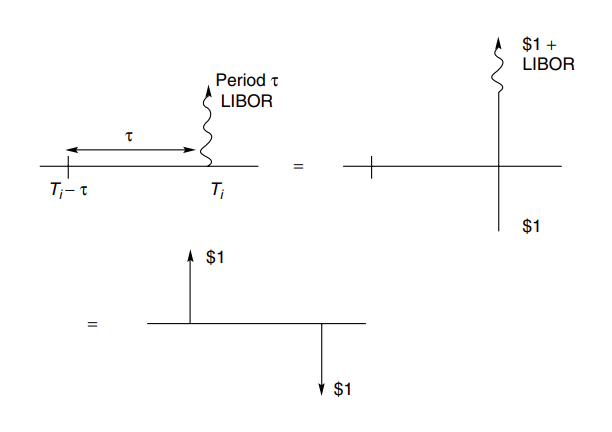
\includegraphics[width=0.65\linewidth]{Imagenes/Parte1/12_swaps/Relacion_Swaps_Bonos.png}
    \caption{Interes variable swap}
\end{figure}
En la primera imagen se representa el interés variable $r_\tau \tau$ en tiempo $T_i$, mientras que en la segunda se suma y resta un dolar en tiempo $T_i$. Por definidición, un dolar más el interés variable $r_\tau \tau$ en tiempo $T_i$ es igual que ese mismo dolar en tiempo $T_{i-\tau}$, lo que da lugar a la tercera imagen. Esta tercera imagen implica que el pago de un interés variable en tiempo $T_i$ es igual que pagar un bono de cupón cero con principal 1 en tiempo $T_i$ y venderlo en tiempo $T_{i-\tau}$.

Si se sigue este esquema para todos los pagos de interés variable, se van cancelando los depósitos y retiros quedando solo el primero y el ultimo.
Por otro lado, se debe escribir el valor de los intereses variables pagados en términos de un bono. Se tiene el siguiente esquema para el pago del interés variable en tiempo $T_i$:
 \begin{figure}[H]
    \centering
    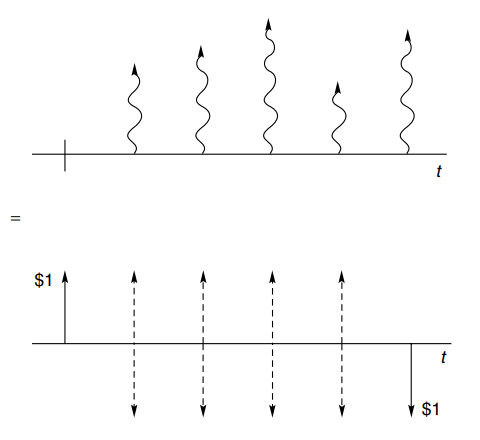
\includegraphics[width=0.65\linewidth]{Imagenes/Parte1/12_swaps/Interes_variable_swaps.png}
    \caption{Todos los intereses variables swap}
\end{figure}
Por lo tanto, el total de pagos por parte del interés variable es
\[
    1 - Z(t;T_N)
\]
siendo $Z(t;T_N)$ el valor actualizado de un bono de cupón cero y principal 1 (que es lo mismo que actualizar 1\$). 

Luego sumando el total de pagos de la parte del inetrés fijo y restando la parte del interés variable, el contrato swap para la parte variable es de:
\[
    r_s\tau \sum_{i=1}^N Z(t;T_i) - (1 - Z(t;T_N)) = \boxed{r_s\tau \sum_{i=1}^N Z(t;T_i) - 1 + Z(t;T_N)}
\]
para que el contrato tenga valor cero, el interés fijo debe ser debe
\begin{align}\label{eq:int_var}
    r_s\tau \sum_{i=1}^N Z(t;T_i) - 1 + Z(t;T_N) = 0 \Rightarrow \boxed{r_s = \frac{1 - Z(t;T_N)}{\tau \sum_{i=1}^N Z(t;T_i)}}
\end{align}
En vez de cero también se le puede dar cualquier valor.




\subsection{Bootstrapping}
El resultado anterior se puede usar para hacer el bootstrapping descrito en la sección~\ref{sec:forward_bootstrapping} para conseguir el valor de cupones cupón cero. Usando la ecuación~\eqref{eq:int_var}, se obtiene el valor de un bono de cupón cero y vencimiento $T_i$
\[
    r_s(T_1) = \frac{1 - Z(t;T_1)}{\tau Z(t;T_1)} \Rightarrow \boxed{Z(t;T_1) = \frac{1}{1+r_s(T_1)\tau}}
\]
y luego de forma iterativa
\[
    \boxed{Z(t; T_{j+1}) = \frac{1 - r_s(T_{j+1})\tau \sum_{i=1}^{j} Z(t; T_i)}{1 + r_s(T_{j+1})\tau}}
\]







\subsection{Otras características de contratos swap}
\begin{itemize}
    \item \textbf{Swaps Callable y puttable}: Permiten a un lado cerrar el contrato antes de vencimiento. Matemáticamente son del tipo opciones americanas, que se verán más adelante. 
    \item \textbf{Extendible swaps}: se puede ampliar el vencimiento con la tasa swap original.
    \item \textbf{Index amortizing rate swaps}: mientras que en los swaps vainilla el principal es constante (aunque nunca se llegue a pagar), en estos swaps el principal cambia con el tiempo siguiendo un calendario y muchas veces ligado a algún índice.
\end{itemize}





\subsection{Otros tipos de swaps}
\begin{itemize}
    \item \textbf{Basis Rate Swap}: los intereses son ambos variables ligados a distintos índices. P.e.\ un banco saca swaps de LIBOR contra los intereses que dan en los préstamos (que normalmente van ligados) para reducir riesgos en caso que dejen estar correlacionados.
    \item \textbf{Equity Swaps}: una parte paga interés fijo o flotante y la otra paga el retorno total de un índice bursátil (como el S\&P 500, EuroStoxx, etc.) incluyendo dividendos.
    \item \textbf{Equity basis swap}: como el anterior pero con dos índices distintos.
    \item \textbf{Currency Swaps}: dos partes intercambian flujos de efectivo en distintas divisas. P.e.\ una parte paga 1000\$ y la otra 1000\euro\ a un tipo de cambio preestablecido. Normalmente se intercambia el principal al inicio y al final del contrato.
\end{itemize}









  \clearpage%
  \chapter{Aletoriedad}
  
\section{Algunas propiedades}

\subsection{Desigualdad de Jensen}
Sea la función convexa $f(S)$ (que se curva hacia arriba, con forma de cuenco) de la variable aleatoria $S$, entonces
\[\mathbb{E}[f(S)] \geq f(\mathbb{E}[S])\]
De hecho, la diferencia es de
\[\frac{1}{2}f''(\mathbb{E}[S])\mathbb{E}[\epsilon]\]
donde $\epsilon$ es la desviación de $S$ de la media, i.e $S=\mathbb{E}[S]+\epsilon$.


\subsection{Propiedad de Markov}
\textit{El futuro depende solo del presente, no del pasado.} Se usa en los caminos aleatorios para decir que el valor $S_t+1$ solo depende de $S_t$, es decir,
\[\mathbb{P}(X_{t+s} \in A \mid X_t = x, X_{t_1} = x_1, \ldots, X_{t_n} = x_n) 
= \mathbb{P}(X_{t+s} \in A \mid X_t = x)\]



\subsection{Propiedad de martingala}
\textit{Lo que esperas tener en el futuro, sabiendo todo hasta ahora, es exactamente lo que tienes ahora}. Es decir, el valor esperado de algo en un juego justo es exactamente lo que tienes ahora:
\[\mathbb{E}[S_i|S_j, j<i]=S_j\]



\subsection{Lema de Itô}
Sea
\[dS = a(S,t)dt + b(S,t)d\mathnormal{X}\]
entonces
\begin{equation}
    \boxed{dV = \left( \frac{dV}{dt} +  a\frac{dV}{dS} + \frac{1}{2}b^2\frac{d^2V}{dS^2} \right)dt + b\frac{dV}{dS}d\mathnormal{X}}
\end{equation}\label{Ito}
En el apéndice~\ref{CalcIto} se encuentra la fórmula para dimensiones mayores.

\subsection{Algunos ejemplos de caminos aleatorios}

\begin{itemize}
    \item \textbf{Brownian Motion with Drift}: $\boxed{dS = \mu dt + \sigma d\mathnormal{X}}$
    \begin{figure}[H]
        \centering
        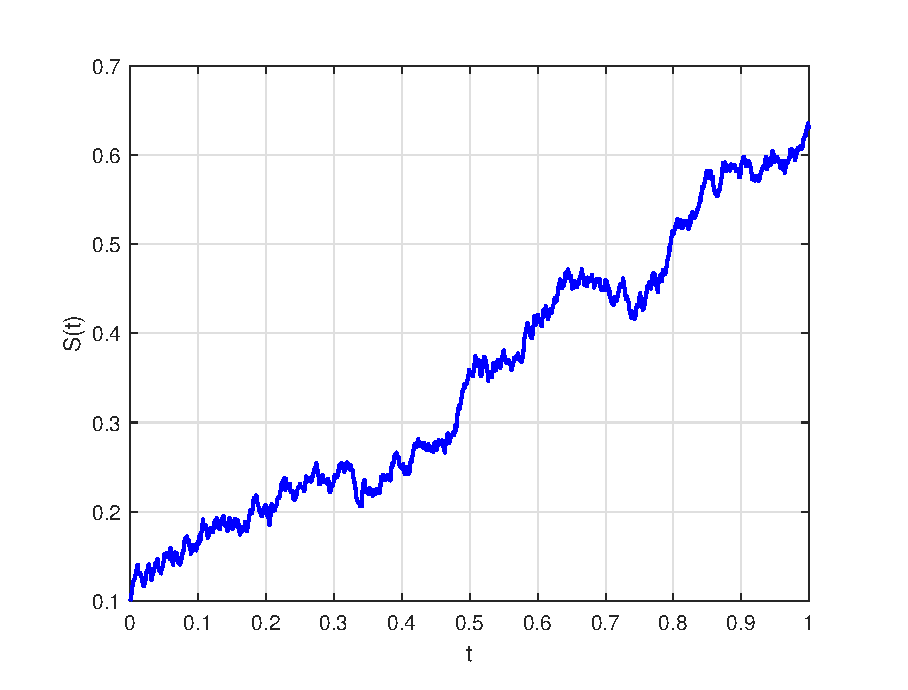
\includegraphics[width=0.65\linewidth]{Imagenes/Parte1/3_Aleatoriedad/BrownianMotionDrift.eps}
        \caption{Brownian Motion with Drift}
    \end{figure}
    \item \textbf{The Lognormal Random Walk}: $\boxed{dS = S\mu dt + S\sigma d\mathnormal{X}}$
    \begin{figure}[H]
        \centering
        \includegraphics[width=0.65\linewidth]{Imagenes/Parte1/3_Aleatoriedad/LognormalRandomWalk.eps}
        \caption{The Lognormal Random Walk}
    \end{figure}
    \item \textbf{A Mean-reverting Random Walk}: reversion a la media, cuando se esta fuera del crecimiento normal el camino tiende a corregirse.\\
    Su EDE es 
    \[
        \boxed{dS = \kappa(\theta+S) dt + \sigma d\mathnormal{X}}
    \]
    donde $\kappa$ es la velocidad de reversión a la media, $\theta$ es la tasa de interés a largo plazo y $\sigma$ es la volatilidad. Un ejemplo común es el modelo Vasicek para el ratio de interés, $dr = \kappa(\theta+r) dt + \sigma d\mathnormal{X}$
    \begin{figure}[H]
        \centering
        \includegraphics[width=0.65\linewidth]{Imagenes/Parte1/3_Aleatoriedad/MeanRevertingWalk.eps}
        \caption{Mean-reverting Random Walk}
    \end{figure}
\end{itemize}



\section{Función de densidad de transición}
Es la \textit{`probabilidad de que una variable aleatoria $y$ esté entre $a$ y $b$ en el instante futuro $t'$, sabiendo que ha empezado con un valor $y$ en el instante $t$`}. En concreto la función de densidad de transición $p(y, t; y', t')$ es:
\[
    \boxed{\text{Prob}(a<y'<b\text{ en }t' | y\text{ en }t) = \int_a^b p(y, t; y', t') dy'}
\]

\subsection{Ecuación de Fokker-Planck o de Kolmogorov hacia delante}
Se centra en cómo evoluciona la transición con respecto al tiempo futuro $t'$. Se enfoca en el destino del proceso y cómo cambia la probabilidad de estar en distintos valores futuros $y'$ a medida que avanza el tiempo $t'$. Sabiendo que la variable aleatoria cumple la EDE
\[
    dy = A(y, t) dt + B(y, t) d\mathnormal{X}
\]
entonces la función de densidad de transición es la solución de la ecuación diferencial parcial
\[
    \boxed{\frac{\partial p}{\partial t'} = \frac{1}{2} \frac{\partial^2}{\partial y'^2} \left( B(y', t')^2 p \right) - \frac{\partial}{\partial y'} \left( A(y', t') p \right)}
\]
por ejemplo para la EDE
\[
    dS = \mu S dt + \sigma S d\mathnormal{X}
\]
se tiene que reolver la EDP
\[
    \frac{\partial p}{\partial t'} = \frac{1}{2} \frac{\partial^2}{\partial S'^2} \left( \sigma^2 S'^2 p \right) - \frac{\partial}{\partial S'} \left( \mu S' p \right)
\]
que da como solución
\[
    p(S, t; S', t') = \frac{1}{\sigma S' \sqrt{2\pi (t'-t)}} \exp\left( -\frac{ \left( \log(S/S') + (\mu - \frac{1}{2}\sigma^2)(t'-t) \right)^2 }{ 2\sigma^2 (t'-t) } \right)
\]
\begin{figure}[H]
    \centering
    \begin{subfigure}[b]{0.45\linewidth}
        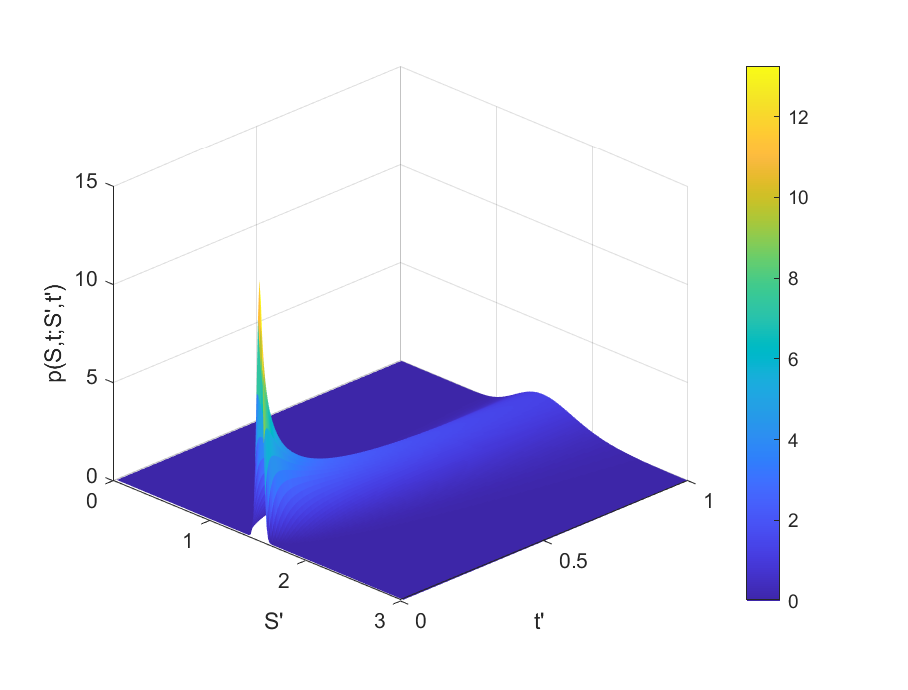
\includegraphics[width=\linewidth]{Imagenes/Parte1/3_Aleatoriedad/PDF_3D.eps}
    \end{subfigure}
        \begin{subfigure}[b]{0.45\linewidth}
        \includegraphics[width=\linewidth]{Imagenes/Parte1/3_Aleatoriedad/PDF_2D.eps}
    \end{subfigure}
    \caption{Función de densidad de transición}
\end{figure}



\subsubsection{Ecuación de Kolmogorov hacia detrás}
Se centra en cómo evoluciona la densidad de transición con respecto al tiempo actual $t$. Se enfoca más en el origen  y cómo cambian las probabilidades de llegar al punto $y'$, $t'$ dependiendo de donde se está en el momento. La EDP es
\[
    \boxed{\frac{\partial p}{\partial t} + \frac{1}{2} B(y, t)^2 \frac{\partial^2 p}{\partial y^2} + A(y, t) \frac{\partial p}{\partial y} = 0}
\]


\subsubsection{Distribución en estado estacionario (steady-state distribution)}
Son aquellas cuya función de densidad de transición $p(y, t; y', t')$ tiende, cuando $t' \to \infty$, a una distribución que ya no depende del estado inicial $y$ ni del tiempo $t$. Para eso se debe cumplir que el proceso sea homogéneo en el tiempo, i.e. $A$ y $B$ sean independientes de $t$ en el límite asintótico. Cuando se cumple la función de densidad de transición converge a $p_\infty(y')$ que satisface:
\[
    \boxed{\frac{1}{2} \frac{d^2}{dy'^2} \left( B_\infty^2 p_\infty \right) - \frac{d}{dy'} \left( A_\infty p_\infty \right) = 0}
\]
donde $A_\infty$ y $B_\infty$ son los valores de los coeficientes en el límite $t \to \infty$.








\section{Tiempos de primer escape (First-exit times)}\label{sec:FirstExitTimes}
El \textit{first-exit time} es el tiempo en el cual un camino aleatorio alcanza un cierto límite por primera vez. El objetivo de esta sección es calcular la probabilidad de que un camino aleatorio alcance cierto límite antes de cierto tiempo.
\begin{figure}[H]
    \centering
    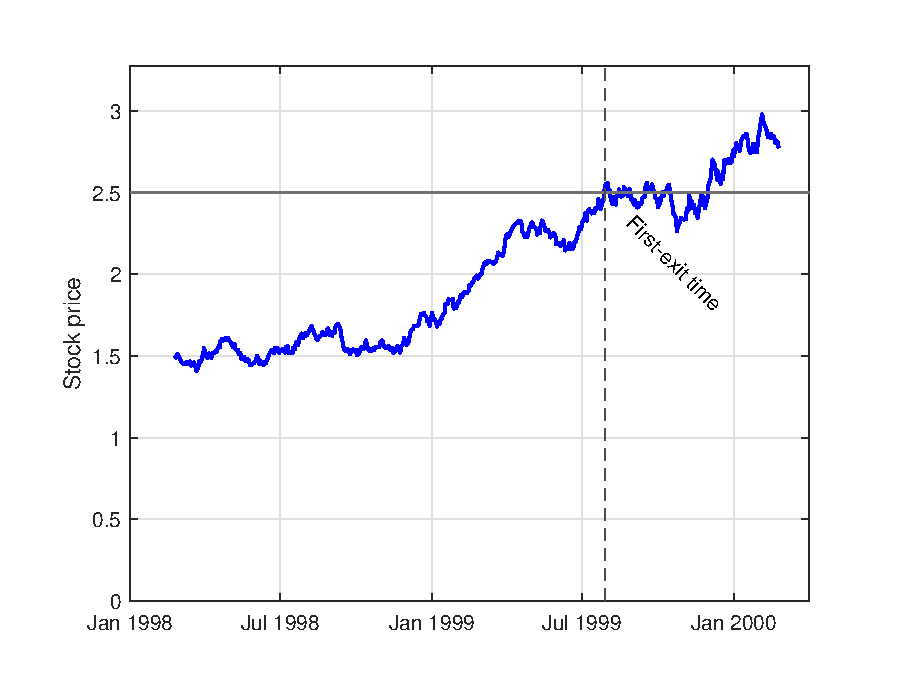
\includegraphics[width=0.65\linewidth]{Imagenes/Parte1/3_Aleatoriedad/First-exit_Time.eps}
    \caption{First-exit Time}
\end{figure}




\subsection{Funciones de distribución acumulada para first-exit times}
Se definde la función $C(y, t; t')$ como la probabilidad de que la variable $y$ salga de la región $\Omega$ antes del tiempo $t'$, habiendo empezado en $y$ en el tiempo $t$. Esta función puede interpretarse como una función de distribución acumulada para first-exit time. 

El objetivo es calcular la probabilidad de que un camino aleatorio abandone una región $\Omega$ antes de un tiempo dado $t'$. Para ello, se tiene que satisfacer el problema de la EDP hacia atrás:
\begin{equation}\label{eq:CumulatFirstExitTime}
    \boxed{
    \left\{
    \begin{array}{rlrl}
        \displaystyle\frac{\partial C}{\partial t} + \frac{1}{2} B(y, t)^2 \frac{\partial^2 C}{\partial y^2} + A(y, t) \frac{\partial C}{\partial y} = 0 &\quad& (y,t) \in \Omega\times(0, t') \\[2ex]
        C(y, t; t') = 1 && (y,t) \in \partial\Omega\times(0, t') \\[2ex]
        C(y, t'; t') = 0 && y \in \Omega \\
    \end{array}
    \right\}
    }
\end{equation}




\subsection{Tiempos de primer escape esperados (Expected first-exit times)}\label{sec:ExpectedFirstExitTimes}
Una vez calculado~\eqref{eq:CumulatFirstExitTime} es posile calcular el tiempo esperado de primer escape:
\[
    u(y, t) = \int_t^\infty (t' - t) \frac{\partial C}{\partial t'} dt' \overset{\text{partes}}{=} \int_t^\infty 1 - C(y, t; t') dt'
\]
por lo tanto,
\begin{align*}
    \frac{\partial u}{\partial t}  &= \frac{\partial}{\partial t} \left(\int_t^\infty 1 - C(y, t; t') dt' \right) \overset{\text{Leibniz}}{=} -\left(1-C(y, t, t)\right) + \int_t^\infty \frac{\partial}{\partial t}\left(1 - C(y, t; t')\right) dt' \\
    &\overset{\text{\eqref{eq:CumulatFirstExitTime}}}{=} -1 - \int_t^\infty \frac{\partial}{\partial t} C(y, t; t') dt' \\
    \frac{\partial u}{\partial y}  &= \int_t^\infty \frac{\partial}{\partial y}\left(1 - C(y, t; t')\right) dt' = - \int_t^\infty \frac{\partial}{\partial y} C(y, t; t') dt' \\
    \frac{\partial^2 u}{\partial y^2}  &= - \int_t^\infty \frac{\partial^2}{\partial y^2} C(y, t; t') dt' \\
\end{align*}
que volviendo a la EDP~\eqref{eq:CumulatFirstExitTime}:
\begin{align*}
    &\int_t^\infty\frac{\partial C}{\partial t} + \frac{1}{2} B(y, t)^2 \frac{\partial^2 C}{\partial y^2} + A(y, t) \frac{\partial C}{\partial y} dt' = 0 \Rightarrow \\
    &\Rightarrow \int_t^\infty\frac{\partial C}{\partial t} dt' + \frac{1}{2} B(y, t)^2 \int_t^\infty \frac{\partial^2 C}{\partial y^2} dt' + A(y, t) \int_t^\infty \frac{\partial C}{\partial y} dt' = 0 \Rightarrow \\
    &\Rightarrow -1 - \frac{\partial u}{\partial t} - \frac{1}{2} B(y, t)^2 \frac{\partial^2 u}{\partial y^2} - A(y, t) \frac{\partial u}{\partial y} = 0
\end{align*}
por lo que el tiempo esperado de primer escape $u(y, t)$ satisface la EDP
\[
    \boxed{
        \left\{
        \begin{aligned}
            \frac{\partial u}{\partial t} + \frac{1}{2} B(y, t)^2 \frac{\partial^2 u}{\partial y^2} + A(y, t) \frac{\partial u}{\partial y} = -1\\
            u(y, t) = 0 && y \in \partial\Omega \\
        \end{aligned}
        \right\}
    }
\]
Por ejemplo, si se tiene una EDE independiente del tiempo $A=\mu S, B=\sigma S$, se puede buscar una solución en estado estacionario, es decir, $u(y, t) = u(y)$, que satisface la EDP
\[
    \frac{1}{2}\sigma^2 S^2 \frac{d^2 u}{dS^2} + \mu S \frac{du}{dS} = -1
\]
con condiciones de contorno $u(S_0) = u(S_1) = 0$. La solución en este caso sería.
\[
    u(S) = \frac{1}{\frac{1}{2}\sigma^2 - \mu} \left( \log(S/S_0) - \frac{1 - (S/S_0)^{1-2\mu/\sigma^2}}{1 - (S_1/S_0)^{1-2\mu/\sigma^2}} \log(S_1/S_0) \right)
\]








\section{Estrategias en apuestas}

\subsection{Blackjack}
La distribución del beneficio en el blackjack (explicado en el apéndice~\ref{sec:blackjack}) es la siguiente. Se denota $\phi$ a la variable aleatoria que represestan el resultado de la apuesta, $\mu$ es la media de y $\sigma$ es la desviación típica de $\phi$. En blackjack, los valores discretos de $\phi$ son:
\begin{align*}
    &\phi = -1, && \text{el jugador pierde la apuesta} \\
    &\phi = 0, && \text{el jugador empata} \\
    &\phi = 1, && \text{el jugador gana la apuesta} \\
    &\phi = 3/2, && \text{el jugador consigue un blackjack o natural} \\
\end{align*}
\begin{figure}[H]
    \centering
    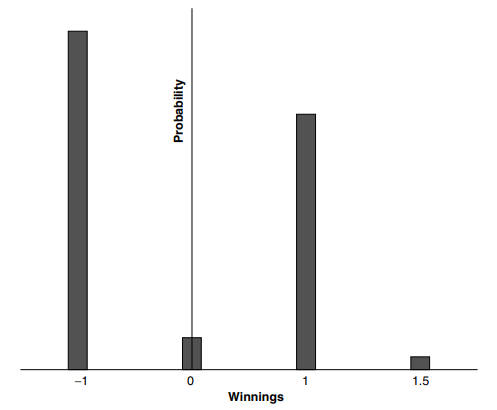
\includegraphics[width=0.65\linewidth]{Imagenes/Parte1/3_Aleatoriedad/blackjack_Dist.png}
    \caption{Distribución de beneficios en el blackjack}
\end{figure}




\subsection{Criterio de Kelly}
Siguiendo con el ejemplo del blackjack, se tiene la v.a.\ $\phi_i$ para denotar el resultado de mano i-ésima, con media $\mu_i$ y desviación típica $\sigma_i$. Suponiendo además que en total incialmente se tiene una cantidad de dinero $P$ y en cada mano se apuesta una fracción $f$ de la cantidad de dinero que se tenga en ese momento. Por lo tanto en la primera mano se obtiene
\[
    P(1+f\phi_1)
\]
en la segunda mano
\[
    P(1+f\phi_1)(1+f\phi_2)
\]
y tras $M$ manos se obtiene
\[
    P\prod_{i=1}^M (1+f\phi_i)
\]
se plantea ahora cómo se elige $f$ para maximiar las ganancias. Si $f$ es muy grande eventualmente se perderá todo (o casi todo el dinero) aunque las expectativas sean positivas (por ejemplo, si se apuesta todo el dinero en una mano); si $f$ es muy es muy pequeño, se ganrá poco y se tardará demasiado en conseguir una cantidad significativa de dinero. Por lo tanto se  busca un valor intermedio.

En este caso se va a elegir $f$ de forma que maximice la \textbf{tasa de crecimiento esperada a largo plazo}, si bien se pueden maximizar con otras estrategias. La tasa de crecimiento es
\[
    \frac{1}{M} \ln\left(  P\prod_{i=1}^M (1+f\phi_i)\right) = \frac{1}{M} \ln(P) + \frac{1}{M} \sum_{i=1}^M \ln(1+f\phi_i)
\]
ignorando el reescalado del primer término y suponiendo que el resultado de cada mano es independiente (no es el caso en el blackjack), su esperanza es:
\begin{align*}
    \mathbb{E}[\ln(1+f\phi_i)] &\overset{\text{(Taylor)}}{=} \mathbb{E}[f\phi_i - \frac{1}{2}f^2\phi_i^2 + O(f^3)] \\
    &= f\mathbb{E}[\phi_i] - \frac{1}{2}f^2\mathbb{E}[\phi_i^2] + O(f^3) \\
    &= f\mu - \frac{1}{2}f^2\sigma^2 + O(f^3)
\end{align*}

Luego, despreciando los términos de orden superior, la tasa de crecimiento esperada a largo plazo es
\begin{align}\label{eq:KellyGrowth}
    f\mu - \frac{1}{2}f^2\sigma^2
\end{align}
que se maximiza cuando
\[
    \boxed{f = \frac{\mu}{\sigma^2}}
\]
dando un crecimiento esperado de
\[
    \frac{\mu}{\sigma^2}\mu - \frac{1}{2}\left(\frac{\mu}{\sigma^2}\right)^2\sigma^2 = \frac{\mu^2}{\sigma^2} - \frac{1}{2}\frac{\mu^2}{\sigma^2} = \boxed{\frac{\mu^2}{2\sigma^2}}
\]
por mano.

Lo importante para obtener ganancias a largo plazo es que la ecuación~\eqref{eq:KellyGrowth} sea positiva:
\begin{align*}
    f\mu - \frac{1}{2}f^2\sigma^2 > 0 \Leftrightarrow f\mu > \frac{1}{2}f^2\sigma^2 \Leftrightarrow \mu > \frac{1}{2}f\sigma^2 \Leftrightarrow \boxed{f < \frac{2\mu}{\sigma^2}}
\end{align*}







\subsection{Apuestas a eventos deportivos: carreras de caballos}
Se tiene en una carrera de caballos $N$ caballos, habiendose apostado una cantidad total $W_i$ sobre el i-ésimo caballo. La casa de apuestas paga $1:q_i$ por el iésimo caballo. Para evitar pérdidas, la casa de apuestas tiene que elegir $q_i$ de forma que nunca pierda.

El total de dinero recaudado antes de la carrera es de
\[
    \sum_{i=1}^N W_i
\]
y si el gana el caballo $j$ la casa de apuestas paga 
\[
    (1+q_j)W_j
\]
luego para conseguir ganancias, lo único de lo que tiene que asegurarse la casa de apuestas es de que
\[
    \sum_{i=1}^N W_i \geq (1+q_j)W_j
\]
es decir que
\[
    \boxed{q_j \leq \frac{\sum_{i=1}^N W_i}{W_j} - 1, \quad \forall j=1,\ldots,N}
\]

Como se puede observar, la probabilidades no tienen nada que ver con las probabilidades reales, si no de lo que se haya apostado.





Ahora desde el punto de vista del apostador, veamos si se puede observar si hay arbitraje. Sea $w_i$ la cantidad apostada al i-ésimo caballo y que el total de dinero apostado es 1, entonces
\[
    \sum_{i=1}^N w_i = 1
\]
y lo que se gana siendo el j-ésimo caballo el ganador es
\[
    (q_j + 1)w_j
\]

El objetivo es por lo tanto encontrar $w_i$ para todo i tal que son todos positivos, suman 1 y la ganancia sea postivia para todo $j$. Por lo tanto, para que haya arbitraje se tiene que conseguir más de 1 (lo invertido):
\begin{align*}
    (q_j + 1)w_j > 1 \Leftrightarrow w_j > \frac{1}{q_j + 1} \\
\end{align*}
leugo el problema es encontrar $w_i$ tal que
\[
    \left\{
    \begin{aligned}\label{eq:ArbitrajeCaballos}
        &\sum_{i=1}^N w_i = 1 \\
        &w_j > \frac{1}{q_j + 1} \quad \forall j
    \end{aligned}
    \right\}
\]
La primera parte implica que la solución debe estar en en plano $\sum_{i=1}^N w_i = 1$ mientras que la segunda dice que para que haya arbitraje el punto $\frac{1}{\vec{q} + 1}$ debe estar por debajo de dicho plano, teniendo en cuenta que todos los valores deben ser positivos. En 2D esto se traduce en la siguiente imagen:
\begin{figure}[H]
    \centering
    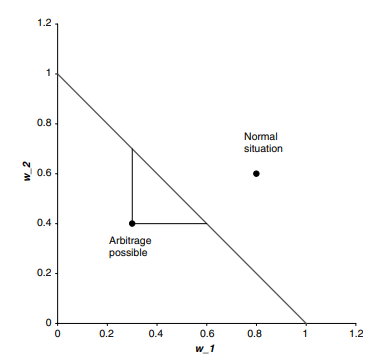
\includegraphics[width=0.65\linewidth]{Imagenes/Parte1/3_Aleatoriedad/Arbitraje_Cabllos.png}
    \caption{Arbitraje en carreras de caballos de dos caballos}
\end{figure}

Una manera rápida de comprobar si hay arbitraje es transformar la ecuacion~\eqref{eq:ArbitrajeCaballos} y comprobar si se cumple:
\[
    1 = \sum_{i=1}^N w_i > \sum_{i=1}^N \frac{1}{q_i + 1} \Rightarrow  \boxed{\sum_{i=1}^N \frac{1}{q_i + 1} < 1}
\]
en caso contrario no hay arbitraje. Una vez comprobado que hay arbitraje, para conseguir ganancias simplemente se debe conseguir un punto $\vec{w}$ dentro de la recta (o plano) $\sum_{i=1}^N w_i = 1$ (comprobando que se cumple la otra condición).





Si no se cumple la condición de arbitraje, existen varias maneras de apostar. Sea $p_i$ la probabilidad de que el i-ésimo caballo gane, entonces se debe cumplir.
\[
    \sum_{i=1}^N p_i = 1
\]
Si se ha apostado en todos los caballos un total de 1, entonces el beneficio o pérdida esperado es
\[
    m = \sum_{i=1}^N p_i w_i (q_i + 1) - 1
\]

Por otro lado, la desviación estandar es
\[
    \sigma = \sqrt{\sum_{i=1}^N p_i( w_i (q_i + 1) - 1 - m)^2}
\]

Existen varias estrategias de apuestas:
\begin{itemize}
    \item \textbf{Maximizar el valor esperado}: en este caso se apuesta todo al caballo con mayor probabilidad de ganar, i.e.\ maximizar $p_i(q_i+1)$. Esta es una apuesta muy arriesgada ya que la esperanza es muy alta pero también la desviación.
    \item \textbf{Minimizar la desviación estándar}: muchas veces se consigue una desviación nula, pero resulta en una esperanza negativa, por lo que no es una buena estrategia.
    \item \textbf{Maximizar rendimiento dividido por desviación estándar}: en este caso se busca un equilibrio entre la esperanza y la desviación $m/\sigma$.
\end{itemize}













\section{Extreme value theory}
Estudia el comportamiento de los valores extremos de una variable aleatoria, es decir, los máximos y mínimos. Se centra en la distribución de los valores extremos, que normalmente con pocas observaciones.

Si $X_i$ son variable identicamente distribuidas (iid) y
\[
    x = \max(X_1, X_2, \ldots, X_n)
\]
entonces la función de distribución de $x$ converge a
\[
    \boxed{F(x) = \exp\left( -\left( 1 + \frac{\xi (x-\mu)}{\sigma} \right)^{-1/\xi} \right)}
\]
donde si $\xi=0$ se tiene la distribución Gumbel, si $\xi > 0$ se tiene la distribución Fréchet y si $\xi < 0$ se tiene la distribución Weibull. En concreto, la de Fréchet es importante en finanzas porque esta asociada a colas pesadas.


Se considera la probabilidad de una pérdida que exceda $u$ por una cantidad $y$, sabiendo que se ha superado $u$, es decir,
\[
    F_u(x) = \mathbb{P}(X - u \leq  y \mid X > u)
\]
Esto se puede aproximar por la Distribución Generalizada de Pareto (GPD):
\[
    \boxed{1 - \left( 1 + \frac{\xi X}{\beta} \right)^{-1/\xi}}
\]

Para colas pesadas, se tiene que $\xi > 0$, en cuyo caso no todos los momentos existen:
\[
    \mathbb{E}[X^k] = \infty, \qquad k \geq \frac{1}{\xi}
\]

Para más información mirar teoría vista en el Athens.







  \clearpage%
  \chapter{Modelación básica de opciones}
  
\section{Modelos Black-Scholes}




\subsection{Modelo opciones básico}
Se construye cartera
\[
\Pi = V(S,t) - \Delta S
\]
sabiendo que
\[
dS = \mu Sdt + \sigma S d\mathnormal{X}
\]
entonces, por el lema de Itô~\ref{Ito} se tiene que
\[
d\Pi = \frac{\partial V}{\partial t}dt + \frac{\partial V}{\partial S}dS + \frac{\sigma^2S^2}{2} \frac{\partial^2 V}{\partial S^2}dt - \Delta dS
\]
que, haciendo un \textbf{delta hedging} $\Delta = \frac{\partial V}{\partial S}$ se obtiene que, sin arbitraje:
\[
d\Pi = \left( \frac{\partial V}{\partial t} + \frac{\sigma^2S^2}{2} \frac{\partial^2 V}{\partial S^2} \right)dt
\]
que debe ser igual que
\[
d\Pi = r\Pi dt = r\left( V - S \frac{\partial V}{\partial S} \right)dt
\]
por lo que
\[
\boxed{\frac{\partial V}{\partial t} + \frac{\sigma^2S^2}{2} \frac{\partial^2 V}{\partial S^2} + rS \frac{\partial V}{\partial S} -rV = 0}
\]

Se debe de tener en cuenta que esto calcula el valor justo de la opción, que es el valor actualizado de su payoff bajo una \textbf{risk-neutral random walk} para el subyacente. Este camino aleatorio es
\[
    dS = rSdt + \sigma S d\mathnormal{X}
\]
Por lo tanto no es lo mismo que la probabilidad de que la opción quede ITM calculada con lo expuesto en el apartado~\ref{sec:ExpectedFirstExitTimes}.


\subsection{Opciones de activos con dividendos continuos}
Tener comprado da un dividendo continuo de $DSdt$, luego la variación de la cartera es
\[
d\Pi = \frac{\partial V}{\partial t}dt + \frac{\partial V}{\partial S}dS + \frac{\sigma^2S^2}{2} \frac{\partial^2 V}{\partial S^2}dt - \Delta dS - D\Delta dS
\]
que usando igualmente que $\Delta = \frac{\partial V}{\partial S}$, se tiene que
\[
\boxed{\frac{\partial V}{\partial t} + \frac{\sigma^2S^2}{2} \frac{\partial^2 V}{\partial S^2} + (r-D)S \frac{\partial V}{\partial S} -rV = 0}
\]



\subsection{Currency options}
En vez de acciones como subyacente, se usa una moneda extranjera con un interés $r_f$ que se comporta como un dividendo continuo, por lo que queda
\[
\boxed{\frac{\partial V}{\partial t} + \frac{\sigma^2S^2}{2} \frac{\partial^2 V}{\partial S^2} + (r-r_f)S \frac{\partial V}{\partial S} -rV = 0}
\]




\subsection{Commodity options}
EL subyacente es un commodity, que tiene un coste de almacenamiento. En este caso se asume continuo $q$ (i.e. $qSdt$). Como es un coste se puede ver como un dividendo negativo, por lo que
\[
\boxed{\frac{\partial V}{\partial t} + \frac{\sigma^2S^2}{2} \frac{\partial^2 V}{\partial S^2} + (r+q)S \frac{\partial V}{\partial S} -rV = 0}
\]




\subsection{Forwards contracts}
Construyendo una cartera igual que BS clásico, se llega a la misma EDP.%
\[
\boxed{\frac{\partial V}{\partial t} + \frac{\sigma^2S^2}{2} \frac{\partial^2 V}{\partial S^2} + rS \frac{\partial V}{\partial S} -rV = 0}
\]
pero se debe añadir como condición final
\[\boxed{V(S,T)=S-\bar{S}}\]
donde $\bar{S}$ es el precio fijado (delivery price). Su solución es
\[
\boxed{S-\bar{S}e^{-r(T-t_0)}}
\]
Su delivery price es el que da valor 0 al contrato en un primer momento, luego 
\[
\bar{S} = S_0e^{r(T-t_0)}
\]
Su forward price, por otro lado, es  
\[
\text{Forward price} = Se^{r(T-t_0)}
\]




\subsection{Future contracts}
Como el valor del contrato se resetea a 0 todos los días (hay compensación diaria), el valor del contrato durante su vida es 0. Denotando por $F(S,t)$ al valor del contrato:
\begin{align*}
    \Pi &= F(S,T) - \Delta S = - \Delta S \\
    d\Pi &= dF(S,T) - d\Delta S \\
    &= \frac{\partial F}{\partial t}dt + \frac{\partial F}{\partial S}dS + \frac{\sigma^2S^2}{2} \frac{\partial^2 F}{\partial S^2}dt - \Delta dS
\end{align*}
luego tomando $\Delta = \frac{\partial F}{\partial S}$ y $d\Pi=r\Pi dt$ se obtiene
\[
\boxed{\frac{\partial F}{\partial t}dt + \frac{\sigma^2S^2}{2} \frac{\partial^2 F}{\partial S^2}dt + rS\frac{\partial F}{\partial S} = 0}
\]
con la condición final de que
\[
\boxed{F(S,T) = S}
\]
Su solución es
\[\boxed{F(S,t) = Se^{r(T-t)}}\]
por lo que para el caso de interés constante, los futures y los forwards valen lo mismo.






\subsection{Opciones sobre futuros}
Son opciones en las que el subyacente es un contrato de futuro. Se sabe que
\[
F = Se^{r(T-t)}
\]
por lo que, haciendo un cambio de variable $V(S,t) = W(F,t)$ se obtiene la EDP
\[
\boxed{\frac{\partial W}{\partial t}dt + \frac{\sigma^2}{2}F^2 \frac{\partial^2 W}{\partial F^2}dt - rW    = 0}
\]




\subsection{Condiciones de frontera y finales}
En una opción europea, se tienen las siguientes condiciones:
\begin{itemize}
    \item Condiciones temporales:
    \begin{itemize}
        \item Call:
        \[\boxed{C(S,T) = \max(S-E, 0)}\]
        \item Put:
        \[\boxed{C(S,T) = \max(E-S, 0)}\]
    \end{itemize}
    \item Condiciones de frontera: (se justificarán más adelante)
    \begin{itemize}
        \item Call:
        \[\boxed{C(0,t) = 0}\]
        \[\boxed{C(S,t) \xrightarrow{S\rightarrow\infty}  S - Ee^{-r(T-t)}}\]
        \item Put:
        \[\boxed{P(0,t) = Ee^{-r(T-t)}}\]
        \[\boxed{P(S,t) \xrightarrow{S\rightarrow\infty}  0}\]
    \end{itemize}
\end{itemize}






\subsection{Algunas propiedades de las opciones europeas}

\begin{remark}\label{ActPayoff}
    Si el payoff de una cartera es mayor o igual a $M$, entonces, en ausencia de arbitraje, el valor actual de la cartera es mayor o igual que el valor actualizado:
    \[\boxed{\Pi(T) \geq M \Rightarrow \Pi(t) \geq Me^{-r(T-t)}}\]
    Si no fuese el caso, se podría pedir al banco una cantidad $Me^{-r(T-t)}$ en tiempo $t$ y comprar la cartera. Entonces, en tiempo $T$ se pagaría el préstamo con el payoff y se generaría beneficio.
\end{remark}


\begin{proposition}\label{PropsCall}
    Sea $C(S,t)$ una opción Call europea con fecha de ejercicio $T$ y subyacente $S$ sin dividendos; entonces, en ausencia de arbitraje:
    \begin{enumerate}
        \item $\boxed{C \leq S}$
        \item $\boxed{C \geq \max(S-Ee^{-r(T-t)}, 0)}$
        \item $\boxed{0 \leq C_1 -C_2 \leq (E_2-E_1)e^{-r(T-t)}$ con $E_1<E_2}$.
    \end{enumerate}
\end{proposition}
\begin{proof}
    Utilizando la observación~\ref{ActPayoff}:
    \begin{enumerate}
        \item Sea la cartea $\Pi = S-C$, entonces
        \begin{align*}
            \Pi(T) &= S - \max(S - E,0) \\
            &= \left\{
            \begin{array}{ll}
              S,       & 0 \leq S \leq E \\
              E,        & S \geq E
            \end{array}
            \right\} \geq 0 \xRightarrow{\ref{ActPayoff}} \\
            \xRightarrow{\ref{ActPayoff}} \Pi(t) &= S-C \geq 0 \Rightarrow \\
            \Rightarrow S &\geq 0
        \end{align*}
        \item Sea la cartea $\Pi = S-C$, entonces
        \begin{align*}
            \Pi(T) &= S - \max(S - E,0) \\
            &= \left\{
            \begin{array}{ll}
              S,       & 0 \leq S \leq E \\
              E,        & S \geq E
            \end{array}
            \right\} \leq E \xRightarrow{\ref{ActPayoff}}\\
            \xRightarrow{\ref{ActPayoff}} \Pi(t) &= S - C \leq Ee^{-r(T-t)} \\
            \Rightarrow C &\geq  S - Ee^{-r(T-t)} \xRightarrow{C \geq 0} \\
            \xRightarrow{C \geq 0} C &\geq \max(S - Ee^{-r(T-t)}, 0)
        \end{align*}
        \item Sea la cartea $\Pi = C_1 - C_2$, entonces
        \begin{align*}
            \Pi(T) &= \max(S - E_1,0) - \max(S - E_2,0) \\
            &= \left\{
            \begin{array}{ll}
            0,       & 0 \leq S < E_1 \\
            S-E_1,   & E_1 \leq S < E_2 \\
            E_2-E_1, & S \geq E_2
            \end{array}
            \right\} \Rightarrow \\
            0 &\leq \Pi(T) \leq E_2-E_1 \xRightarrow{\ref{ActPayoff}}\\
            \xRightarrow{\ref{ActPayoff}} 0 &\leq \Pi(t) \leq (E_2-E_1)e^{-r(T-t)} \Rightarrow \\
            \Rightarrow 0 &\leq C_1 - C_2 \leq (E_2-E_1)e^{-r(T-t)}
        \end{align*}
    \end{enumerate}
\end{proof}




\begin{proposition}
    Sea $P(S,t)$ una opción Put europea con fecha de ejercicio $T$ y subyacente $S$ sin dividendos; entonces, en ausencia de arbitraje:
    \begin{enumerate}
        \item $\boxed{P \leq Ee^{-r(T-t)}}$
        \item $\boxed{P \geq Ee^{-r(T-t)} - S}$
        \item $\boxed{0 \leq P_2 - P_1 \leq (E_2-E_1)e^{-r(T-t)}$ con $E_1<E_2}$.
    \end{enumerate}
\end{proposition}
\begin{proof}
    Utilizando la observación~\ref{ActPayoff}:
    \begin{enumerate}
        \item Sea la cartea $\Pi = P - E$, entonces
        \begin{align*}
            \Pi(T) &= \max(E - S,0) - E \\
            &= \left\{
            \begin{array}{ll}
              -S,       & 0 \leq S < E \\
              -E,        & S \geq E
            \end{array}
            \right\} \leq 0 \xRightarrow{\ref{ActPayoff}}\\
            \xRightarrow{\ref{ActPayoff}} \Pi(t) &= P - Ee^{-r(T-t)} \leq 0 \\
            \Rightarrow P &\leq  Ee^{-r(T-t)}
        \end{align*}
        \item Sea la cartea $\Pi = S + P$, entonces
        \begin{align*}
            \Pi(T) &= S +\max(E - S,0) \\
            &= \left\{
            \begin{array}{ll}
              E,       & 0 \leq S < E \\
              S,        & S \geq E
            \end{array}
            \right\} \geq E \xRightarrow{\ref{ActPayoff}}\\
            \xRightarrow{\ref{ActPayoff}} \Pi(t) &= S + P \geq Ee^{-r(T-t)} \\
            \Rightarrow P &\geq  Ee^{-r(T-t)} - S
        \end{align*}
        \item Sea la cartea $\Pi = P_2 - P_1$, entonces
        \begin{align*}
            \Pi(T) &= \max(E_2 - S,0) - \max(E_1 - S,0) \\
            &= \left\{
            \begin{array}{ll}
              E_2 - E_1,       & 0 \leq S < E_1 \\
              E_2-S,        & E_1 \leq S < E_2 \\
              0,        & S \geq E_2
            \end{array}
            \right\} \Rightarrow \\
            0 &\leq \Pi(T) \leq E_2-E_1 \xRightarrow{\ref{ActPayoff}}\\
            \xRightarrow{\ref{ActPayoff}} 0 &\leq \Pi(t) \leq (E_2-E_1)e^{-r(T-t)} \Rightarrow \\
            \Rightarrow 0 &\leq P_2-P_1 \leq (E_2-E_1)e^{-r(T-t)}
        \end{align*}
    \end{enumerate}
\end{proof}





\begin{proposition}
    Sea $P(S,t)$ una opción Put europea con fecha de ejercicio $T$ y subyacente $S$ sin dividendos; entonces, en ausencia de arbitraje:
    \begin{enumerate}
        \item $\boxed{C_A \geq C_B}$ donde $C_a, C_B$ son Calls europeas con precio de ejercicio $E$ y fechas de ejercicio $T_A, T_B$ tal que $T_A > T_B$.
        \item $\boxed{C_2 \leq \frac{E_3-E_2}{E_3-E_1}C_1 + \frac{E_2-E_1}{E_3-E_1}C_3}$ donde $C_1, C_2, C_3$ son Calls europeas con fecha de ejercicio $T$ y strikes $E_1, E_2, E_3$ donde $E_1<E_2<E_3$.
    \end{enumerate}
\end{proposition}
\begin{proof}
    Utilizando la observación~\ref{ActPayoff}:
    \begin{enumerate}
        \item Sea la cartera $\Pi = C_A-C_B$, entonces
        \begin{align*}
            \Pi(T_B) &= C_A(S,T_B) - \max(S-E,0) \overset{\ref{PropsCall}}{\geq} \\
            &\overset{\ref{PropsCall}}{\geq} \max(S-Ee^{-r(T-t)}) - \max(S-E,0) \geq \\
            &\geq \max(S-E) - \max(S-E,0) = 0 \\
            &\Rightarrow \Pi(T_B) \geq 0 \Rightarrow \\
            &\Rightarrow \Pi(t) = C_A-C_B \geq 0 \Rightarrow \\
            &\Rightarrow C_A \geq C_B
        \end{align*}
        \item Sea la cartera $\Pi = - C_2 + \lambda C_1 + (1-\lambda) C_3 $ y se considera 
        \begin{align*}
            &E_2 = \lambda E_1 + (1-\lambda) E_3 = \lambda E_1 + E_3-\lambda E_3 = E_3 + \lambda(E_1-E_3) \Rightarrow \\
            \Rightarrow &\lambda = \frac{E_2-E_3}{E_1-E_3} = \frac{E_3-E_2}{E_3-E_1} \Rightarrow \\
            \Rightarrow &(1-\lambda) = \frac{E_2-E_1}{E_3-E_1}
        \end{align*}
        entonces
        \begin{align*}
            \Pi(T) &= -\max(S-E_2, 0) + \lambda\max(S-E_1,0) + (1+\lambda)\max(S-E_3, 0) = \\
            &=\left\{
            \begin{array}{ll}
              0,       & 0 \leq S < E_1 \\
              \lambda(S-E_1),        & E_1 \leq S < E_2 \\
              - (S-E_2) +\lambda(S-E_1),        & E_2 \leq S < E_3 \\
              - (S-E_2) +\lambda(S-E_1) + (1-\lambda)(S-E_3),        & S \geq E_3
            \end{array}
            \right\} \\
            &=\left\{
            \begin{array}{ll}
              0,       & 0 \leq S < E_1 \\
              \frac{E_3-E_2}{E_3-E_1}(S-E_1),        & E_1 \leq S < E_2 \\
              (1-\lambda)(E_3+S),        & E_2 \leq S < E_3 \\
              (1-\lambda)(E_3+S) + (1-\lambda)(S-E_3),        & S \geq E_3
            \end{array}
            \right\} \\
            &=\left\{
            \begin{array}{ll}
              0,       & 0 \leq S < E_1 \\
              \lambda(S-E_1),        & E_1 \leq S < E_2 \\
              (1-\lambda)(E_3+S),        & E_2 \leq S < E_3 \\
              (1-\lambda)2S,        & S \geq E_3
            \end{array}
            \right\} \\
            &=\left\{
            \begin{array}{ll}
              0,       & 0 \leq S < E_1 \\
              \frac{E_3-E_2}{E_3-E_1}(S-E_1),        & E_1 \leq S < E_2 \\
              \frac{E_2-E_1}{E_3-E_1}(E_3+S),        & E_2 \leq S < E_3 \\
              \frac{E_2-E_1}{E_3-E_1}2S,        & S \geq E_3
            \end{array}
            \right\} \geq 0 \xRightarrow{\ref{ActPayoff}} \\
            \xRightarrow{\ref{ActPayoff}} \Pi(t) &= - C_2 + \lambda C_1 + (1-\lambda) C_3 \geq 0 \\
            C_2 &\geq \frac{E_3-E_2}{E_3-E_1} C_1 + \frac{E_2-E_1}{E_3-E_1} C_3
        \end{align*}
    \end{enumerate}
\end{proof}








  \newpage
  
\section{Comportamiento de las EDPs}

\subsection{Significado de los términos de una EDP}
Sea una EDP de la siguiente forma:
$$\frac{\partial u}{\partial t} + c(u) \frac{\partial u}{\partial x} = D(u) \frac{\partial^2 u}{\partial x^2} + R(u)$$
entonces se tienen los siguientes términos:
\begin{itemize}
    \item \textbf{Término de difusión} ($D(u) \frac{\partial^2 u}{\partial x^2}$): es el responsable de disipar o concentrar la solución . Si $D(u)>0$ entonces la solución se suaviza mientras que $D(u)<0$ hace que la solución se concentre. 
    \item \textbf{Término de convección} ($c(u) \frac{\partial u}{\partial x}$): representa el transporte con velocidad $c(u)$ hacia la derecha si $c(u)>0$ o hacia la izquierda si $c(u)<0$.
    \item \textbf{Término de reacción} ($R(u)$): representa la salida o entrada local de $u$. Se puede ver como crear/eliminar masa (fuentes o sumideros).
\end{itemize}

Sabiendo que la EDP de Black-Scholes clásica es
$$\frac{\partial V}{\partial t} + \frac{\sigma^2S^2}{2} \frac{\partial^2 V}{\partial S^2} + rS \frac{\partial V}{\partial S} -rV = 0 $$
entonces:
\begin{itemize}
    \item El término de \textbf{difusión} $\frac{\sigma^2}{2}S^2 > 0$ indica que la solución se suaviza y que los picos se homogeinizan.
    \item El término de \textbf{convección} $rS > 0$ indica que el resultado se mueve hacia los valores de $S$ positivos (hacia la derecha).
    \item El término de \textbf{reacción} $rV > 0$ indica un decaimiento general del valor de la opción a medida que pasa el tiempo.
\end{itemize}














  \newpage
  
\section{Soluciones y griegas}


\subsection{Griegas}
\begin{center}
    \begin{tabularx}{\textwidth}{|c|X|}
        \hline
        \textbf{Delta} $\Delta = \frac{\partial V}{\partial S}$ & Lo que se tiene que comprar/vender en cada momento según el valor del subyacente para mantener la cartera libre de riesgo. \\
        \hline
        \textbf{Gamma} $\Gamma = \frac{\partial^2 V}{\partial S^2}$ & Es una medida de cuánto y cuantas veces se tiene que \textit{rehedged} para mantener la cartera libre de riesgo. \\
        \hline
        \textbf{Theta} $\Theta = \frac{\partial V}{\partial t}$ & Contribuye a que la cartera gane el interés correspondiente. \\
        \hline
        \textbf{Speed} $\frac{\partial^3 V}{\partial S^3}$ & Como gamma, pero para mayor precisión. \\
        \hline
        \textbf{Vega} $\frac{\partial V}{\partial \sigma}$ & Variación con respecto a la volatilidad del subyacente. \\
        \hline
        \textbf{Rho} $\frac{\partial V}{\partial r}$ & Sensibilidad de la opción a cambios en la tasa de interés. En la práctica se usa la estructura temporal completa de tasas. \\
        \hline
    \end{tabularx}
\end{center}
Sabiendo la \textit{call-put parity} $C(S,t)-P(S,t)=S-Ee^{-r(T-t)}$, las relaciones entre las griegas en opciones europeas Call y Put son:
\begin{itemize}
    \item \textbf{Delta}: $\boxed{\Delta_{Call} = 1 + \Delta_{Put}}$
    \item \textbf{Gamma}: $\boxed{\Gamma_{Call} = \Gamma_{Put}}$
    \item \textbf{Theta}: $\boxed{\Theta_{Call} = \Theta_{Put} - rEe^{-r(T-t)}}$
    \item \textbf{Vega}: $\boxed{\nu_{Call} = \nu_{Put}}$
    \item \textbf{Rho}: $\boxed{\rho_{Call} = \rho_{Put} + E(T-t)e^{-r(T-t)}}$
\end{itemize}



\subsection{Tablas de soluciones}
\begin{center}
    \begin{tabularx}{\textwidth}{|X|X|X|}
        \hline
         & \textbf{Call} & \textbf{Put} \\
         \hline
         \textbf{Value (Black-Scholes value)} &  $S e^{-D(T-t)} N(d_1) - E e^{-r(T-t)} N(d_2)$  &  $-S e^{-D(T-t)} N(-d_1) + E e^{-r(T-t)} N(-d_2)$  \\
         \hline
         \textbf{Delta } $\left( \frac{\partial V}{\partial S} \right)$ & $ e^{-D(T-t)} N(d_1) $ & $ e^{-D(T-t)} (N(d_1) - 1) $ \\
         \hline
        \textbf{Gamma } $\left( \frac{\partial^2 V}{\partial S^2} \right)$ & \multicolumn{2}{c|}{$ \frac{e^{-D(T-t)} N'(d_1)}{\sigma S \sqrt{T - t}} $} \\
        \hline
        \textbf{Theta } $\left( \frac{\partial V}{\partial t} \right)$ & $ -\frac{\sigma S e^{-D(T-t)} N'(d_1)}{2 \sqrt{T - t}} + D S N(d_1) e^{-D(T-t)} - r E e^{-r(T-t)} N(d_2) $ & $ -\frac{\sigma S e^{-D(T-t)} N'(-d_1)}{2 \sqrt{T - t}} - D S N(-d_1) e^{-D(T-t)} + r E e^{-r(T-t)} N(-d_2) $ \\
        \hline
        \textbf{Speed } $\left( \frac{\partial^3 V}{\partial S^3} \right)$ & \multicolumn{2}{c|}{$ -\frac{e^{-D(T-t)} N'(d_1)}{\sigma^2 S^2 (T - t)} (d_1 + \sigma \sqrt{T - t}) $} \\
        \hline
        \textbf{Vega } $\left( \frac{\partial V}{\partial \sigma} \right)$ & \multicolumn{2}{c|}{$ S \sqrt{T - t} e^{-D(T-t)} N'(d_1) $} \\
        \hline
        \textbf{Rho } $\left( \frac{\partial V}{\partial r} \right)$ & $ E (T - t) e^{-r(T-t)} N(d_2) $ & $ -E (T - t) e^{-r(T-t)} N(-d_2) $ \\
        \hline
        \textbf{Rho } $\left( \frac{\partial V}{\partial D} \right)$ & $ -(T - t) S e^{-D(T-t)} N(d_1) $ & $ (T - t) S e^{-D(T-t)} N(-d_1) $ \\
        \hline
    \end{tabularx}\label{tab:soluciones_BS_europeas}
\end{center}
\begin{align}
    d_1 &= \frac{\log \left( \frac{S}{E} \right) + \left( r - D + \frac{1}{2} \sigma^2 \right) (T - t)}{\sigma \sqrt{T - t}} && N(x) = \frac{1}{\sqrt{2 \pi}} \int_{-\infty}^x e^{- \frac{1}{2} y^2} \, dy \\
    d_2 &= d_1 - \sigma \sqrt{T - t} &&  N'(x) = \frac{1}{\sqrt{2 \pi}} e^{- \frac{1}{2} x^2}
\end{align}\label{eq:d_sol_BS}

\begin{center}
    \begin{tabularx}{\textwidth}{|X|X|X|}
        \hline
        & \textbf{Binary Call} & \textbf{Binary Put} \\
        \hline
        \textbf{Value (Black-Scholes value)} & $ e^{-r(T-t)} N(d_2) $ & $ e^{-r(T-t)} (1 - N(d_2)) $ \\
        \hline
        \textbf{Delta } & $ \frac{e^{-r(T-t)} N'(d_2)}{\sigma S \sqrt{T - t}} $ & $ -\frac{e^{-r(T-t)} N'(d_2)}{\sigma S \sqrt{T - t}} $ \\
        \hline
        \textbf{Gamma } $\left( \frac{\partial^2 V}{\partial S^2} \right)$ & $ -\frac{e^{-r(T-t)} d_1 N'(d_2)}{\sigma^2 S (T - t)} $ & $ \frac{e^{-r(T-t)} d_1 N'(d_2)}{\sigma^2 S (T - t)} $ \\
        \hline
        \textbf{Theta } $\left( \frac{\partial V}{\partial t} \right)$ & $ r e^{-r(T-t)} N(d_2) \left( \frac{d_1}{2 (T - t)} - \frac{r - D}{\sigma \sqrt{T - t}} \right) $ & $ r e^{-r(T-t)} (1 - N(d_2)) \left( \frac{d_1}{2 (T - t)} - \frac{r - D}{\sigma \sqrt{T - t}} \right) $ \\
        \hline
        \textbf{Speed } $\left( \frac{\partial^3 V}{\partial S^3} \right)$ & \multicolumn{2}{c|}{$ \frac{e^{-r(T-t)} N'(d_2)}{\sigma^3 S^3 (T - t)} \left( -2 d_1 + \frac{1 - d_1 d_2}{\sigma \sqrt{T - t}} \right) $} \\
        \hline
        \textbf{Vega } $\left( \frac{\partial V}{\partial \sigma} \right)$ & $ -\frac{e^{-r(T-t)} N'(d_2) d_1}{\sigma \sqrt{T - t}} $ & $ \frac{e^{-r(T-t)} N'(d_2) d_1}{\sigma \sqrt{T - t}} $ \\
        \hline
        \textbf{Rho } $\left( \frac{\partial V}{\partial r} \right)$ & $ -(T - t) e^{-r(T-t)} N(d_2) + \frac{\sqrt{T-t}}{\sigma}e^{-r(T-t)} N'(d_2) $ & $ -(T - t) e^{-r(T-t)} (1 - N(d_2)) - \frac{\sqrt{T-t}}{\sigma}e^{-r(T-t)} N'(d_2) $ \\
        \hline
        \textbf{Rho } $\left( \frac{\partial V}{\partial D} \right)$ & $ \frac{\sqrt{T - t}}{\sigma} e^{-r(T-t)} N'(d_2) $ & $ -\frac{\sqrt{T - t}}{\sigma} e^{-r(T-t)} N'(d_2) $ \\
        \hline
    \end{tabularx}
\end{center}
\begin{align*}
    d_1 &= \frac{\log \left( \frac{S}{E} \right) + \left( r - D + \frac{1}{2} \sigma^2 \right) (T - t)}{\sigma \sqrt{T - t}} && N(x) = \frac{1}{\sqrt{2 \pi}} \int_{-\infty}^x e^{- \frac{1}{2} y^2} \, dy \\
    d_2 &= d_1 - \sigma \sqrt{T - t} &&  N'(x) = \frac{1}{\sqrt{2 \pi}} e^{- \frac{1}{2} x^2}
\end{align*}




\subsection{Representación gráfica de soluciones}
En este apartado se va a graficar cada una de las soluciones
\subsubsection{Call option}
\begin{figure}[H]
    \centering
    \begin{subfigure}[b]{0.35\linewidth}
        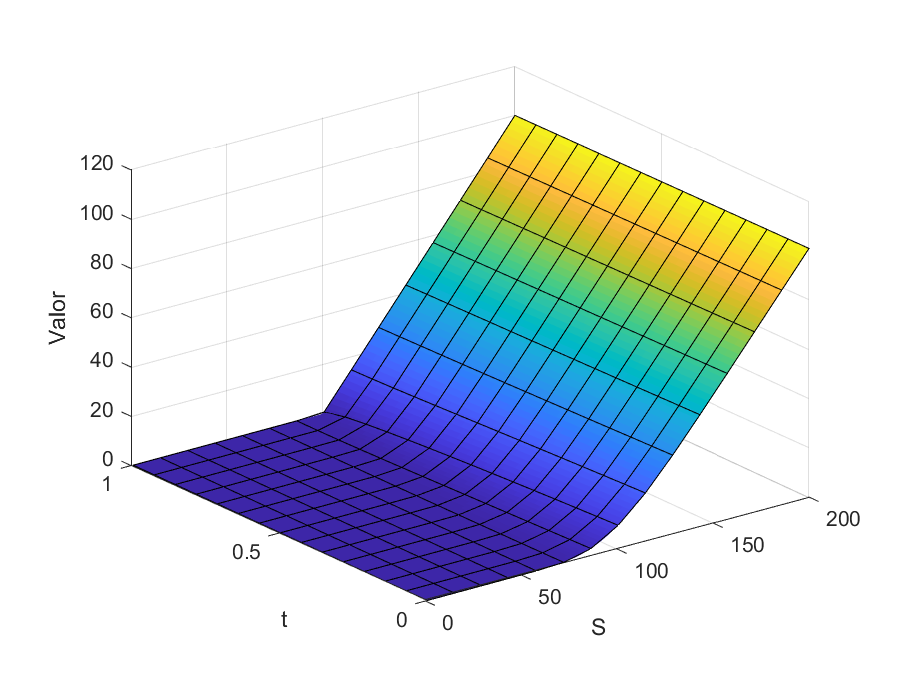
\includegraphics[width=\linewidth]{Imagenes/Parte1/6_Sols/Call/Call3D.eps}
        \caption{Solución}
    \end{subfigure}
    \begin{subfigure}[b]{0.35\linewidth}
        \includegraphics[width=\linewidth]{Imagenes/Parte1/6_Sols/Call/CallSFijo.eps}
        \caption{Solución con S fijo}
    \end{subfigure}
    \begin{subfigure}[b]{0.35\linewidth}
        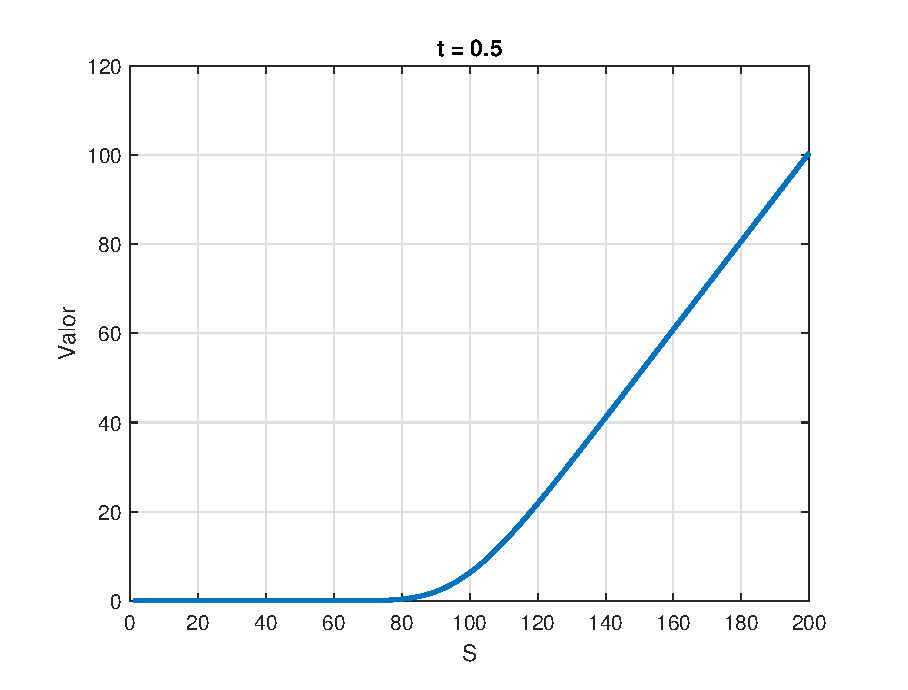
\includegraphics[width=\linewidth]{Imagenes/Parte1/6_Sols/Call/CalltFIjo.eps}
        \caption{Solución con t fijo}
    \end{subfigure}
    \begin{subfigure}[b]{0.35\linewidth}
        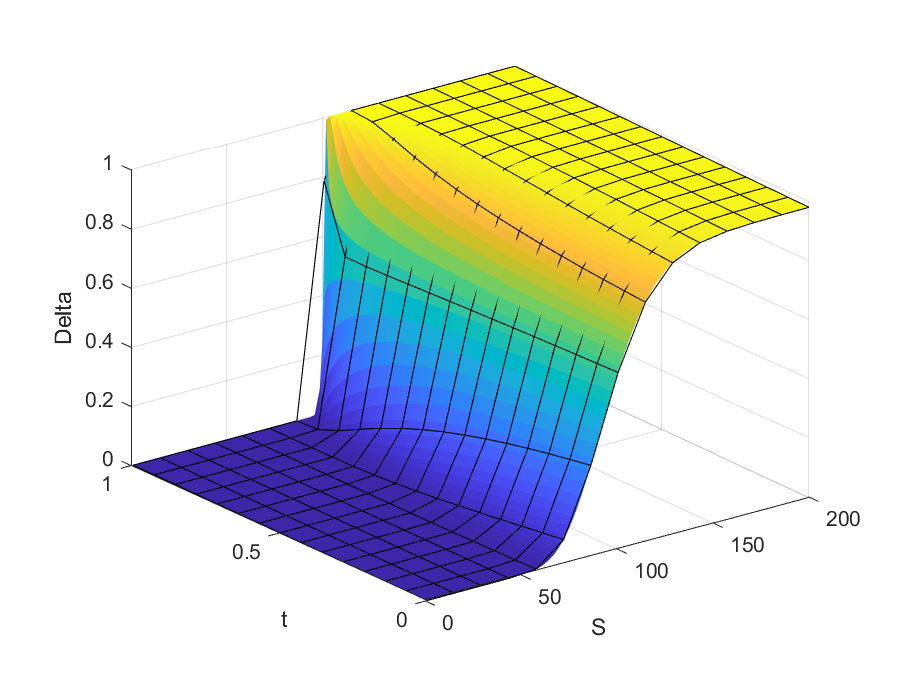
\includegraphics[width=\linewidth]{Imagenes/Parte1/6_Sols/Call/Call_Delta.eps}
        \caption{Delta}
    \end{subfigure}
    \begin{subfigure}[b]{0.35\linewidth}
        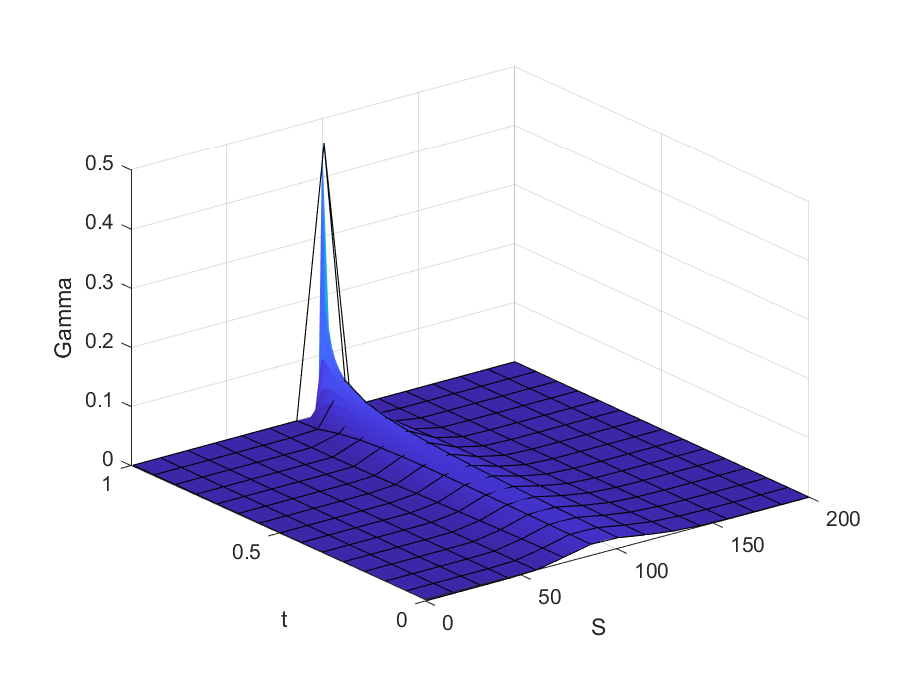
\includegraphics[width=\linewidth]{Imagenes/Parte1/6_Sols/Call/Call_Gamma.eps}
        \caption{Gamma}
    \end{subfigure}
    \begin{subfigure}[b]{0.35\linewidth}
        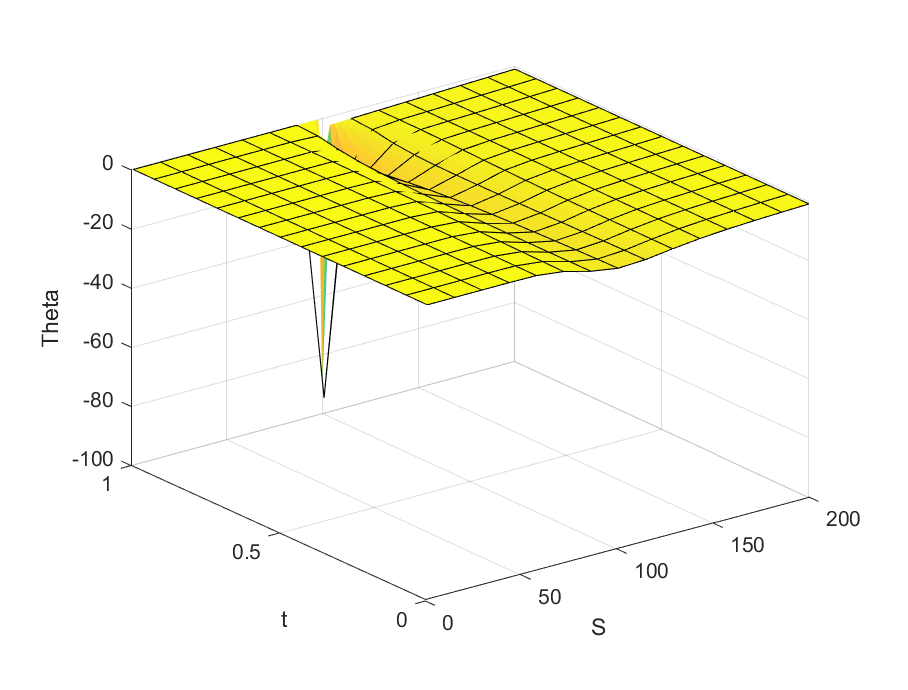
\includegraphics[width=\linewidth]{Imagenes/Parte1/6_Sols/Call/Call_Theta.eps}
        \caption{Theta}
    \end{subfigure}
    \begin{subfigure}[b]{0.35\linewidth}
        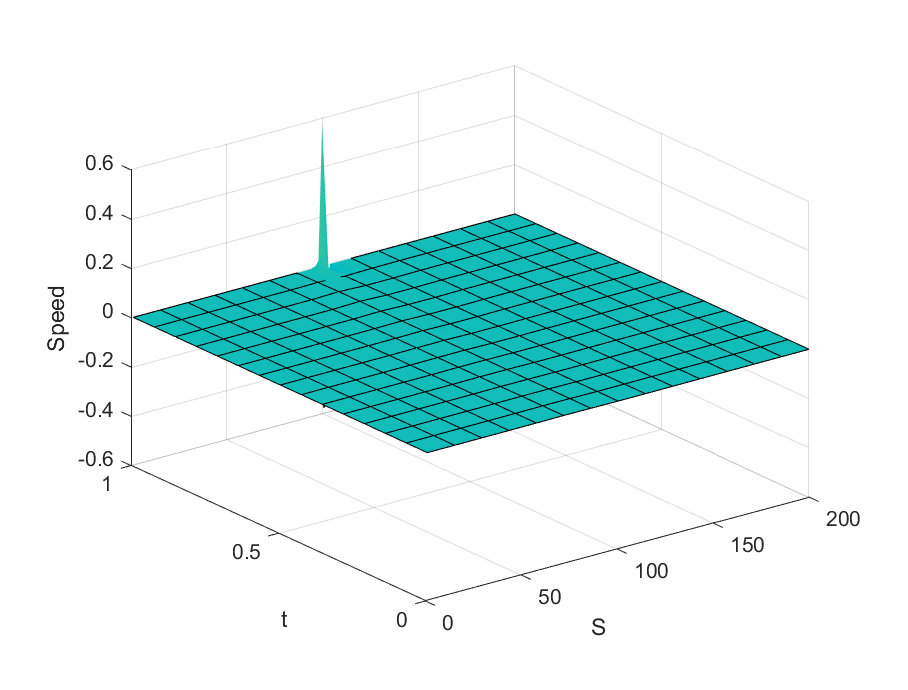
\includegraphics[width=\linewidth]{Imagenes/Parte1/6_Sols/Call/Call_Speed.eps}
        \caption{Speed}
    \end{subfigure}
    \begin{subfigure}[b]{0.35\linewidth}
        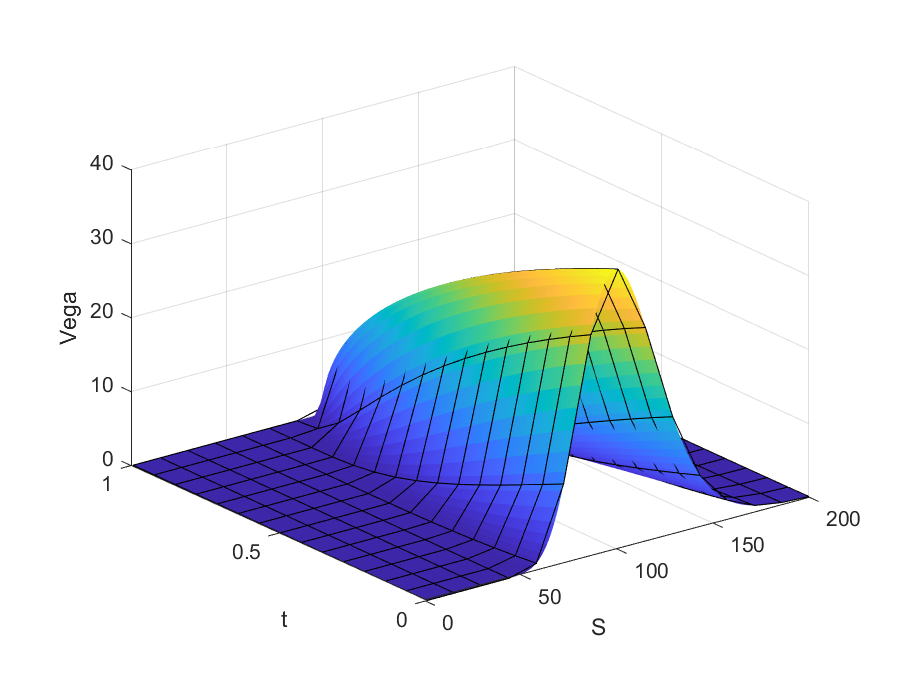
\includegraphics[width=\linewidth]{Imagenes/Parte1/6_Sols/Call/Call_Vega.eps}
        \caption{Vega}
    \end{subfigure}
    \begin{subfigure}[b]{0.35\linewidth}
        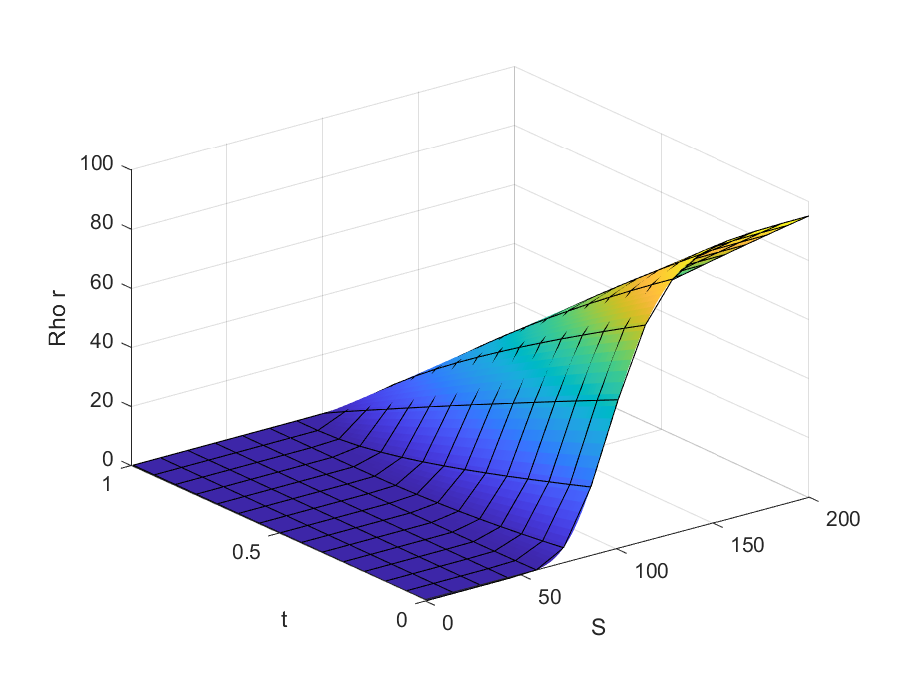
\includegraphics[width=\linewidth]{Imagenes/Parte1/6_Sols/Call/Call_Rho_r.eps}
        \caption{Rho (r)}
    \end{subfigure}
    \begin{subfigure}[b]{0.35\linewidth}
        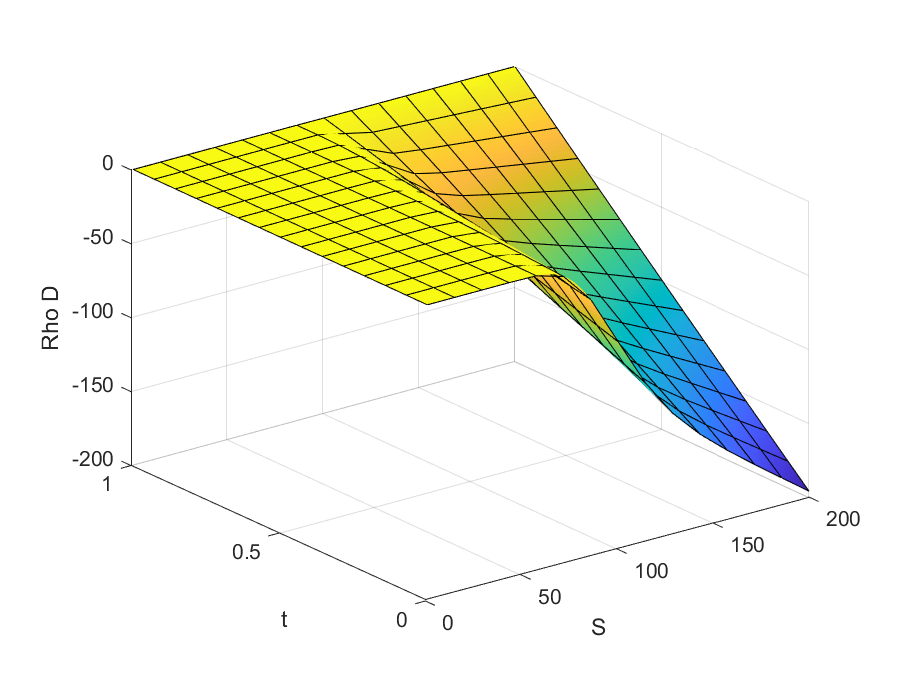
\includegraphics[width=\linewidth]{Imagenes/Parte1/6_Sols/Call/Call_Rho_D.eps}
        \caption{Rho (D)}
    \end{subfigure}
\end{figure}


\subsubsection{Put option}
\begin{figure}[H]
    \centering
    \begin{subfigure}[b]{0.35\linewidth}
        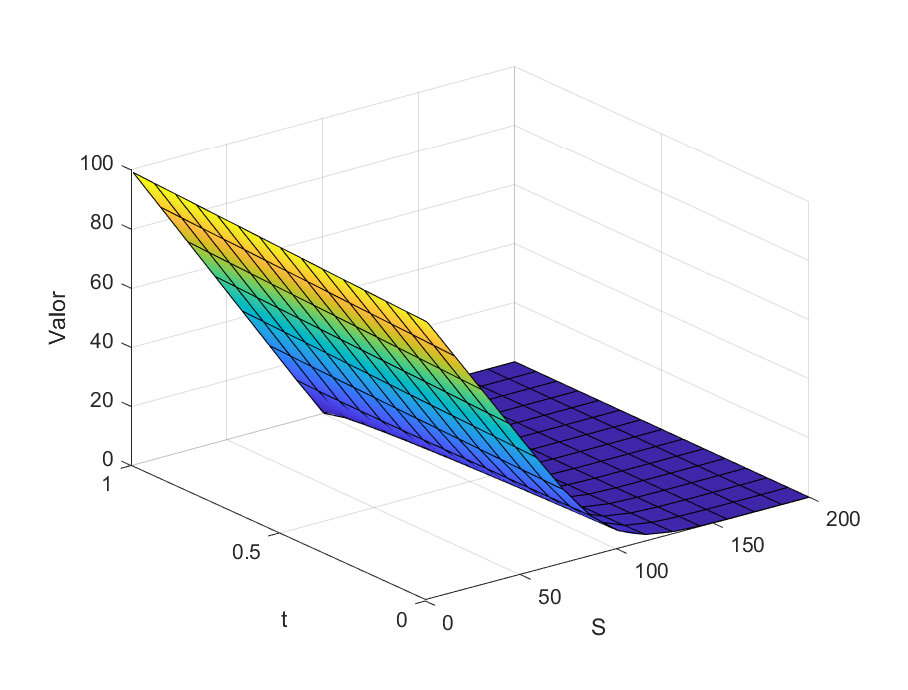
\includegraphics[width=\linewidth]{Imagenes/Parte1/6_Sols/Put/Put3D.eps}
        \caption{Solución}
    \end{subfigure}
    \begin{subfigure}[b]{0.35\linewidth}
        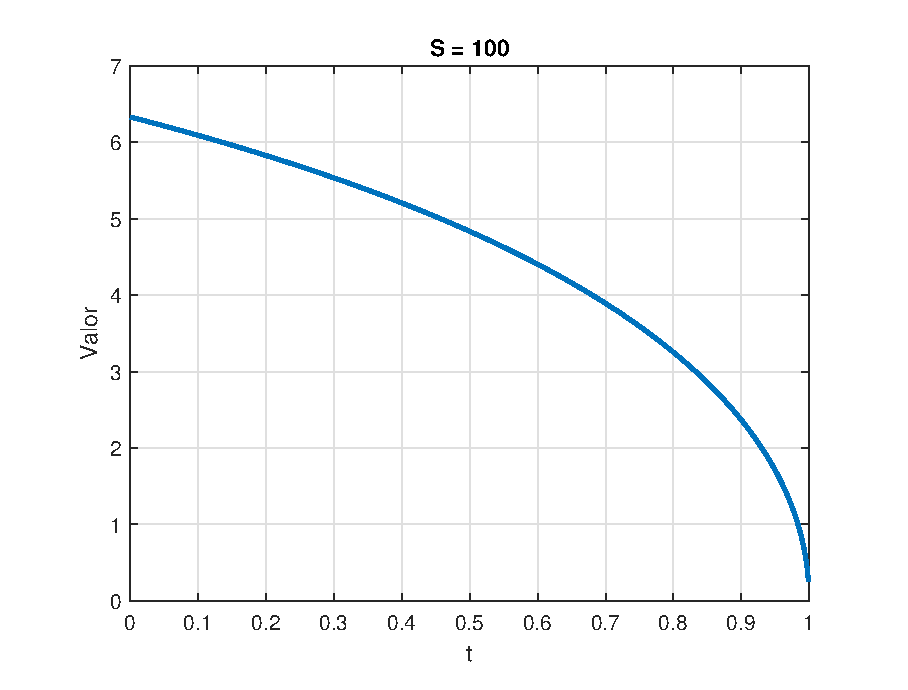
\includegraphics[width=\linewidth]{Imagenes/Parte1/6_Sols/Put/PutSFijo.eps}
        \caption{Solución con S fijo}
    \end{subfigure}
    \begin{subfigure}[b]{0.35\linewidth}
        \includegraphics[width=\linewidth]{Imagenes/Parte1/6_Sols/Put/PuttFIjo.eps}
        \caption{Solución con t fijo}
    \end{subfigure}
    \begin{subfigure}[b]{0.35\linewidth}
        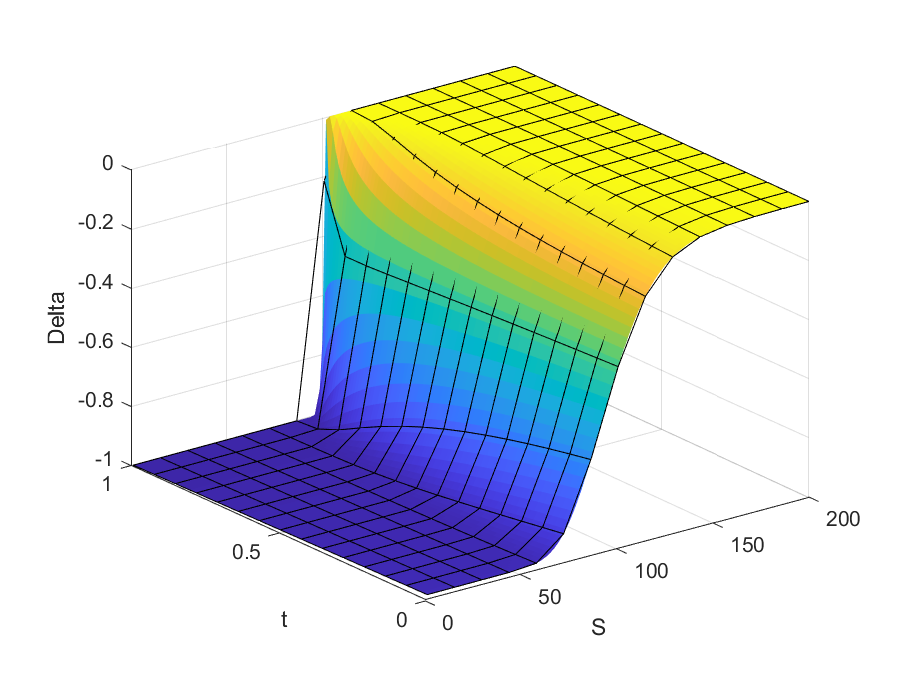
\includegraphics[width=\linewidth]{Imagenes/Parte1/6_Sols/Put/Put_Delta.eps}
        \caption{Delta}
    \end{subfigure}
    \begin{subfigure}[b]{0.35\linewidth}
        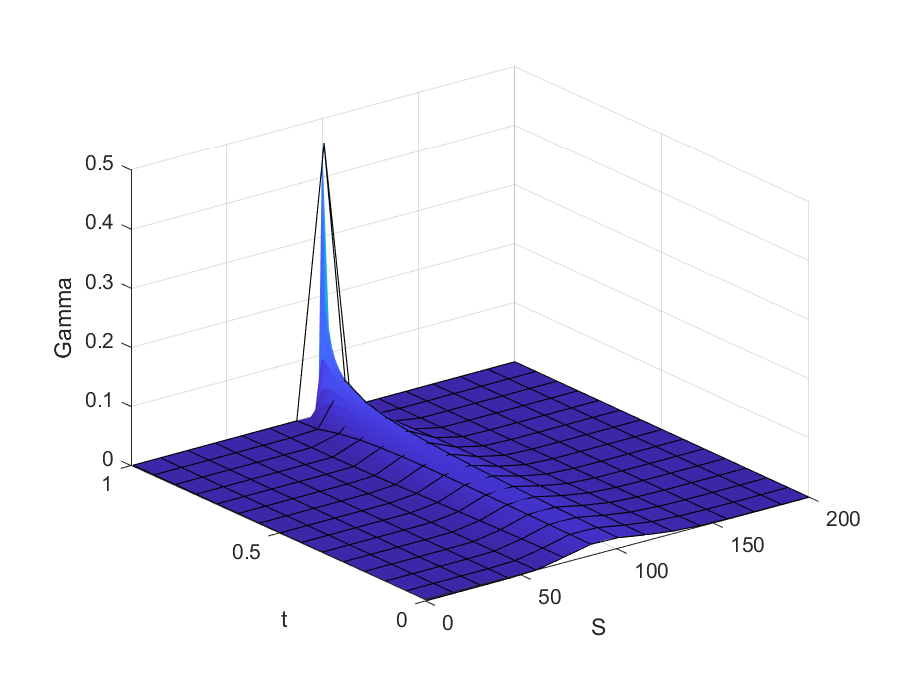
\includegraphics[width=\linewidth]{Imagenes/Parte1/6_Sols/Put/Put_Gamma.eps}
        \caption{Gamma}
    \end{subfigure}
    \begin{subfigure}[b]{0.35\linewidth}
        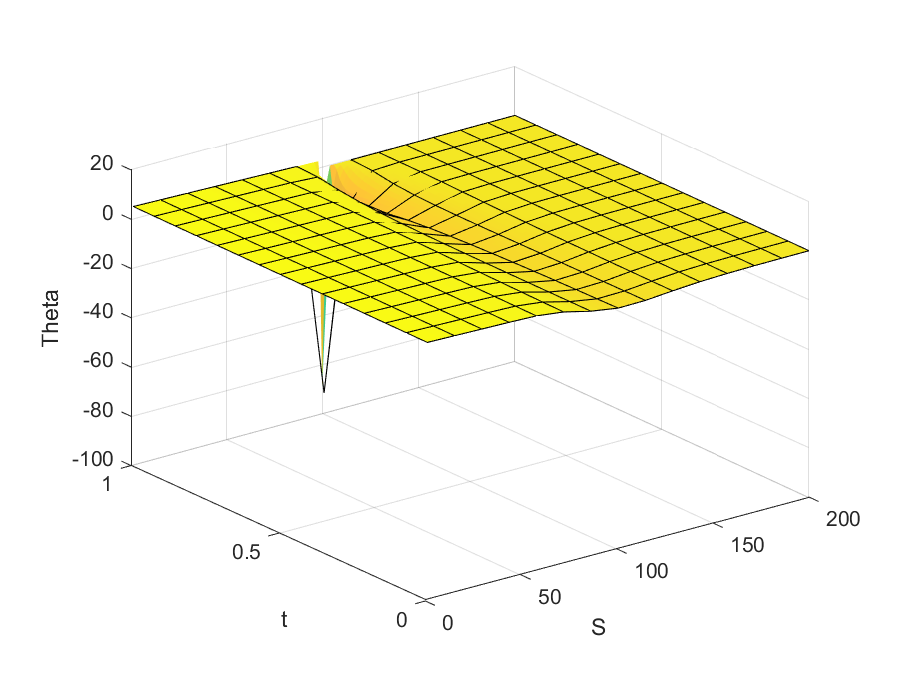
\includegraphics[width=\linewidth]{Imagenes/Parte1/6_Sols/Put/Put_Theta.eps}
        \caption{Theta}
    \end{subfigure}
    \begin{subfigure}[b]{0.35\linewidth}
        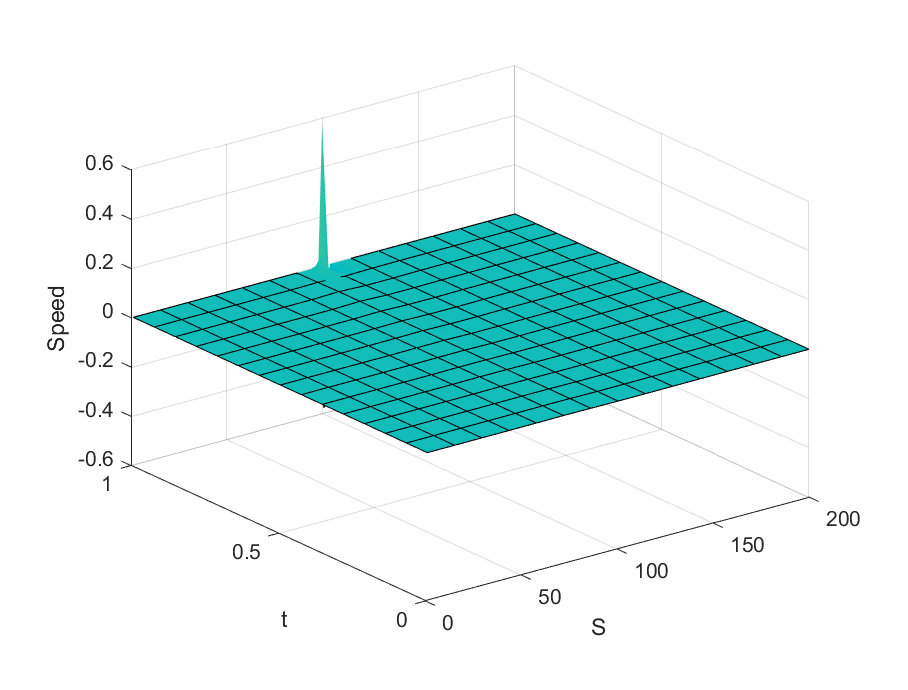
\includegraphics[width=\linewidth]{Imagenes/Parte1/6_Sols/Put/Put_Speed.eps}
        \caption{Speed}
    \end{subfigure}
    \begin{subfigure}[b]{0.35\linewidth}
        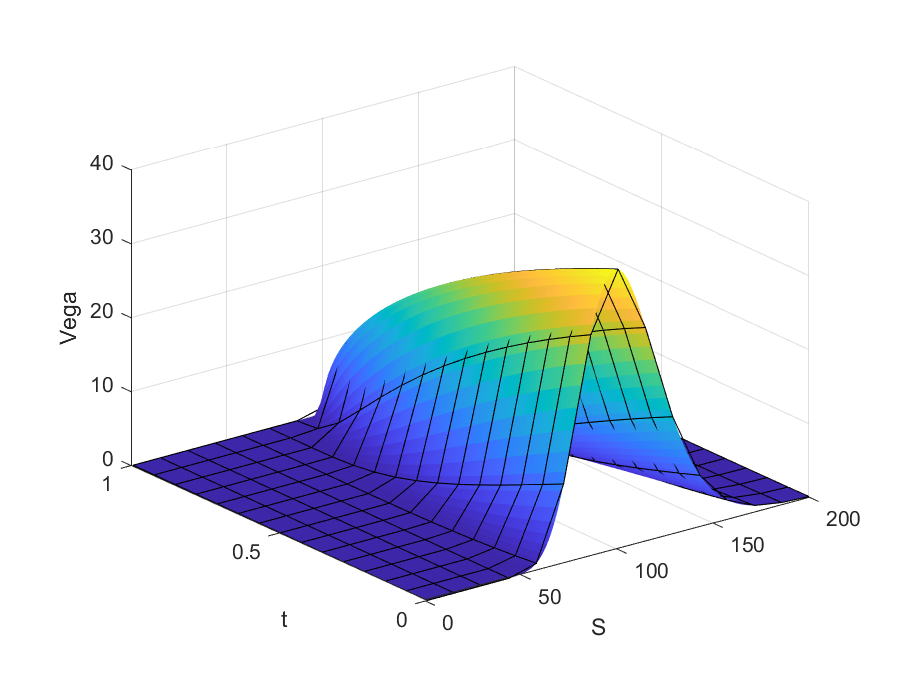
\includegraphics[width=\linewidth]{Imagenes/Parte1/6_Sols/Put/Put_Vega.eps}
        \caption{Vega}
    \end{subfigure}
    \begin{subfigure}[b]{0.35\linewidth}
        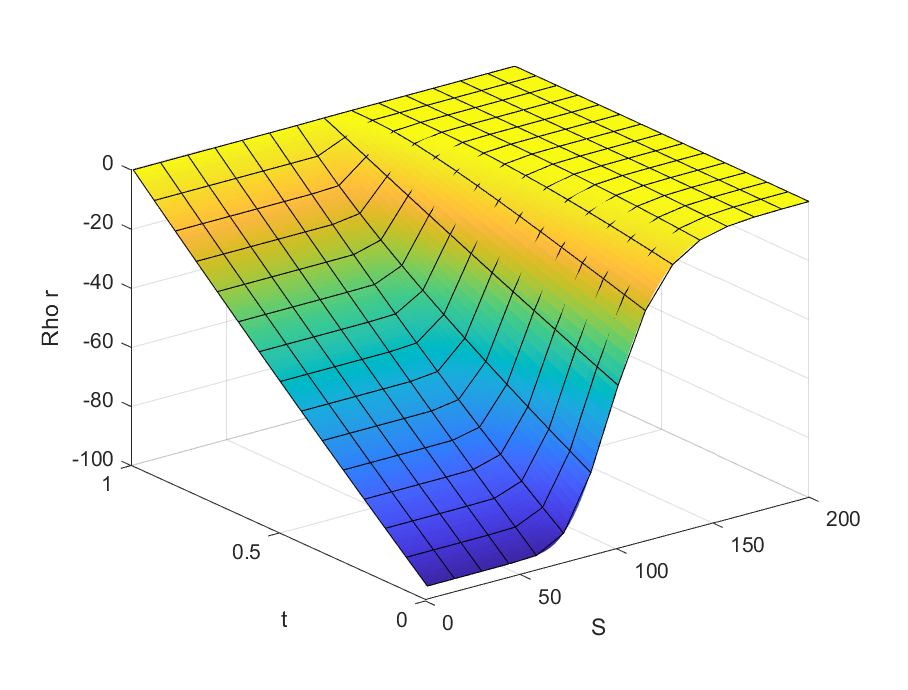
\includegraphics[width=\linewidth]{Imagenes/Parte1/6_Sols/Put/Put_Rho_r.eps}
        \caption{Rho (r)}
    \end{subfigure}
    \begin{subfigure}[b]{0.35\linewidth}
        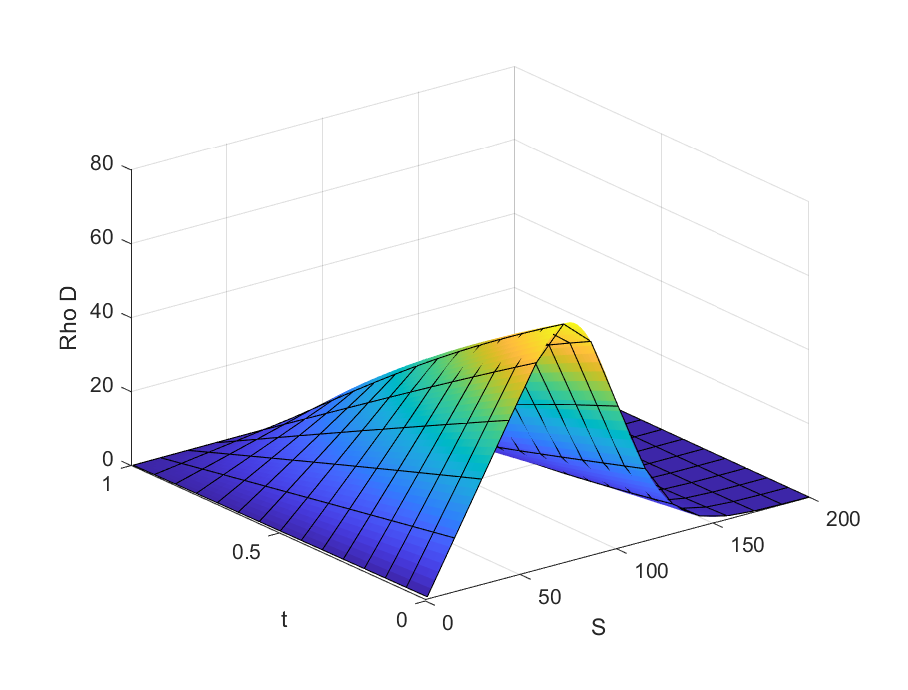
\includegraphics[width=\linewidth]{Imagenes/Parte1/6_Sols/Put/Put_Rho_D.eps}
        \caption{Rho (D)}
    \end{subfigure}
\end{figure}



\subsubsection{Binary Call option}
\begin{figure}[H]
    \centering
    \begin{subfigure}[b]{0.35\linewidth}
        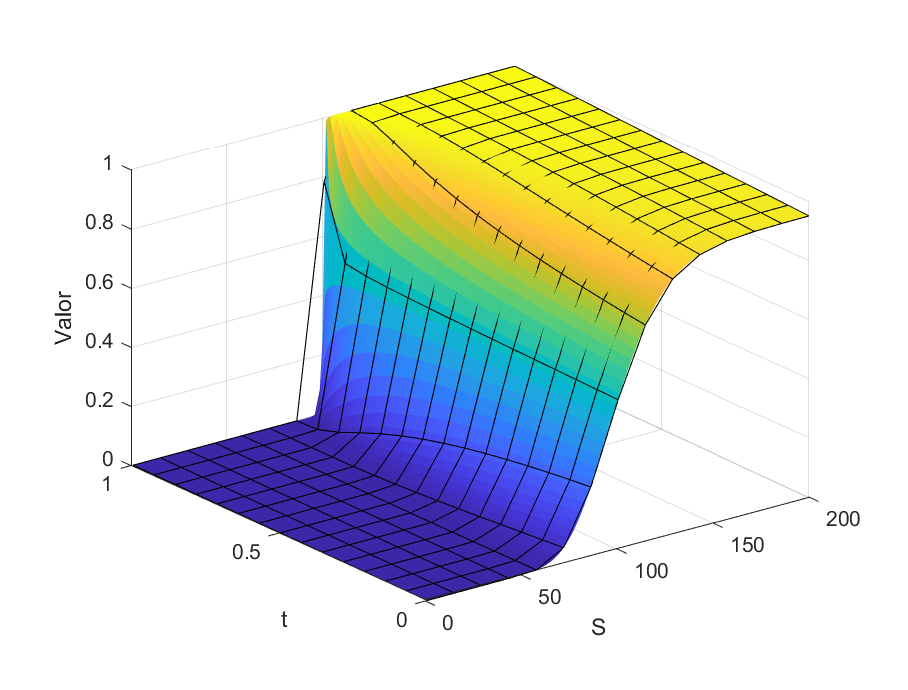
\includegraphics[width=\linewidth]{Imagenes/Parte1/6_Sols/Binary_Call/BinaryCall3D.eps}
        \caption{Solución}
    \end{subfigure}
    \begin{subfigure}[b]{0.35\linewidth}
        \includegraphics[width=\linewidth]{Imagenes/Parte1/6_Sols/Binary_Call/BinaryCallSFijo.eps}
        \caption{Solución con S fijo}
    \end{subfigure}
    \begin{subfigure}[b]{0.35\linewidth}
        \includegraphics[width=\linewidth]{Imagenes/Parte1/6_Sols/Binary_Call/BinaryCalltFIjo.eps}
        \caption{Solución con t fijo}
    \end{subfigure}
    \begin{subfigure}[b]{0.35\linewidth}
        \includegraphics[width=\linewidth]{Imagenes/Parte1/6_Sols/Binary_Call/Binary_Call_Delta.eps}
        \caption{Delta}
    \end{subfigure}
    \begin{subfigure}[b]{0.35\linewidth}
        \includegraphics[width=\linewidth]{Imagenes/Parte1/6_Sols/Binary_Call/Binary_Call_Gamma.eps}
        \caption{Gamma}
    \end{subfigure}
    \begin{subfigure}[b]{0.35\linewidth}
        \includegraphics[width=\linewidth]{Imagenes/Parte1/6_Sols/Binary_Call/Binary_Call_Theta.eps}
        \caption{Theta}
    \end{subfigure}
    \begin{subfigure}[b]{0.35\linewidth}
        \includegraphics[width=\linewidth]{Imagenes/Parte1/6_Sols/Binary_Call/Binary_Call_Speed.eps}
        \caption{Speed}
    \end{subfigure}
    \begin{subfigure}[b]{0.35\linewidth}
        \includegraphics[width=\linewidth]{Imagenes/Parte1/6_Sols/Binary_Call/Binary_Call_Vega.eps}
        \caption{Vega}
    \end{subfigure}
    \begin{subfigure}[b]{0.35\linewidth}
        \includegraphics[width=\linewidth]{Imagenes/Parte1/6_Sols/Binary_Call/Binary_Call_Rho_r.eps}
        \caption{Rho (r)}
    \end{subfigure}
    \begin{subfigure}[b]{0.35\linewidth}
        \includegraphics[width=\linewidth]{Imagenes/Parte1/6_Sols/Binary_Call/Binary_Call_Rho_D.eps}
        \caption{Rho (D)}
    \end{subfigure}
\end{figure}


\subsubsection{Binary Put option}
\begin{figure}[H]
    \centering
    \begin{subfigure}[b]{0.35\linewidth}
        \includegraphics[width=\linewidth]{Imagenes/Parte1/6_Sols/Binary_Put/BinaryPut3D.eps}
        \caption{Solución}
    \end{subfigure}
    \begin{subfigure}[b]{0.35\linewidth}
        \includegraphics[width=\linewidth]{Imagenes/Parte1/6_Sols/Binary_Put/BinaryPutSFijo.eps}
        \caption{Solución con S fijo}
    \end{subfigure}
    \begin{subfigure}[b]{0.35\linewidth}
        \includegraphics[width=\linewidth]{Imagenes/Parte1/6_Sols/Binary_Put/BinaryPuttFIjo.eps}
        \caption{Solución con t fijo}
    \end{subfigure}
    \begin{subfigure}[b]{0.35\linewidth}
        \includegraphics[width=\linewidth]{Imagenes/Parte1/6_Sols/Binary_Put/Binary_Put_Delta.eps}
        \caption{Delta}
    \end{subfigure}
    \begin{subfigure}[b]{0.35\linewidth}
        \includegraphics[width=\linewidth]{Imagenes/Parte1/6_Sols/Binary_Put/Binary_Put_Gamma.eps}
        \caption{Gamma}
    \end{subfigure}
    \begin{subfigure}[b]{0.35\linewidth}
        \includegraphics[width=\linewidth]{Imagenes/Parte1/6_Sols/Binary_Put/Binary_Put_Theta.eps}
        \caption{Theta}
    \end{subfigure}
    \begin{subfigure}[b]{0.35\linewidth}
        \includegraphics[width=\linewidth]{Imagenes/Parte1/6_Sols/Binary_Put/Binary_Put_Speed.eps}
        \caption{Speed}
    \end{subfigure}
    \begin{subfigure}[b]{0.35\linewidth}
        \includegraphics[width=\linewidth]{Imagenes/Parte1/6_Sols/Binary_Put/Binary_Put_Vega.eps}
        \caption{Vega}
    \end{subfigure}
    \begin{subfigure}[b]{0.35\linewidth}
        \includegraphics[width=\linewidth]{Imagenes/Parte1/6_Sols/Binary_Put/Binary_Put_Rho_r.eps}
        \caption{Rho (r)}
    \end{subfigure}
    \begin{subfigure}[b]{0.35\linewidth}
        \includegraphics[width=\linewidth]{Imagenes/Parte1/6_Sols/Binary_Put/Binary_Put_Rho_D.eps}
        \caption{Rho (D)}
    \end{subfigure}
\end{figure}





\subsection{Volatilidad implícita}\label{sec:vol_imp}
Valor de $\sigma$ que iguala precio teórico (Black-Scholes) al precio de mercado. Para su cálculo se utilizan métodos numéricos como Newton-Raphson usando vega.\\
No es consistente si se calcula para diferentes strikes y vencimientos, lo que genera distintas curvas de volatilidad implícita:
\begin{itemize}
    \item \textbf{Smile:} Volatilidad más alta para opciones ITM y OTM, mínima en ATM.\@
    \item \textbf{Skew:} Inclinación de la curva; típicamente negativa en mercados de acciones (mayor IV en puts OTM).
    \item \textbf{Frown:} Forma invertida del smile; menos común.
\end{itemize}
\begin{figure}[H]
    \centering
    \begin{subfigure}[b]{0.45\linewidth}
        \includegraphics[width=\linewidth]{Imagenes/Parte1/6_Sols/IV_vs_Strike.eps}
    \end{subfigure}
    \begin{subfigure}[b]{0.45\linewidth}
        \includegraphics[width=\linewidth]{Imagenes/Parte1/6_Sols/IV_vs_Delta.eps}
    \end{subfigure}
    \caption{Algunas curvas de volatilidad implícita}
\end{figure}






\subsection{Tipos de coberturas}
Según la independiencia con el modelo:
\begin{itemize}
    \item \textbf{Model-independent hedging:} Son pocos. No dependen de la dinámica del subyacente ni de la volatilidad. Por ejemplo la relación put-call parity.
    \item \textbf{Model-dependent hedging:} Son muchos más. Ejemplo más tipico es la cobertura usada en el análisis de Black-Scholes. Al valorar el derivado se necesita al menos la volatilidad.
\end{itemize}
Otros tipos de coberturas son:
\begin{itemize}
    \item \textbf{Delta hedging}: es la perfecta eliminación teórica del riesgo usando cobertura entre la opción y el subyacente. Es un ejemplo de cobertura \textbf{dinámica}: la cobertura se debe monitorizar y ajustar todo el rato, por lo que en la vida real va a dar lugar a pérdidas por los costes de transacción.
    \item \textbf{Gamma hedging}: usada para disminuir el tamaño de cada cobertura o para incrementar el tiempo entre coberturas (y así disminuir coste de transacción). Una cartera de este tipo es insensible a cambios del subyacente mientras sean movimientos pequeños. 
    \item \textbf{Vega hedging}: usada para eliminar el riesgo de volatilidad. En realidad esto en ocasiones da lugar a inconsistencias y no se debe usar una volatilidad constante.
    \item \textbf{Static hedging}: usada para reducir el riesgo de opciones exóticas mediante contratos más líquidos que se mantienen hasta el vencimiento, eliminando la necesidad de ajustes dinámicos.
    \item \textbf{Margin hedging}: usada para equilibrar las llamadas de margen (depósitos obligatorios) en una parte del portafolio con los reembolsos de otras partes, evitando así grandes llamadas de margen que puedan ser difíciles de cumplir.
    \item \textbf{Crash (Platinum) hedging}: diseñada para minimizar el peor resultado posible en mercados extremos (p.e.\ caídas), donde los movimientos son tan grandes que no se puede seguir el ritmo con las coberturas, y además las correlaciones normales se vuelven irrelevantes. Incluye dos tipos: cobertura del valor nominal del portafolio y cobertura de llamadas de margen.
\end{itemize}







  \newpage
  
\section{Generalizaciones sencillas del modelo}

\subsection{Dividendos discretos}
Para evitar arbitraje, el precio de una acción con dividendo $D_i$ en el instante $t_i$ debe debe cumplir la condición de salto:
\[
    S(t_i^+) = S(t_i^-) - D_i
\]
luego la opción que tenga esa acción como suyacente debe cumplir que
\[
    V(S(t_i^-), t_i^-) = V(S(t_i^+), t_i^+) \Rightarrow \boxed{V(S, t_i^-) = V(S - D_i, t_i^+)}
\]\label{eq:divs_discretos}
El valor de la opción no pega un salto en el instante $t_i$ y es continua.




\subsection{Préstamo de acciones}
Cuando se habla de ir \textit{short} en una acción, muchas veces no se tiene por lo que se pide prestada. Pero este préstamo tiene un coste de interés $R$ sobre el valor de la acción. Usando el mismo argumento que para el modelo básico de Black-Scholes:
\begin{align*}
    &\left\{ 
        \begin{array}{rcl} 
            dS &= \mu Sdt + \sigma S d\mathnormal{X} &\\ 
            \Pi &= V(S,t) - \Delta S &\Rightarrow d\Pi = dV- \Delta dS
        \end{array} 
    \right\} \Rightarrow \\
    \Rightarrow &d\Pi = \frac{\partial V}{\partial t}dt + \frac{\partial V}{\partial S}dS + \frac{\sigma^2S^2}{2} \frac{\partial^2 V}{\partial S^2}dt - \Delta dS
\end{align*}
Pero como ahora se tiene que pagar un interés por el préstamo de la acción:
\[
    d\Pi = \frac{\partial V}{\partial t}dt + \frac{\partial V}{\partial S}dS + \frac{\sigma^2S^2}{2} \frac{\partial^2 V}{\partial S^2}dt - \Delta dS - R\max(\Delta, 0)Sdt
\]
que, haciendo un \textbf{delta hedging} $\Delta = \frac{\partial V}{\partial S}$ se obtiene que, sin arbitraje:
\[
d\Pi = \left( \frac{\partial V}{\partial t} + \frac{\sigma^2S^2}{2} \frac{\partial^2 V}{\partial S^2} -RS\max\left(\frac{\partial V}{\partial S}, 0\right) \right)dt
\]
igualando a que $d\Pi = r\Pi dt$ se obtiene que
\[
\boxed{\frac{\partial V}{\partial t} + \frac{\sigma^2S^2}{2} \frac{\partial^2 V}{\partial S^2} + rS \frac{\partial V}{\partial S} -rV -RS\max\left(\frac{\partial V}{\partial S}, 0\right) = 0}
\]


\subsection{Parámetros dependientes del tiempo}
Para el caso de una opción europea, resolver el problema con parametros $r(t), D(t), \sigma(t)$ es lo mismo que reolverlo con los parámetros constantes
\[
    \boxed{
        \begin{aligned}
            r_c &= \frac{1}{T-t} \int_t^T r(\tau) d\tau \\
            D_c &= \frac{1}{T-t} \int_t^T D(\tau) d\tau \\
            \sigma_c^2 &= \frac{1}{T-t} \int_t^T \sigma^2(\tau) d\tau
        \end{aligned}
    }
\]
Para el caso de opciones americanas o exóticas se deben estudiar las condiciones de frontera.







\subsection{Power options y log contracts}
Se puede encontrar más información en el apéndice~\ref{ApexGenerals}.










  \newpage
  \section{Modelización la volatilidad}
Tipos de volatilidad:
\begin{itemize}
    \item \textbf{Actual volatility}: Es la medida de la cantidad de aleatoriedad en el retorno de un activo en un instante dado, variando de momento a momento sin asociarse a una escala temporal.
    \item \textbf{Historical or realized volatility}: Es una medida de la aleatoriedad en un periodo pasado específico, calculada con métodos matemáticos y utilizada como estimación para la volatilidad futura.
    \item \textbf{Implied volatility}: Es la volatilidad que, al ser introducida en el modelo de Black-Scholes, iguala el precio de mercado de la opción, reflejando la expectativa del mercado sobre la volatilidad futura. Se ha introducido en la sección~\ref{sec:vol_imp}.
    \item \textbf{Forward volatility}: Es la volatilidad asociada a un periodo de tiempo futuro o a un instante futuro, ya sea actual o implícita.
\end{itemize}



\subsection{Volatilidad por media estadística}

\subsubsection{Volatilidad constante}
Para el caso de volatilidad constante o variaciones lentas, entonces se puede considerar:
\[
\boxed{\sigma^2 = \frac{1}{N} \sum_{i=1}^{N} R_i^2}
\]
donde 
\[
R_i = \frac{S_i - S_{i-1}}{S_{i-1}}
\]
representa el retorno del día $i$. Este método tiene limitaciones, como el efecto espurio que hace que por picos instantáneos muy altos o muy bajos, la volatilidad se mantendrá muy alta durante unos días.


\subsubsection{Volatilidad con regresión a la media}
Considerando una volatilidad dependiente del tiempo y para modelar que la volatilidad tiende a una media a largo plazo $\overline{\sigma}$, se usa el modelo \textbf{ARCH (Autoregressive Conditional Heteroscedasticity)} asigna un peso a cada estimación de volatilidad a largo plazo y a la estimación actual basada en los últimos $n$ retornos:
\[
\boxed{\sigma_n^2 = \alpha \overline{\sigma}^2 + (1 - \alpha) \frac{1}{n} \sum_{i=1}^{n} R_i^2}
\]
Donde $\alpha$ es el parámetro que controla la importancia relativa entre la volatilidad a largo plazo y la volatilidad basada en los retornos recientes.



\subsubsection{Volatilidad con media móvil exponencialmente ponderada (EWMA)}
Se utiliza el modelo:
\[
\sigma_n^2 = (1 - \lambda) \sum_{i=1}^{\infty} \lambda^{i-1} R_{n-i+1}^2
\]
donde $\lambda$ es un parámetro entre 0 y 1 que controla el peso de los retornos pasados. Este modelo asigna mayor peso a los retornos más recientes. La expresión puede simplificarse como:
\[
\boxed{\sigma_n^2 = \lambda \sigma_{n-1}^2 + (1 - \lambda) R_n^2}
\]
Esto utiliza el retorno más reciente y la estimación previa de la volatilidad, siendo conocido como la medida de volatilidad de RiskMetrics.


\subsubsection{Modelo GARCH}
El modelo GARCH (Generalized Autoregressive Conditional Heteroscedasticity) combina la volatilidad a largo plazo, la volatilidad previa y los retornos recientes para estimar la volatilidad actual:
\[
\boxed{\sigma_n^2 = \alpha \overline{\sigma}^2 + (1 - \alpha) \left( \lambda \sigma_{n-1}^2 + (1 - \lambda) R_n^2 \right)}
\]
Este modelo es útil para capturar la dinámica de la volatilidad en el tiempo, considerando tanto la persistencia como la regresión hacia una media a largo plazo.

\subsubsection{Volatilidad futura esperada}
Estando a día $n$ se quiere estimar la volatilidad en $k$ días, i.e.\ en el día $n+k$. Dos maneras de hacerlo son:
\begin{itemize}
    \item Modelo \textbf{EWMA}:
    \begin{align*}
        \sigma_{n+k}^2 &= \lambda \sigma_{n+k-1}^2 + (1 - \lambda) R_{n+k}^2 \Rightarrow \\
        \Rightarrow \mathbb{E}[\sigma_{n+k}^2] &= \lambda \mathbb{E}[\sigma_{n+k-1}^2] + (1 - \lambda) \mathbb{E}[R_{n+k}^2] \Rightarrow \\
        \Rightarrow \mathbb{E}[\sigma_{n+k}^2] &= \lambda \mathbb{E}[\sigma_{n+k-1}^2] + (1 - \lambda) \mathbb{E}[\sigma_{n+k}^2]
    \end{align*}
    luego
    \[
    \boxed{\mathbb{E}[\sigma_{n+k}^2] = \mathbb{E}[\sigma_{n+k-1}^2]}
    \]
    Esto implica que la volatilidad futura esperada es igual a la estimación de volatilidad del día anterior.
    \item Modelo \textbf{GARCH}:
    \begin{align*}
        \sigma_{n+k}^2 &= \alpha \overline{\sigma}^2 + (1 - \alpha) \left( \lambda \sigma_{n+k-1}^2 + (1 - \lambda) R_{n+k}^2 \right) \Rightarrow \\
        \Rightarrow \mathbb{E}[\sigma_{n+k}^2] &= \alpha \overline{\sigma}^2 + (1 - \alpha) \left( \lambda \mathbb{E}[\sigma_{n+k-1}^2] + (1 - \lambda) \mathbb{E}[R_{n+k}^2] \right) \Rightarrow\\
        \Rightarrow \mathbb{E}[\sigma_{n+k}^2] &= \frac{\alpha \overline{\sigma}^2}{1 - (1 - \alpha)(1 - \lambda)} + \frac{\lambda (1 - \alpha)}{1 - (1 - \alpha)(1 - \lambda)} \mathbb{E}[\sigma_{n+k-1}^2]
    \end{align*}
    Mirando más hacia el futuro:
    \[
    \boxed{\mathbb{E}[\sigma_{n+k}^2] = \overline{\sigma}^2 + \left( \mathbb{E}[\sigma_{n}^2] - \overline{\sigma}^2 \right) (1 - \nu)^k} \text{ , } \qquad \nu = \frac{\alpha}{1 - (1 - \alpha)(1 - \lambda)}
    \]
\end{itemize}


\begin{figure}[H]
    \centering
    \begin{subfigure}[b]{0.45\linewidth}
        \includegraphics[width=\linewidth]{Imagenes/Parte1/7_Volatilidad/Volatilidad.eps}
    \end{subfigure}
    \begin{subfigure}[b]{0.5\linewidth}
        \includegraphics[width=\linewidth]{Imagenes/Parte1/7_Volatilidad/Volatilidad_Prediccion.eps}
    \end{subfigure}
    \begin{subfigure}[b]{0.45\linewidth}
        \includegraphics[width=\linewidth]{Imagenes/Parte1/7_Volatilidad/Accion.eps}
    \end{subfigure}
    \caption{Comparación de estimadores de volatilidad}
\end{figure}



\subsubsection{Estimación de volatilidad basada en rangos de tiempo}
Usar demasiados datos puede capturar variaciones temporales del parámetro, mientras que usar pocos datos puede generar errores de muestreo. En primer lugar, sabiendo que \textit{Varianza\_anual = Varianza\_diaria $\times$ Número\_días\_trading}, entonces la volatilidad anualizada sería:
\[
\boxed{\sigma_{anual} = \sigma_{diaria} \times \sqrt{\textit{Número\_días\_trading}}}
\]
Algunas maneras de estimar la volatilidad diaria según los rangos de tiempo son:
\begin{itemize}
    \item \textbf{Medición tradicional close-to-close}: Sea $C_i$ el precio de cierre del día $i$, entonces:
    \begin{itemize}
        \item \textbf{Drift pequeño}:
        \[
        \boxed{\sigma^2_{cc} = \frac{1}{n} \sum_{i=1}^{n} \left( \log \left( \frac{C_i}{C_{i-1}} \right) \right)^2}
        \]
        \item \textbf{Drift genérico}:
        \[
        \boxed{\sigma^2_{acc} = \frac{1}{n-1} \sum_{i=1}^{n} \left( \left( \log \left( \frac{C_i}{C_{i-1}} \right) \right)^2 - \frac{\left( \log \left( \frac{C_n}{C_0} \right) \right)^2}{n(n-1)} \right)}
        \]
    \end{itemize}
    \item \textbf{Medición basada en rangos extremos (Parkinson, 1980)}: Utiliza los valores extremos del día, los máximos $H_i$ y los mínimos $L_i$. Es 5 veces más efectiva que la medición close-to-close:
    \[
    \boxed{\sigma_p^2 = \frac{1}{4n \log(2)} \sum_{i=1}^{n} \left( \log \left( \frac{H_i}{L_i} \right) \right)^2}
    \]

    \item \textbf{Medición basada en rangos extremos y apertura (Garman \& Klass, 1980)}: Utiliza los valores extremos del día y el precio de apertura $O_i$. Es 7.4 veces más efectiva que la medición close-to-close:
    \[
    \boxed{\sigma_{gk}^2 = \frac{1}{n} \sum_{i=1}^{n} \left( 0.511 \left( \log \left( \frac{H_i}{L_i} \right) \right)^2 - 0.019 \log \left( \frac{C_i}{O_i} \right) - 2 \log \left( \frac{H_i}{O_i} \right) \log \left( \frac{L_i}{O_i} \right) \right)}
    \]

    \item \textbf{Medición basada en rangos extremos y cierre (Rogers \& Satchell, 1991)}: Es independiente del drift, no como Parkinson y Garman \& Klass:
    \[
    \boxed{\sigma_{rs}^2 = \frac{1}{n} \sum_{i=1}^{n} \left( \log \left( \frac{H_i}{C_i} \right) \log \left( \frac{H_i}{O_i} \right) + \log \left( \frac{L_i}{C_i} \right) \log \left( \frac{L_i}{O_i} \right) \right)}
    \]
\end{itemize}





\subsection{Estimar parámetros: maximum likelihood estimation (MLE)}
Llegas a una ciudad y coges el taxi número 20922, ¿cuantos taxis hay en la ciudad? El concepto del MLE consiste en elegir los parámetros de manera que se maximice la probabilidad de que ocurra el evento observado. En este caso, la probabilidad de subirse en un taxi en específico es de $1/N$ y el $N$ que maximiza la probabilidad de subirse en el taxi 20922 es $N=20922$ $(100\%)$.

La lógica es la siguiente: se tiene un modelo (p.e.\ una normal de media 0 y desviación a estimar) con 3 (o los que sean) parámetros (p.e.\ desviación). Obtengo varios datos, calculo su probabilidad de ocurrir para cada uno de los modelos, hago una probabilidad conjunta de todos los datos y se elige el modelo que maximice esa probabilidad conjunta.

Matemáticamente, el proceso es el siguiente, sabiendo que para una distribución normal con media cero y desviación estándar $\sigma$, la probabilidad de obtener un valor $\phi_i$ es:
\[
\frac{1}{\sqrt{2\pi}\sigma} e^{-\frac{\phi_i^2}{2\sigma^2}}
\]
Luego la probabilidad conjunta de obtener $N$ valores $\phi_1, \phi_2, \dots, \phi_N$ es:
\[
\prod_{i=1}^N \frac{1}{\sqrt{2\pi}\sigma} e^{-\frac{\phi_i^2}{2\sigma^2}}
\]
Para maximizar esta probabilidad conjunta, se deriva con respecto a $\sigma$:
\begin{align*}
    &\frac{\partial}{\partial \sigma} \left( \prod_{i=1}^N \frac{1}{\sqrt{2\pi}\sigma} \exp\left(-\frac{\phi_i^2}{2\sigma^2}\right) \right) = 0 \Rightarrow \\
    \Rightarrow &\frac{\partial}{\partial \sigma} \left( \left( \frac{1}{\sqrt{2\pi}\sigma} \right)^N \exp\left(-\frac{1}{2\sigma^2} \sum_{i=1}^N \phi_i^2\right) \right) = 0 \Rightarrow \\
    \Rightarrow &\frac{\partial}{\partial \sigma} \left( \ln\left(\left( \frac{1}{\sqrt{2\pi}\sigma} \right)^N \exp\left(-\frac{1}{2\sigma^2} \sum_{i=1}^N \phi_i^2\right)\right) \right) = 0 \Rightarrow \\
    \Rightarrow &\frac{\partial}{\partial \sigma} \left( N\ln\left(\frac{1}{\sqrt{2\pi}\sigma}\right) - \frac{1}{2\sigma^2} \sum_{i=1}^N \phi_i^2 \right) = 0 \Rightarrow \\
    \Rightarrow &\frac{\partial}{\partial \sigma} \left( -N\ln\left(\sqrt{2\pi}\right) -N\ln\left(\sigma\right) - \frac{1}{2\sigma^2} \sum_{i=1}^N \phi_i^2 \right) = 0 \Rightarrow \\
    \Rightarrow &-\frac{N}{\sigma} + \frac{1}{\sigma^3} \sum_{i=1}^N \phi_i^2 = 0 \Rightarrow \\
    \Rightarrow &\sigma^2 = \frac{1}{N} \sum_{i=1}^N \phi_i^2
\end{align*}







\subsection{Volatilidad dependiente del tiempo en modelos sencillos}\label{sec:vol_dep_tiempo}
Cuando se tiene una volatilidad dependiente del tiempo pero el modelo utiliza una volatilidad constante, se puede considerar una volatilidad constante promedio de forma similar a lo que se hace en las opciones asiáticas:
\begin{equation*}
    \boxed{\overline{\sigma}^2 = \frac{1}{T} \int_0^T \sigma(t)^2 dt}
\end{equation*}





  \newpage
  \section{Cobertura: volatilidad implicita vs real}
Esta sección se centra en el caso en el que la volatilidad implícita es diferencte a la volatilidad que se ha calculado a partir de los datos históricos.
Si se compra un ATM strandle, el beneficio esperado es aproximadamente de
\[
\sqrt{\frac{2(T-t)}{\pi}}\, (\sigma - \tilde{\sigma})\, S.
\]
con una desviación típica de
\[
\sqrt{1 - \frac{2}{\pi}}\, \sigma S \sqrt{T-t}.
\]
donde $\sigma$ es la volatilidad real y $\tilde{\sigma}$ es la volatilidad implícita. La desviación depende de la volatilidad y tiene la misma magnitud que la media, por lo que el riesgo es muy alto, por lo que se debe seguir alguna estrategia para minimizar riesgos.

\begin{notation}
    Se define la $a$ superíndice para la volatilidad real y la $i$ como superíndice para la volatilidad implícita. Por ejemplo, $V^a$ es la delta usando la volatilidad real en la fórmula y $V^i$ es la delta usando la volatilidad implícita en la fórmula.
\end{notation}

Según sobre que volatilidad se decida hacer la cobertura, se obtiene distintos resultados:
\begin{itemize}
    \item \textbf{Cobertura sobre la volatilida real}: Sea el modelo
    \[
        dS = \mu S dt + \sigma S dX.
    \]
    se construye una cartera comprando la opción por $V^i$ y cubriendo con $\Delta^a$ del subyacente, lo que da lugar a un efectivo de $-V^i + \Delta^a S$. Es decir las cartera es:
    \begin{table}[H]
        \centering
        \begin{tabular}{l|c}
            \textbf{Componente} & \textbf{Valor} \\
            \hline
            Opción & $V^i$ \\
            Acción & $-\Delta^a S$ \\
            Efectivo & $-V^i + \Delta^a S$ \\
        \end{tabular}
    \end{table}
    \[
        \Pi = V^i-\Delta^a S-V^i + \Delta^a S
    \]
    Se supone además unos dividendos continuos de $D$ y una tasa de interés $r$. Entonces, la variación de la cartera es
    \[
        d\Pi = dV^i - \Delta^a dS - r(V^i - \Delta^a S)dt - \Delta^a D S dt
    \]
    Asumiendo que la opción está correctamente valorada en $V^a$, se tiene que
    \begin{align*}
        &dV^a - \Delta^a dS - r(V^a - \Delta^a S)dt - \Delta^a D S dt = 0 \Rightarrow \\
        \Rightarrow  &-\Delta^a dS - \Delta^a D S dt = -dV^a + r(V^a - \Delta^a S)dt
    \end{align*}
    por lo que sustituyendo en la variación de la cartera se obtiene
    \begin{align*}
        d\Pi &= dV^i - r(V^i - \Delta^a S)dt -dV^a - r(V^a - \Delta^a S)dt \\
        &= dV^i - dV^a - r(V^i - V^a)dt
    \end{align*}
    Se sabe que
    \begin{align*}
        &\frac{d}{dt} \left( e^{-rt}(V^i - V^a)\right) = -r e^{-rt}(V^i - V^a) + e^{-rt}\left(\frac{d}{dt}V^i - \frac{d}{dt}V^a\right) \Rightarrow \\
        \Rightarrow & d(e^{-rt}(V^i - V^a)) = e^{-rt}\left( -r(V^i - V^a)dt + dV^i - dV^a \right) \Rightarrow \\
        \Rightarrow & e^{rt}d(e^{-rt}(V^i - V^a)) = -r(V^i - V^a)dt + dV^i - dV^a \Rightarrow \\
    \end{align*}
    que sustituyendo en la variación de la cartera se obtiene
    \begin{align*}
        d\Pi &= dV^i - dV^a + e^{rt}d(e^{-rt}(V^i - V^a)) + dV^a - dV^i \\
        &= e^{rt}d(e^{-rt}(V^i - V^a))
    \end{align*}
    que actualizada actualizada a tiempo $t_0$ es
    \begin{align*}
        d\Pi &= e^{-r(t-t_0)}e^{rt}d(e^{-rt}(V^i - V^a)) \\
        &= e^{rt_0}d(e^{-rt}(V^i - V^a))
    \end{align*}
    La ganacia total desde $t_0$ hasta el vencimiento es
    \begin{align*}
        \int_{t_0}^T d\Pi &= \int_{t_0}^T e^{-rt_0}d(e^{rt}(V^i - V^a))\\
        &= e^{-rt_0}\left[ e^{rT}(V^i(T) - V^a(T)) - e^{rt_0}(V^i(t_0) - V^a(t_0))\right] = \\
        &= e^{-rt_0}\left[ - e^{rt_0}(V^i(t_0) - V^a(t_0))\right]
    \end{align*}
    Por lo tanto, el beneficio total garantizado al vencimiento es
    \[
        \boxed{V^a(t_0) - V^i(t_0) }
    \]
    Se debe de tener en cuenta que el beneficio final está garantizado, pero los beneficios en el camino son aleatorios.

    Se puede desmostrar que la variación de la cartera tambien se puede escribir como
    \[
        \frac{1}{2}(\sigma^2 - \tilde{\sigma}^2)S^2 \Gamma^i dt + (\Delta^i - \Delta^a)\left((\mu - r + D)S dt + \sigma S dX\right)
    \]
    
    \item \textbf{Cobertura sobre la volatilidad implícita}:Se usa igualmente el modelo
    \[
        dS = \mu S dt + \sigma S dX
    \]
    y se construye la cartera
    \[
        \Pi = V^i-\Delta^i S-V^i + \Delta^i S
    \]
    Sabiendo que hay un dividendos continuos, entonces su variación es
    \begin{align*}
        d\Pi &= dV^i - \Delta^i dS - r(V^i - \Delta^i S)dt - \Delta^i D S dt \\
        &= \Theta^i dt + \frac{1}{2} \sigma^2 S^2 \Gamma^i dt - r(V^i - \Delta^i S)dt - \Delta^i D S dt \\
        &= \frac{1}{2}(\sigma^2 - \tilde{\sigma}^2)S^2 \Gamma^i dt
    \end{align*}
    que actualizada a tiempo $t_0$ es
    \[ 
        d\Pi = e^{r(t-t_0)}\frac{1}{2}(\sigma^2 - \tilde{\sigma}^2)S^2 \Gamma^i dt
    \]
    \begin{figure}[H]
        \centering
        \includegraphics[width=0.65\linewidth]{Imagenes/Parte1/10_Cobertura/Cobertura_Volat_Imp.pdf}
        \caption{Beneficios de cobertura sobre la volatilidad implícita}
    \end{figure}
    por lo que en tiempo final hay un beneficio debe ser
    \[
        \boxed{\int_{t_0}^T d\Pi = \frac{1}{2}(\sigma^2 - \tilde{\sigma}^2) \int_{t_0}^T e^{r(t-t_0)}S^2 \Gamma^i dt}
    \]
    que es siempre positivo si la volatilidad real es mayor que la implícita. Se puede calcular la media y varianza de este beneficio. Para mas información, ver el apéndice~\ref{ApexCobVolImp}.

    Por lo tanto, el beneficio solo depende de gamma, por lo que las opciones put call tienen el mismo beneficio esperado. Si se construyen carteras con opciones con distintos strikes, se obtiene un beneficio de
    \[
        \frac{1}{2}\sum_k(\sigma^2 - \tilde{\sigma_k}^2) \int_{t_0}^{T_k} e^{r(t-t_0)}S^2 \Gamma^i_k dt
    \]
    cuya media y varianza se pueden calcular.
    \item \textbf{Cobertura cuando la volatilidad implícita es aleatoria}: Sean los modelos
    \begin{align*}
        dS &= \mu S dt + \sigma S dX_1 \\
        d\tilde{\sigma} &= a dt + b dX_2
    \end{align*}
    y la correlación $\rho$ entre $dX_1$ y $dX_2$.
    \begin{itemize}
        \item \textbf{Cobertura sobre la volatilidad real}: Usando los mismo argumentos que antes, se llega a que el beneficio final está asegurado. Por otro lado, la variación de la cartera está
        \begin{align*}
            d\Pi =& \frac{1}{2}(\sigma^2 - \tilde{\sigma}^2)S^2 \Gamma^i\, dt + (\Delta^i - \Delta^a)\left( (\mu - r + D)S\, dt + \sigma S\, dX_1 \right) + \\
            &+\frac{\partial V^i}{\partial \tilde{\sigma}}\, d\tilde{\sigma} + \frac{1}{2} b^2 \frac{\partial^2 V^i}{\partial \tilde{\sigma}^2}\, dt + \rho \sigma b S \frac{\partial^2 V^i}{\partial S \partial \tilde{\sigma}}\, dt.
        \end{align*}
        \item \textbf{Cobertura sobre la volatilidad implícita}: Usando los mismos argumentos que antes se llega a que la variación de la cartera está
        \begin{align*}
        d\Pi =&dV^i - \Delta dS - r(V^i - \Delta S)dt - \Delta D S dt\\
        =& \Theta^i dt + \Delta^i dS + \frac{1}{2} \sigma^2 S^2 \Gamma^i dt + \frac{\partial V^i}{\partial \tilde{\sigma}} d\tilde{\sigma} + \frac{1}{2} b^2 \frac{\partial^2 V^i}{\partial \tilde{\sigma}^2} dt \\
        &+ \rho \sigma b S \frac{\partial^2 V^i}{\partial S \partial \tilde{\sigma}} dt - \Delta dS - r(V^i - \Delta S)dt - \Delta D S dt.
        \end{align*}
        se puede obtener su esperanza y varianza.
    \end{itemize}
\end{itemize}

\subsection{Comportamiento de la volatilidad implícita}
Existen varios ``modelos'' de cómo se comporta la volatilidad implícita:
\begin{itemize}
    \item \textbf{Sticky Strike}: es constante para cada opción (i.e.\ para cada strike y vencimiento). Es común en los mercados de renta variable. Si la volatilidad implícita difiere de la volatilidad real se pueden obtener beneficios como se ha explicado.
    \item \textbf{Sticky Delta}: depende de su moneyness ($\xi = S/E$). Es común en mercados como el FX, donde se cotizan precios y volatilidades para opciones con deltas específicas. Se modela como $\tilde{\sigma} = g(\xi, t)$ por lo que:
    \[
        d\tilde{\sigma} = \left( \frac{\partial g}{\partial t} + \mu \frac{S}{E} \frac{\partial g}{\partial \xi} + \frac{1}{2} \sigma^2 \frac{S^2}{E^2} \frac{\partial^2 g}{\partial \xi^2} \right) dt + \sigma \frac{S}{E} \frac{\partial g}{\partial \xi} dX_1,
    \]
    La variación de la volatilidad implícita está perfectamente correlacionada con el subyacente, permitiendo una cobertura perfecta en términos de mark-to-market.

    Hay una variantes donde la volatilidad implícita depende de la volatilidad ATM y de una función del moneyness, por ejemplo:
    \[
        \tilde{\sigma} = \sigma_{ATM} \, g\left( \frac{\log(S/E)}{\sqrt{T-t}} \right).
    \]
\end{itemize}






  \newpage
  
\section{Opciones americanas}

Aquellas que pueden ejercerse en cualquier momento antes de su vencimiento. Sea $\Phi(S)$ el payoff de la opción, entonces se cumple que:
\[
\boxed{V \geq \Phi(S)}
\]\label{eq:cond_op_americana}
Si no fuese el caso, entonces $V < \Phi(S) \Rightarrow \Phi(S) - V > 0$, por lo que se podría comprar una opción y ejercer al momento obteniendo un beneficio sin riesgo, por lo que habría arbitraje.

En general, el punto óptimo de ejercicio es aquel que hace que la pendiente de la opción sea la misma que la pendiente del \textit{payoff}.

Sea la cartera
\[
\Pi = V - \Delta S
\]
entonces la diferencia entre el cambio de valor de la cartera y su crecimiento por el interés es:
\[
d\Pi - r\Pi dt = \left( \frac{\partial V}{\partial t} + \frac{1}{2} \sigma^2 S^2 \frac{\partial^2 V}{\partial S^2} - r(V - \Delta S) \right) dt + \left( \frac{\partial V}{\partial S} - \Delta \right) dS
\]
y eligiendo $\Delta = \frac{\partial V}{\partial S}$, se obtiene:
\[
d\Pi - r\Pi dt = \left( \frac{\partial V}{\partial t} + \frac{1}{2} \sigma^2 S^2 \frac{\partial^2 V}{\partial S^2} - rV \right) dt
\]
Para evitar arbitraje solo se debe asegurar que esta resta sea no positiva, de manera que la cartera no gane mas que el interés:
\[
\boxed{\frac{\partial V}{\partial t} + \frac{1}{2} \sigma^2 S^2 \frac{\partial^2 V}{\partial S^2} - rV \leq 0}
\]
El caso $\cdots < 0$ no produce arbitraje porque al vender una opción y meterlo en el banco (para que crezca a ritmo $r$), se corre el riesgo de que el comprador ejerza en cualquier momento.


\subsection{Dividendos discretos}
Como se ha visto en la ecuacion~\eqref{eq:divs_discretos}, si hay dividendo discreto se cumple que $V(S, t_i^-) = V(S - D_i, t_i^+)$, por lo que para evitar que el valor de la opción caiga por debajo del valor de ejercicio inmediato se impone
\[
\boxed{V(S, t_d^-) = \max\left(V(S - D, t_d^+), \Phi(S)\right)}
\]
garantizando que el valor de la opción nunca sea menor que el payoff si se ejerciera justo antes del dividendo evitando así arbitraje.





\subsection{Opciones one-touch}
Es una versión americana de la opción binaria  europea. Se paga una cantidad fija si el subyacente alcanza una cierta barrera antes de vencimiento. El pago realiza tan pronto como se alcanza la barrera, sin esperar al vencimiento.
\begin{itemize}
    \item \textbf{One-touch call:} paga si el subyacente $S$ alcanza un nivel superior $S_u$.
    \[
        \boxed{V(S, t) = \left( \frac{S_u}{S} \right)^{2r/\sigma^2} N(d_6) + \frac{S}{S_u} N(d_1)}
    \]
    donde
    \[
        \boxed{d_6 = \frac{\log(S/S_u) - (r + \frac{1}{2}\sigma^2)(T-t)}{\sigma\sqrt{T-t}}}
    \]
    y $d_1$ es el mismo que en Black-Scholes~\eqref{eq:d_sol_BS}.
    \begin{figure}[H]
        \centering
        \begin{subfigure}[b]{0.35\linewidth}
            \includegraphics[width=\linewidth]{Imagenes/Parte1/9_Americanas/One_Touch_Call.pdf}
            \caption{Solución de una opción one-touch call}
        \end{subfigure}
        \begin{subfigure}[b]{0.35\linewidth}
            \includegraphics[width=\linewidth]{Imagenes/Parte1/9_Americanas/Delta_One_Touch_Call.pdf}
            \caption{Delta de una opción one-touch call}
        \end{subfigure}
    \end{figure}
    \item \textbf{One-touch put:} paga si $S$ cae hasta un nivel inferior $S_l$.
    \[
        \boxed{V(S, t) = \left( \frac{S_l}{S} \right)^{2r/\sigma^2} N(-d_6) + \frac{S}{S_l} N(-d_1)}
    \]
    con
    \[
        \boxed{d_6 = \frac{\log(S/S_l) - (r + \frac{1}{2}\sigma^2)(T-t)}{\sigma\sqrt{T-t}}}
    \]
    y $d_1$ es el mismo que en Black-Scholes~\eqref{eq:d_sol_BS}.
    \item \textbf{Double one-touch:} paga si $S$ alcanza cualquiera de dos barreras (superior $S_u$ o inferior $S_l$) antes del vencimiento. El valor se puede calcular mediante series de Fourier y no es simplemente la suma de una call y una put one-touch.
\end{itemize}




\subsection{Otros tipos de opciones americanas}
\begin{itemize}
    \item \textbf{Opciones israelíes}: opciones americanas en las que el escritor puede cancelar la opción más temprano pagando una penalización.
    \item \textbf{Opciones Bermuda}: opciones americanas que solo pueden ejercerse en fechas específicas, no en cualquier momento. Lo único que cambia con respecto a las americanas es que la condición~\eqref{eq:cond_op_americana} se aplica solo en los momentos de ejercicio permitido.
    \item \textbf{Opciones Make Your Mind Up}: opciones americanas en las que hay que avisar con cierta antelación si se va a ejercer. Hay más información en el apéndice~\ref{Make_Your_Mind_Up_Instalment}.
    \item \textbf{Opciones instalment}: no son exactamente americanas, pero son similares. Hay más información en el apéndice~\ref{Make_Your_Mind_Up_Instalment}.
\end{itemize}










  \newpage
  \section{Opciones multiasset}
Cada uno de los subyacentes sigue un un camino aleatorio
\[
    dS_i = \mu_i S_i dt + \sigma_i S_i d\mathnormal{X_i}
\]
tal que
\[
    \mathbb{E}[d\mathnormal{X_i}] = 0, \qquad \mathbb{E}[d\mathnormal{X_i}^2] = dt
\]
y tienen una correlación
\[
    \mathbb{E}[d\mathnormal{X_i} d\mathnormal{X_j}] = \rho_{ij} dt
\]
donde los $\rho_{ij}$ vienen dados por la matriz de correlación
\[
    \Sigma = \begin{pmatrix}
        1 & \rho_{12} & \cdots & \rho_{1n} \\
        \rho_{21} & 1 & \cdots & \rho_{2n} \\
        \vdots & \vdots & \ddots & \vdots \\
        \rho_{n1} & \rho_{n2} & \cdots & 1
    \end{pmatrix}
\]
que es definida positiva, (i.e. $y^T \Sigma y \geq 0$). Sea $M$ una matriz diagonal con los valores de $\sigma$, la matriz de covarianza es
\[
    M \Sigma M = \begin{pmatrix}
        \sigma_1^2 & \rho_{12} \sigma_1 \sigma_2 & \cdots & \rho_{1n} \sigma_1 \sigma_n \\
        \rho_{21} \sigma_2 \sigma_1 & \sigma_2^2 & \cdots & \rho_{2n} \sigma_2 \sigma_n \\
        \vdots & \vdots & \ddots & \vdots \\
        \rho_{n1} \sigma_n \sigma_1 & \rho_{n2} \sigma_n \sigma_2 & \cdots & \sigma_n^2
    \end{pmatrix}
\]
Como se muestra en el apéndice~\ref{CalcIto}, el cálculo de Itô se puede generalizar como:
\[
    dV = \left( \frac{\partial V}{\partial t} + \frac{1}{2} \sum_{i=1}^{d} \sum_{j=1}^{d} \sigma_i \sigma_j \rho_{ij} S_i S_j \frac{\partial^2 V}{\partial S_i \partial S_j} \right) dt + \sum_{i=1}^{d} \frac{\partial V}{\partial S_i} dS_i
\]






\subsection{Obtención de la correlación}
Si se tiene una serie de datos de precios de los activos a intervalos $\delta t$, se puede calcular la correlación entre ellos. En primer lugar se debe calcular el retorno en cada punto:
\[
    R_i(t_K) = \frac{S_i(t_k + \delta t) - S_i(t_k)}{S_i(t_k)}
\]
luego la volatilidad histórica de cada activo es
\[
    \sigma_i = \sqrt{ \frac{1}{\delta t (M-1)} \sum_{k=1}^{M} \left( R_i(t_k) - \overline{R_i} \right)^2 }
\]
donde $M$ es el número de puntos de datos y $\overline{R_i}$ es la media de los retornos. La covarianza entre activos es de
\[
    \mathrm{Cov}(S_i, S_j) = \frac{1}{\delta t (M-1)} \sum_{k=1}^{M} \left( R_i(t_k) - \overline{R_i} \right) \left( R_j(t_k) - \overline{R_j} \right)
\]
Finalmente, la correlación entre los activos $i$ y $j$ es
\[
    \boxed{\rho_{ij} = \frac{1}{\delta t (M-1) \sigma_i \sigma_j} \sum_{k=1}^{M} \left( R_i(t_k) - \overline{R_i} \right) \left( R_j(t_k) - \overline{R_j} \right)}
\]
Esta correlación suele ser bastante inestable y cambia mucho dependiendo de la ventana de tiempo que se utilice.





\subsection{Opciones basket}
También llamadas \textbf{basket options, options on baskets o rainbow options}. Se construye la cartera:
\[
    \Pi = V(S_1, \dots, S_d, t) - \sum_{i=1}^{d} \Delta_i S_i
\]
cuya variación es
\begin{align*}
    d\Pi &= dV(S_1, \dots, S_d, t) - \sum_{i=1}^{d} \Delta_i dS_i \\
    &= \left( \frac{\partial V}{\partial t} + \frac{1}{2} \sum_{i=1}^{d} \sum_{j=1}^{d} \sigma_i \sigma_j \rho_{ij} S_i S_j \frac{\partial^2 V}{\partial S_i \partial S_j} \right) dt + \sum_{i=1}^{d} \frac{\partial V}{\partial S_i} dS_i - \sum_{i=1}^{d} \Delta_i dS_i \\
    &= \left( \frac{\partial V}{\partial t} + \frac{1}{2} \sum_{i=1}^{d} \sum_{j=1}^{d} \sigma_i \sigma_j \rho_{ij} S_i S_j \frac{\partial^2 V}{\partial S_i \partial S_j} \right) dt + \sum_{i=1}^{d} \left( \frac{\partial V}{\partial S_i} - \Delta_i \right) dS_i
\end{align*}
luego la cobertura se debe hacer con $ \Delta_i = \frac{\partial V}{\partial S_i} $, lo que da lugar a
\begin{align*}
    &d\Pi = r \Pi dt \Rightarrow \\
    \Rightarrow &\left( \frac{\partial V}{\partial t} + \frac{1}{2} \sum_{i=1}^{d} \sum_{j=1}^{d} \sigma_i \sigma_j \rho_{ij} S_i S_j \frac{\partial^2 V}{\partial S_i \partial S_j} \right) dt = r \left(V - \sum_{i=1}^{d} \Delta_i S_i \right) dt \Rightarrow \\
    \Rightarrow &\frac{\partial V}{\partial t} + \frac{1}{2} \sum_{i=1}^{d} \sum_{j=1}^{d} \sigma_i \sigma_j \rho_{ij} S_i S_j \frac{\partial^2 V}{\partial S_i \partial S_j} = r V - r \sum_{i=1}^{d} \frac{\partial V}{\partial S_i} S_i \Rightarrow \\
    \Rightarrow &\frac{\partial V}{\partial t} + \frac{1}{2} \sum_{i=1}^{d} \sum_{j=1}^{d} \sigma_i \sigma_j \rho_{ij} S_i S_j \frac{\partial^2 V}{\partial S_i \partial S_j} + r \sum_{i=1}^{d} \frac{\partial V}{\partial S_i} S_i - r V = 0
\end{align*}

Teniendo en cuenta dividendos y siguiendo la misma lógica, se obtiene la EDP
\begin{equation}\label{eq:basket_edp}
    \boxed{\frac{\partial V}{\partial t} + \frac{1}{2} \sum_{i=1}^{d} \sum_{j=1}^{d} \sigma_i \sigma_j \rho_{ij} S_i S_j \frac{\partial^2 V}{\partial S_i \partial S_j} + \sum_{i=1}^{d} (r - D_i) \frac{\partial V}{\partial S_i} S_i - r V = 0}
\end{equation}
cuya solución analítica es
\[
    \boxed{V = \frac{e^{-r(T-t)}}{(\sigma_1 \cdots \sigma_d)\sqrt{(2\pi(T-t))^{d} \det(\Sigma)}} \int_{0}^{\infty} \cdots \int_{0}^{\infty} \frac{\mathrm{Payoff}(S_1', \dots, S_d')}{S_1' \cdots S_d'} \exp\left( -\frac{1}{2} \alpha^T \Sigma^{-1} \alpha \right) dS_1' \cdots dS_d'}
\]
donde
\[
    \alpha_i = \frac{1}{\sigma_i \sqrt{T-t}} \left( \log\left( \frac{S_i}{S_i'} \right) + \left( r - D_i - \frac{\sigma_i^2}{2} \right)(T-t) \right)
\]








\subsection{Opciones exchange}
Dan el derecho al poseedor de un activo por otro con un ratio. Su payoff es
\[
    \max(q_1S_1-q_2S_2, 0)
\]
con $q_1$ y $q_2$ constantes. La EDP que sigue es igualmente~\eqref{eq:basket_edp} con $d=2$. Para encontrar la solución se puede hacer el cambio
\[
    V(S_1, S_2, t) = q_1 S_2 H(\xi, t), \qquad \xi = \frac{S_1}{S_2}
\]
lo que llevaria a una condición final
\[
    H(\xi, T) = \max\left( \xi - \frac{q_2}{q_1}, 0 \right)
\]
y una edp
\[
    \frac{\partial H}{\partial t} + \frac{1}{2} \sigma^2 \xi^2 \frac{\partial^2 H}{\partial \xi^2} + (D_2 - D_1)\xi \frac{\partial H}{\partial \xi} - D_2 H = 0, \qquad \sigma' = \sqrt{\sigma_1^2 - 2\rho_{12}\sigma_1\sigma_2 + \sigma_2^2}
\]

Resolviendo y rehaciendo el cambio, se obtiene
\[
    \boxed{V(S_1, S_2, t) = q_1 S_1 e^{-D_1(T-t)} N(d_1') - q_2 S_2 e^{-D_2(T-t)} N(d_2')}
\]
donde
\[
    d_1' = \frac{\log(q_1 S_1 / q_2 S_2) + (D_2 - D_1 + \frac{1}{2} {\sigma'}^2)(T-t)}{\sigma' \sqrt{T-t}}, \qquad d_2' = d_1' - \sigma' \sqrt{T-t}
\]







\subsection{Quantos}
El payoff está definidido en base a un activo o índice en una divisa que luego es convertida a otra en el momento del pago.Se va a tomar como ejemplo un contrato basado en un índice definido en yenes  y pagado en dólares. Se define $S_\$$ como el ratio de conversión de yenes a dolares y $S_N$ el índice. Se asume que se satisfacen la EDEs
\begin{align*}
    dS_\$ &= \mu_\$ S_\$ dt + \sigma_\$ S_\$ d\mathnormal{X_\$} \\
    dS_N &= \mu_N S_N dt + \sigma_N S_N d\mathnormal{X_N}
\end{align*}
con una correlación $\rho$. Se construye la cartera
\[
    \Pi = V(S_\$, S_N, t) - \Delta_\$ S_\$ - \Delta_N S_N S_\$
\]
Todo en esta cartera está medido en dólares: $\Delta_\$$ es el número de yenes que se tiene en short, $\Delta_\$ S_\$$ es el valor en dolares de esos yenes; $\Delta_N$ es la cantidad el indice que se tiene en short y $\Delta_N S_N S_\$$ es el valor de todo esa cantidad de indice convertido a dolares. La variación de la cartera es
\begin{align*}
    d\Pi = &\left( \frac{\partial V}{\partial t} + \frac{1}{2} \sigma_\$^2 S_\$^2 \frac{\partial^2 V}{\partial S_\$^2} + \rho \sigma_\$ \sigma_N S_\$ S_N \frac{\partial^2 V}{\partial S_\$  \partial S_N} + \frac{1}{2} \sigma_N^2 S_N^2 \frac{\partial^2 V}{\partial S_N^2}  - \rho \sigma_\$ \sigma_N \Delta_N S_\$ S_N - r_f \Delta_\$ S_\$ \right) dt \\
    &+ \left( \frac{\partial V}{\partial S_\$} - \Delta_\$ - \Delta_N S_N \right) dS_\$ + \left( \frac{\partial V}{\partial S_N} - \Delta_N S_\$ \right) dS_N.
\end{align*}
luego para eliminar el riesgo se elige
\[
    \Delta_\$ = \frac{\partial V}{\partial S_\$} - \frac{S_N}{S_\$} \frac{\partial V}{\partial S_N}, \qquad \Delta_N = \frac{1}{S_\$} \frac{\partial V}{\partial S_N}
\]
que igualando al interés $r_\$$ da lugar a EDP
\[
    \boxed{\frac{\partial V}{\partial t} + \frac{1}{2} \sigma_\$^2 S_\$^2 \frac{\partial^2 V}{\partial S_\$^2} + \rho \sigma_\$ \sigma_N S_\$ S_N \frac{\partial^2 V}{\partial S_\$  \partial S_N} + \frac{1}{2} \sigma_N^2 S_N^2 \frac{\partial^2 V}{\partial S_N^2} + (r_\$ - r_f) S_\$ \frac{\partial V}{\partial S_\$} + ( r_f - \rho \sigma_\$ \sigma_N) S_N \frac{\partial V}{\partial S_N} - r_\$ V = 0}
\]
con la condición final
\[
    V(S_\$, S_N, T) = \max\left( S_N - E, 0 \right)
\]

Si se busca una solución de la forma
\[
    V(S_\$, S_N, t) = W(S_N, t)
\]
se obtiene la EDP
\[
    \frac{\partial W}{\partial t} + \frac{1}{2} \sigma_N^2 S_N^2 \frac{\partial^2 W}{\partial S_N^2} + S_N \frac{\partial W}{\partial S_N} \left( r_f - \rho \sigma_\$ \sigma_N \right) - r_\$ W = 0
\]
Lo que quiere decir que un quanto es equivalente a un modelo básico de Black-Scholes con una tasa de dividendo $r_\$ - r_f + \rho \sigma_\$ \sigma_N$















  \clearpage%
  \chapter{Valoración del riesgo}
  \section{Gestión de carteras}



\subsection{Carteras diversificadas}
Se tiene una cartera con $N$ activos. El valor hoy del i-ésimo activo es $S_i$ y tiene un retorno aleatorio $R_i$ sobre el periodo $T$. Los retornos están distribuidos de forma normal con media $\mu_i T$ y varianza $\sigma_i\sqrt{T}$. La correlación entre los activos $i$ y $j$ es $\rho_{ij}$. Se tiene una cantidad $w_i$ del activo $i$ en la cartera, por lo que
\begin{align*}
    \Pi &= \sum_{i=1}^N w_i S_i \Rightarrow \\
    \Rightarrow \delta\Pi &= \sum_{i=1}^N w_i R_i S_i \Rightarrow \\
    \Rightarrow \frac{\delta\Pi}{\Pi} &= \frac{\sum_{i=1}^N w_i R_i S_i}{\sum_{i=1}^N w_i S_i} \\
    &= \sum_{i=1}^N W_i R_i, \qquad W_i = \frac{w_i S_i}{\sum_{j=1}^N w_j S_j} \\
\end{align*}
por lo que el retorno esperado de la cartera es
\begin{align}\label{eq:esperanza_cartera}
    \mu_{\Pi} &= \frac{1}{T}\mathbb{E}\left[\frac{\delta\Pi}{\Pi}\right] = \frac{1}{T}\mathbb{E}\left[\sum_{i=1}^N W_i R_i\right] = \frac{1}{T} \sum_{i=1}^N W_i \mathbb{E}[R_i] = \frac{1}{T} \sum_{i=1}^N W_i \mu_i T \nonumber \\
    &= \boxed{\sum_{i=1}^N W_i \mu_i}
\end{align}
y la desviación estandar
\begin{equation}\label{eq:desviacion_cartera}
    \sigma_{\Pi} = \frac{1}{\sqrt{T}}\sqrt{\text{var}\left[ \frac{\delta\Pi}{\Pi} \right]} = \boxed{\sqrt{\sum_{i=1}^N \sum_{j=1}^N W_i W_j \rho_{ij} \sigma_i \sigma_j}}
\end{equation}
siendo
\[
    \boxed{W_i = \frac{w_i S_i}{\sum_{j=1}^N w_j S_j}}
\]
y sabiendo que
\[
    \sum_{i=1}^N W_i = 1.
\]

En estos contextos, a la volatilidad o desviación típica se le llama \textbf{risk} y a rentabilidad esperada se le llama \textbf{return}.





\subsection{Elección de activos dentro de una cartera diversificada: modelo de Markowitz (MPT)}
Se va a definir las carteras de manera que sean eficientes, que son aquellas que dan el mayor reward dado un novel de risk o que el menor risk dado un nivel de reward. 

Por ejemplo, se tiene que elegir una cartera que combine dos activos $A$ y $B$. Usando las ecuaciones~\eqref{eq:esperanza_cartera} y~\eqref{eq:desviacion_cartera}, se tiene que
\begin{align*}
    \mu_\Pi &= W \mu_A + (1 - W) \mu_B \\
    \sigma^2_\Pi &= W^2 \sigma_A^2 + 2W(1-W)\rho_{AB}\sigma_A\sigma_B + (1-W)^2 \sigma_B^2
\end{align*}
Lo que da la siguiente curva:
\begin{figure}[H]
    \centering
    \includegraphics[width=0.65\linewidth]{Imagenes/Parte1/14_Gestion_carteras/Combinacion_activos.png}
    \caption{Combinación de activos en una cartera}
\end{figure}
la mejor opción en este caso es elegir un $W$ para encontrarse dentro de la \textbf{efficient frontier} (parte en negrita de la curva), según el nivel de riesgo que se quiera asumir. Dependiendo del lugar en la curva, se debe tener una posición long o short de los activos.


También se puede añadir un activo libre de riesgo con un retorno $r$, como sería el activo $F$ en la siguiente figura:
\begin{figure}[H]
    \centering
    \includegraphics[width=0.65\linewidth]{Imagenes/Parte1/14_Gestion_carteras/Combinacion_activos_Free_Risk.png}
    \caption{Combinación de activos en una cartera con activo libre de riesgo}
    \label{fig:cartera_free_risk}
\end{figure}
Este nuevo activo da una nueva frontera eficiente que es una línea recta llamada \textbf{Capital Market Line} (CML) y el punto con el que toca la frontera eficiente original se llama \textbf{Market Portfolio}.




La elección de activos dentro de la frontera eficiente es subjetiva y depende del riesgo que se quiera asumir, pero hay maneras de interpretar el risk/reward. 

Se compra $\alpha$ ``unidades'' de la cartera $\Pi$ y $(1-\alpha)$ del activo libre de riesgo, por lo que el nuevo retorno esperado es
\[
    \mu = \alpha \mu_{\Pi} + (1 - \alpha) r = r + \alpha \left( \mu_{\Pi} - r \right)
\]
y la nueva desviación estándar es
\[
    \sigma = \alpha \sigma_{\Pi}
\]
por lo que
\[
    \mu = r + \frac{\sigma}{\sigma_{\Pi}} \left( \mu_{\Pi} - r \right)
\]
es decir
\[
    \mu = r + s \sigma, \qquad \boxed{s = \frac{\mu_{\Pi} - r}{\sigma_{\Pi}}}
\]

EL valor $s$ es una medida de probabilidad de que la rentabilidad de la cartera sea mayor que $r$. Sea $C(\cdot)$ la función de distribución acumulada de la normal (se asume que el retorno de la cartera $\Pi$ sigue una normal, por lo que también lo siguen $\mu_{\Pi}$ y $\sigma_{\Pi}$), entonces $C(s)$ es la probabilidad de que el retorno de la cartera sea mayor que $r$. Por lo que si se quiere minimizar la probabilidad de que el retorno sea menor que $r$, se debe elegir una cartera $\Pi_{\text{eff}}$ dentro de la frontera eficiente con la mayor pendiente
\[
    \frac{\mu_{\text{eff}} -  r}{\sigma_{\text{eff}}}
\]

Si se consigue mantener la pentiente de la recta de la figura~\ref{fig:cartera_free_risk}, se puede decir con una confianza $C(s)$ que la cartera no perderá más de
\[
    \mu_{\text{eff}} - s \sigma_{\text{eff}}
\]
por lo que el objetivo es elegir una cartera que maximice esa cantidad.

Un problema del modelo de Markowitz es que necesita muchos parámetros de entrada.






\subsection{Capital Asset Pricing Model (CAPM)}
En primer lugar, se define \textbf{beta} de un activo con respecto a una cartera $M$ como el ratio entre la covarianza entre el retorno del activo y el rendimiento en la cartera por la varianza de la cartera
\[
    \beta_i = \frac{\text{cov}(R_i, R_M)}{\text{var}(R_M)} 
\]

De forma intuitiva, mide cuánto se mueve el activo en promedio cuando la cartera o el mercado se mueve.
\begin{table}[H]
    \centering
    \begin{tabular}{|c|l|}
        \hline
        \textbf{Valor de \( \beta_i \)} & \textbf{Interpretación} \\
        \hline
        \( \beta_i = 1 \) & El activo se mueve igual que el mercado. \\
        \hline
        \( \beta_i > 1 \) & El activo es más volátil que el mercado (más riesgoso, mayor retorno esperado). \\
        \hline
        \( \beta_i < 1 \) & El activo es más defensivo: se mueve menos que el mercado. \\
        \hline
        \( \beta_i = 0 \) & El activo no tiene relación con el mercado (ej.:\ bono de corto plazo). \\
        \hline
        \( \beta_i < 0 \) & El activo se mueve en dirección contraria al mercado (activo refugio). \\
        \hline
    \end{tabular}
\end{table}

Se va a contruir ahora un \textbf{single-index model}, que realciona la rentabilidad de todos los activos a la rentabilidad de un índice representativo $M$. Se escribe el retorno del i-ésimo activo como
\[
    R_i = \alpha_i + \beta_i R_M + \epsilon_i
\]
por lo que el retorno de un activo se puede descomponer en un drift constante ($\alpha_i$), una parte aleatoria común con el índice $M$ ($\beta_i R_M$) y una parte aleatoria ($\epsilon_i$) no correlada con el índice. Esta parte aleatoria no correlada es única para cada activo y tiene media cero.

EL retorno esperado del i-ésimo activo es
\[
    \mu_i = \alpha_i + \beta_i \mu_M
\]
y la desviación estandar es
\[
    \sigma_i = \sqrt{\beta_i^2 \sigma_M^2 + e_i^2}
\]
siendo $e_i$ la desviación estandar de $\epsilon_i$. Por lo tanto el retorno de una cartera con estos activos es
\[
    \frac{\delta\Pi}{\Pi} = \sum_{i=1}^N W_i R_i = \left( \sum_{i=1}^N W_i a_i \right) + R_M \left( \sum_{i=1}^N W_i \beta_i \right) + \sum_{i=1}^N W_i \epsilon_i
\]
por lo que
\begin{align*}
    \mu_{\Pi} &= \left( \sum_{i=1}^N W_i a_i \right) + \mathbb{E}\left[R_M\right] \left( \sum_{i=1}^N W_i \beta_i \right) \\
    &= \alpha_{\Pi} + \beta_{\Pi} \mathbb{E}\left[R_M\right] = \boxed{\alpha_{\Pi} + \beta_{\Pi} \mu_M}
\end{align*}
siendo
\[
    \alpha_{\Pi} = \sum_{i=1}^N W_i a_i, \qquad \beta_{\Pi} = \sum_{i=1}^N W_i \beta_i
\]

Por otro lado el riesgo de la cartera es
\[
    \boxed{\sigma_{\Pi} = \sqrt{\sum_{i=1}^N \sum_{j=1}^N W_i W_j \beta_i \beta_j \sigma_M^2+ \sum_{i=1}^N W_i^2 e_i^2}}
\]


Si los pesos son todos parecidos (i.e.\ en torno a $1/N$), los términos finales de la raíz son $\mathbb{O}(N^{-1})$ por lo que cuando $N \to \infty$
\[
    \sigma_{\Pi} = \left| \sum_{i=1}^N \sum_{j=1}^N W_i W_j \right|\sigma_M = \left| \beta_{\Pi} \right|\sigma_M
\]
Es decir, a medida que se incremementa el número de activos en la cartera, la contribución de la parte aleatoria no correlada con el índice se vuelve despreciable. El riesgo asociado a $\epsilon$ se le llama \textbf{diversifiable risk} y el correlato al índice \textbf{systematic risk}.

El problema de elección de una cartera es la misma que la de Markowitz, pero son necesarios muchos menos parámetros.



Este modelo se puede extender a un \textbf{multi-index model} en el que se relacionan los activos con varios índices representativos. En este caso, el retorno del i-ésimo activo se escribe como
\[
    R_i = \alpha_i + \sum_{j=1}^n \beta_{ij} R_j + \epsilon_i
\]
donde hay $n$ índices con retorno $R_j$. Los índices pueden estar correlados entre sí. 



Existen otros modelos más avanzados que involucran la \textbf{cointegridad} que no se van a explicar.







\subsection{Medición del desempeño}
AL medir el desempeño de una cartera, no solo es importante que el retorno sea alto, si no que también se haya producido con la mejor aleatoriedad posible (no haya sido suerte). Para ello se usan los siguientes indicadores:
\begin{align*}
    \textbf{Sharpe Ratio} &= \boxed{\frac{\mu_{\Pi} - r}{\sigma_{\Pi}}} \\
    \textbf{Treynor Ratio} &= \boxed{\frac{\mu_{\Pi} - r}{\beta_{\Pi} \sigma_M}}
\end{align*}
donde $\mu_{\Pi}$ y $\sigma_{\Pi}$ son el retorno desviación estándar real de la cartera y $\beta_{\Pi}$ es la medida de la volatilidad de la cartera. El Sharpe ratio se utiliza generalmente cuando la cartera abarca la totalidad de la inversión, y el Treynor ratio, cuando se examina el rendimiento de un componente de la cartera completa de la empresa, por ejemplo. Cuando la cartera en cuestión está altamente diversificada, ambas medidas son iguales (hasta un factor de la desviación estándar del mercado).









  \newpage
  \section{Value at Risk (VaR)}
Value at Risk es una estimación, con un cierto grado de confianza, de cuánto se puede perder de la cartera en un horizonte temporal determinado.

Por ejemplo decir que en la siguiente semana hay una 95\% de probabilidad de que no se perderán más de 10 millones de euros se escribe como:
\[
    \mathbb{P} \left( \delta V \leq -10M \right) = 0.05
\]
donde $\delta V$ es la variación del valor de la cartera. Con símbolos:
\[
    \mathbb{P} \left( \delta V \leq \text{VaR} \right) = 1 - c
\]
donde $c$ es el grado de confianza. El value at risk no tiene en cuenta condiciones extremas, por lo que es válido solo para operaciones del día a día. Para el cálculo del VaR se requiere los precios actuales de los activos de la cartera y sus volatilidades y correlaciones. Normalmente se asume que los movimientos de la cartera son aleatorios y siguen una distribución normal.



\subsection{VaR de un solo activo}
Se tiene una cantidad $\Delta$ de un activo con precio $S$ y volatilidad $\sigma$. Se quiere saber con una confianza $c$ cual es la pérdida máxima esperada en un horizonte temporal $\delta t$. Se asume que el precio del activo sigue un proceso estoástico basado en la distribución normal:
\[
    dS = \mu S dt + \sigma S dW
\]

Suponiendo que $\delta t$ es pequeño, se puede ignorar la media por lo que
\[
    dS \approx \sigma S \sqrt{\delta t} Z
\]
siendo $Z \sim \mathcal{N}(0,1)$, por lo que
\[
    \text{std}(dS) = \sigma S \sqrt{\delta t}
\]
y como la cartera tiene una cantidad $\Delta$ del activo, la desviación estándar de la variación del valor de la cartera es
\[
    \sigma \Delta S \sqrt{\delta t}
\]

Se quiere calcular la posición de la cola izquierda de la distribución correspondiente a $1-c$. Por lo tanto, el VaR de un activo es
\[
    \boxed{\text{VaR} = -\sigma \Delta S \sqrt{\delta t} \cdot \alpha(1-c)}
\]
siendo $\alpha(\cdot)$ la función inversa de distribución acumulativa de la normal estándar. En la tabla \ref{tab:inv_norm_table} se muestran los valores de la función inversa de la distribución normal estándar para diferentes niveles de confianza y $c$.
\begin{table}[H]
    \centering
    \small
    \begin{tabular}{|c|c|c|c|c|c|c|c|c|c|c|}
        \hline
        \textbf{Confi} & \textbf{0.000} & \textbf{0.001} & \textbf{0.002} & \textbf{0.003} & \textbf{0.004} & \textbf{0.005} & \textbf{0.006} & \textbf{0.007} & \textbf{0.008} & \textbf{0.009} \\
        \hline
        \textbf{0.80} & 0.84162 & 0.84520 & 0.84879 & 0.85239 & 0.85600 & 0.85962 & 0.86325 & 0.86689 & 0.87055 & 0.87422 \\
        \hline
        \textbf{0.81} & 0.87790 & 0.88159 & 0.88529 & 0.88901 & 0.89273 & 0.89647 & 0.90023 & 0.90399 & 0.90777 & 0.91156 \\
        \hline
        \textbf{0.82} & 0.91537 & 0.91918 & 0.92301 & 0.92686 & 0.93072 & 0.93459 & 0.93848 & 0.94238 & 0.94629 & 0.95022 \\
        \hline
        \textbf{0.83} & 0.95417 & 0.95812 & 0.96210 & 0.96609 & 0.97009 & 0.97411 & 0.97815 & 0.98220 & 0.98627 & 0.99036 \\
        \hline
        \textbf{0.84} & 0.99446 & 0.99858 & 1.00271 & 1.00686 & 1.01103 & 1.01522 & 1.01943 & 1.02365 & 1.02789 & 1.03215 \\
        \hline
        \textbf{0.85} & 1.03643 & 1.04073 & 1.04505 & 1.04939 & 1.05374 & 1.05812 & 1.06252 & 1.06694 & 1.07138 & 1.07584 \\
        \hline
        \textbf{0.86} & 1.08032 & 1.08482 & 1.08935 & 1.09390 & 1.09847 & 1.10306 & 1.10768 & 1.11232 & 1.11699 & 1.12168 \\
        \hline
        \textbf{0.87} & 1.12639 & 1.13113 & 1.13590 & 1.14069 & 1.14551 & 1.15035 & 1.15522 & 1.16012 & 1.16505 & 1.17000 \\
        \hline
        \textbf{0.88} & 1.17499 & 1.18000 & 1.18504 & 1.19012 & 1.19522 & 1.20036 & 1.20553 & 1.21073 & 1.21596 & 1.22123 \\
        \hline
        \textbf{0.89} & 1.22653 & 1.23186 & 1.23723 & 1.24264 & 1.24808 & 1.25357 & 1.25908 & 1.26464 & 1.27024 & 1.27587 \\
        \hline
        \textbf{0.90} & 1.28155 & 1.28727 & 1.29303 & 1.29884 & 1.30469 & 1.31058 & 1.31652 & 1.32251 & 1.32854 & 1.33462 \\
        \hline
        \textbf{0.91} & 1.34076 & 1.34694 & 1.35317 & 1.35946 & 1.36581 & 1.37220 & 1.37866 & 1.38517 & 1.39174 & 1.39838 \\
        \hline
        \textbf{0.92} & 1.40507 & 1.41183 & 1.41865 & 1.42554 & 1.43250 & 1.43953 & 1.44663 & 1.45381 & 1.46106 & 1.46838 \\
        \hline
        \textbf{0.93} & 1.47579 & 1.48328 & 1.49085 & 1.49851 & 1.50626 & 1.51410 & 1.52204 & 1.53007 & 1.53820 & 1.54643 \\
        \hline
        \textbf{0.94} & 1.55477 & 1.56322 & 1.57179 & 1.58047 & 1.58927 & 1.59819 & 1.60725 & 1.61644 & 1.62576 & 1.63523 \\
        \hline
        \textbf{0.95} & 1.64485 & 1.65463 & 1.66456 & 1.67466 & 1.68494 & 1.69540 & 1.70604 & 1.71689 & 1.72793 & 1.73920 \\
        \hline
        \textbf{0.96} & 1.75069 & 1.76241 & 1.77438 & 1.78661 & 1.79912 & 1.81191 & 1.82501 & 1.83842 & 1.85218 & 1.86630 \\
        \hline
        \textbf{0.97} & 1.88079 & 1.89570 & 1.91104 & 1.92684 & 1.94313 & 1.95996 & 1.97737 & 1.99539 & 2.01409 & 2.03352 \\
        \hline
        \textbf{0.98} & 2.05375 & 2.07485 & 2.09693 & 2.12007 & 2.14441 & 2.17009 & 2.19729 & 2.22621 & 2.25713 & 2.29037 \\
        \hline
        \textbf{0.99} & 2.32635 & 2.36562 & 2.40892 & 2.45726 & 2.51214 & 2.57583 & 2.65207 & 2.74778 & 2.87816 & 3.09023 \\
        \hline
    \end{tabular}
    \caption{Tabla de valores de la función inversa de la distribución normal estándar}
    \label{tab:inv_norm_table}
\end{table}



El desprecio de la media solo es válido para horizontes temporales pequeños. Si el horizonte temporal es grande, la media no se puede despreciar y el VaR se calcula como:
\[
    \boxed{\text{VaR} = \Delta S \left( \mu \delta t - \sigma \sqrt{\delta t} \cdot \alpha(1-c) \right)}
\]





\subsection{VaR de una cartera de activos}
Para el caso de una cartera, se puede probar que el VaR es
\[
    \boxed{\text{VaR} = -\alpha (1-c) \, \delta t^{1/2} \sqrt{ \sum_{i=1}^{M} \sum_{j=1}^{M} \Delta_i \Delta_j \sigma_i \sigma_j \rho_{ij} S_i S_j }}
\]





\subsection{Carteras con derivados}
Para este tipo de carteras, aunque el subyacente siga tenga un comportamiento de una distribución normal, el valor de los derivados no tiene porque seguir una distribución normal, por lo que puede ser complicado. Existen distintas estrategias.


\subsubsection{La aproximación delta}
Útil para marcos temporales pequeños.

La delta $\Delta$ mide la sensisbilidad de la opción al precio del subyacente. Si la desviación estándar del subyacente es $\sigma S \sqrt{\delta t}$, entonces la desviación estandar de la opción es
\[
    \sigma S \sqrt{\delta t} \Delta
\]

EN el caso de una cartera de opciones la $\Delta$ debe ser de la pocisión entera, i.e.\ la suma de las deltas de todas las opciones sobre el mismo subyacente. Si el marco temporal es pequeño, una aproximación del VaR de la cartera es
\[
    \boxed{\text{VaR} = -\alpha (1-c) \, \delta t^{1/2} \sqrt{ \sum_{i=1}^{M} \sum_{j=1}^{M} \Delta_i \Delta_j \sigma_i \sigma_j \rho_{ij} S_i S_j }}
\]
donde $\Delta_i$ es el ratio de cambio de la cartera con respecto a i-ésimo activo.

Normalmente, la volatilidad que se usa es la implícita.




\subsubsection{La aproximación delta-gamma}
Se puede usar para marcos temporales más grandes. 

Suponiendo que la cartera consiste en una opción con una acción como subyacente, entonces la relación entre el cambio del subyacente $\delta S$ y el cambio de la opción $\delta V$, mediante una expansión de Taylor, es
\[
\delta V = \frac{\partial V}{\partial S} \delta S + \frac{1}{2} \frac{\partial^2 V}{\partial S^2} (\delta S)^2 + \frac{\partial V}{\partial t} \delta t + \cdots
\]
Asumiendo que
\[
\delta S = \mu S \delta t + \sigma S \delta t^{1/2} Z
\]
donde $Z \sim \mathcal{N}(0,1)$, se puede escribir ignorando los términos de orden mayor como
\begin{align*}
    \delta V &= \frac{\partial V}{\partial S} \sigma S \, \delta t^{1/2} Z + \delta t \left( \frac{\partial V}{\partial S} \mu S + \frac{1}{2} \frac{\partial^2 V}{\partial S^2} \sigma^2 S^2 Z^2 + \frac{\partial V}{\partial t} \right) + \cdots \Rightarrow \\
     &= \boxed{\Delta \sigma S \, \delta t^{1/2} Z + \delta t \left( \Delta \mu S + \frac{1}{2} \Gamma \sigma^2 S^2 Z^2 + \Theta \right)} + \cdots
\end{align*}

Si esto se ve como una función $f(Z)$, entonces $\delta V$ cumple con las siguientes restricciones:
\[
    \left\{
    \begin{aligned}
        \delta V \geq -\frac{\Delta^2}{2\Gamma} &\Rightarrow \min(\delta V) = -\frac{\Delta^2}{2\Gamma}, \qquad \Gamma > 0 \\
        \delta V \leq -\frac{\Delta^2}{2\Gamma} &\Rightarrow \max(\delta V) = -\frac{\Delta^2}{2\Gamma}, \qquad \Gamma < 0.
    \end{aligned}
    \right\}
\]
que se da cuando
\[
    Z = -\frac{\Delta}{\Gamma \sigma S \delta t^{1/2}}
\]

Como ya no se está trabajando con una distribución normal, si no una distribución cuadrática de una normal, ya no se puede usar la función inversa de la normal estándar. En su lugar, se suelen usar simulaciones.














  \clearpage%
  \chapter{Predicción del mercado}
  
\section{Análisis técnico}
Como se ha explicado en el capítulo~\ref{sec:terminos_basicos}, el \textbf{análisis técnico} (también llamado \textbf{charting}) es una forma de predecir los movimientos futuros de precios basándose únicamente en la observación del historial de precios (que también puede incluir volúmenes de tráfico). Por otro lado, el \textbf{análisis fundamental} se basa en factores subyacentes al instrumento financiero, como la salud de la empresa, el estado de la economía, etc. Esto puede incluir análisis económicos o políticos generales, o análisis de factores específicos de la acción (p.e.\ el calentamiento global en las nevadas en los Alpes, si se trata de una empresa de viajes).

En la práctica se usa una combinación de ambos tipos de análisis. Se considera que el análisis técnico es especialmente útil para predecir los movimientos del mercado; el análisis fundamental puede predecir la dirección correcta, pero no necesariamente cuándo ocurrirá el movimiento.



\begin{itemize}
    \item \textbf{Plotting}: Es el gráfico más simple. En ocasiones el eje vertical es logarítmico para para representar el retorno más que el valor absoluto de la acción. También hay veces que aparece un gráfico con el volumen de transacciones.
        \begin{figure}[H]
            \centering
            \includegraphics[width=0.65\linewidth]{Imagenes/Parte1/16_Prediccion/Plotting.png}
            \caption{Ejemplo de un gráfico de precios}
        \end{figure}
    \item \textbf{Resistance}: Es un nivel de precio que un activo parece tener dificultades para superar. Puede ser un valor máximo alcanzado previamente o una cifra (redonda) psicológicamente importante.
        \begin{figure}[H]
            \centering
            \includegraphics[width=0.65\linewidth]{Imagenes/Parte1/16_Prediccion/Resistance.png}
            \caption{Ejemplo de un nivel de resistencia}
        \end{figure}
    \item \textbf{Support}: Es un nivel por debajo del cual el precio de un activo parece reacio a caer. Puede haber suficiente demanda a este bajo precio para evitar que siga bajando.
        \begin{figure}[H]
            \centering
            \includegraphics[width=0.65\linewidth]{Imagenes/Parte1/16_Prediccion/Support.png}
            \caption{Ejemplo de un nivel de soporte}
        \end{figure}
    \item \textbf{Trend lines}: son similares al soporte y la resistencia. Se forman uniendo picos y/o valles sucesivos en el historial de precios para formar un nivel de soporte o resistencia ascendente o descendente.
        \begin{figure}[H]
            \centering
            \includegraphics[width=0.65\linewidth]{Imagenes/Parte1/16_Prediccion/Trendlines.png}
            \caption{Ejemplo de una línea de tendencia}
        \end{figure}
    \item \textbf{Moving Averages}: se pueden calcular de varias maneras, con distintas ventanas temporales o incluso calcular medias ponderadas exponencialmente. Se supone que  destilan la tendencia básica de un precio suavizando el ruido aleatorio. Se suelen calcular dos medias: una a corto plazo y otra a largo plazo. Cuando la media a corto plazo cruza por encima de la de largo plazo, se considera una señal de compra; cuando cruza por debajo, es una señal de venta. 
    \item \textbf{Indice de fuerza relativa (RFI)}: es el porcentaje de movimientos alcistas en los últimos $N$ días. Un valor superior al 70 \% se considera sobrecomprado y, por lo tanto, es probable que baje, y un valor inferior al 30 \% se considera sobrevendido y debería subir.
    \item \textbf{Oscillators}: es otro indicador de condiciones de sobrecompra o sobreventa. Una forma de calcularlo es la siguiente. Se define $k$ como:
    \[
        k = 100 \times \frac{\text{Cierre actual} - \text{mínimo en } n \text{ periodos}}{\text{Máximo en } n \text{ periodos} - \text{mínimo en } n \text{ periodos}}
    \]
    Luego se toma un promedio móvil de los últimos tres días, por ejemplo. Este promedio se representa en el tiempo y cualquier movimiento fuera del rango 30--70\% podría indicar un movimiento en el activo.
        \begin{figure}[H]
            \centering
            \includegraphics[width=0.65\linewidth]{Imagenes/Parte1/16_Prediccion/Oscillator.png}
            \caption{Ejemplo de un oscilador}
        \end{figure}
    \item \textbf{Bollinger Bands}: son gráficos de un número específico de desviaciones estándar por encima y por debajo de una media móvil específica. Se considera que el precio está sobrecomprado cuando toca la banda superior y sobrevendido cuando toca la banda inferior.
        \begin{figure}[H]
            \centering
            \includegraphics[width=0.65\linewidth]{Imagenes/Parte1/16_Prediccion/Bollinger Bands.png}
            \caption{Ejemplo de bandas de Bollinger}
        \end{figure}
    \item \textbf{Miscellaneous Patterns}: son patrones que se pueden encontrar en los gráficos. Es pseudociencia. Algunos patrones:
        \begin{itemize}
            \item \textbf{Head and shoulders}: Hay un hombro izquierdo y uno derecho con la cabeza elevándose por encima. A continuación del hombro derecho debería producirse una caída drástica en el precio del activo. Este patrón se considera uno de los predictores más fiables. También se observa en una formación invertida.
                \begin{figure}[H]
                    \centering
                    \includegraphics[width=0.65\linewidth]{Imagenes/Parte1/16_Prediccion/Head and shoulders.png}
                    \caption{Ejemplo de un patrón de cabeza y hombros}
                \end{figure}
            \item \textbf{Saucer tops and bottoms/ rounding tops and bottoms}: Son el resultado de un cambio gradual en la oferta y la demanda. Su forma suele ser bastante simétrica a medida que los precios suben y bajan. Estos patrones son bastante raros. No contienen información sobre la fuerza de la nueva tendencia.
                \begin{figure}[H]
                    \centering
                    \includegraphics[width=0.65\linewidth]{Imagenes/Parte1/16_Prediccion/Saucer bottom.png}
                    \caption{Ejemplo de un patrón de plato}
                \end{figure}
            \item \textbf{Double and triple tops and bottoms}: Son patrones bastante raros, siendo el triple aún más raro que el doble. El doble techo se asemeja a una M y el doble suelo a una W. El triple techo es similar, pero con tres picos. La clave de los picos y valles es que todos deben estar aproximadamente al mismo nivel.
                \begin{figure}[H]
                    \centering
                    \includegraphics[width=0.65\linewidth]{Imagenes/Parte1/16_Prediccion/Triple top.png}
                    \caption{Ejemplo de un patrón de triple techo}
                \end{figure}
        \end{itemize}
    \item \textbf{Japanese Candlesticks}: Registran los precios de apertura y cierre, así como los máximos y mínimos del día. Se dibuja un rectángulo que se extiende desde el cierre hasta la apertura, y se colorea de blanco si el cierre está por encima de la apertura y de negro si está por debajo de la apertura. El rango máximo-mínimo se marca con una línea continua. Ciertas combinaciones de velas, que aparecen consecutivamente, tienen significados y nombres especiales, como ``Hombre Colgado'' y ``Dos Cuervos con Brecha alcista''. Véase Figura~\ref{fig:meanings_candlesticks} para ver las velas en acción. En este gráfico de letras se muestran: ``HR'' = Harami Bajista, ``D'' = Doji (que representa indecisión), ``BH'' = Harami Alcista, ``EL'' = Línea Envolvente Bajista y ``H'' = Hombre Colgado (que representa un cambio de tendencia).
        \begin{figure}[H]
            \centering
            \includegraphics[width=0.65\linewidth]{Imagenes/Parte1/16_Prediccion/Candlestick char.png}
            \caption{Ejemplo de un gráfico de velas japonesas}
        \end{figure}
        \begin{figure}[H]
            \centering
            \includegraphics[width=0.65\linewidth]{Imagenes/Parte1/16_Prediccion/Meanings candlesticks.png}
            \caption{Significado de algunas velas japonesas}
            \label{fig:meanings_candlesticks}
        \end{figure}
    \item \textbf{Point and Figure Charts}: No tienen una escala temporal explícita en el eje horizontal. Cada casilla del gráfico representa un movimiento predefinido del precio de un activo. Las casillas permiten discretizar los movimientos del precio de los activos, en lugar de hacerlo en el tiempo. Por cada subida consecutiva del precio de un activo del tamaño de la casilla, dibuje una ``X'' en la casilla, en una columna ascendente, una encima de la otra. Cuando esta tendencia alcista termine y el activo baje, comience a escribir una ``O'' en una columna descendente, a la derecha de las X ascendentes anteriores.
        \begin{itemize}
            \item Una columna larga de X indica que la demanda supera a la oferta.
            \item Una columna larga de O indica que la oferta supera a la demanda.
            \item Columnas cortas ascendentes y descendentes indican un equilibrio entre oferta y demanda.
        \end{itemize}
        \begin{figure}[H]
            \centering
            \includegraphics[width=0.65\linewidth]{Imagenes/Parte1/16_Prediccion/Point Figure Chart.png}
            \caption{Ejemplo de un gráfico de Puntos y Figuras}
        \end{figure}
    \item \textbf{Volume}: El número de contratos negociados en un período determinado. Un precio al alza y un volumen alto indican un mercado con una tendencia alcista sólida. Sin embargo, un precio al alza con un volumen bajo podría indicar que el mercado está a punto de cambiar de rumbo.
    \item \textbf{Open interest}: El número de contratos de futuros aún vigentes, aquellos que no se han liquidado. Dado que hay el mismo número de compradores y vendedores, el open interest no proporciona necesariamente información direccional, pero un aumento en el open interest puede indicar que una tendencia existente es fuerte.
\end{itemize}





\section{Wave theory}
Existen algunas teorías de predicción de precios basadas en ciclos o olas del mercado.

\subsection{Olas de Elliott y números de Fibonacci}
Alpha N. Elliott observó patrones, ondas o ciclos repetitivos en los precios. En términos generales, se supone que hay cinco puntos en una onda alcista y tres en una bajista (véase la Figura 20.14). Dentro de esta teoría de ondas de Elliott también se supone que existe cierta capacidad predictiva en cuanto al tamaño de los picos de cada onda. Además, se supone que la proporción de picos en una tendencia es bastante constante; la proporción entre el segundo pico y el primero debería ser de aproximadamente 1,618 y entre el tercero y el segundo, de 2,618. El valor 1,618 se acerca bastante a Golden ratio $\frac{1}{2}(\sqrt{5}+1)$; y es el ratio en números consecutivos de Fibonacci dados por $a_n = a_{n-1}+a_{n-2}$ para un $n$ grande.
\begin{figure}[H]
    \centering
    \includegraphics[width=0.65\linewidth]{Imagenes/Parte1/16_Prediccion/Elliot waves.png}
    \caption{Ejemplo de ondas de Elliott}
\end{figure}



También hay otras hipótesis como la de Gann Charts.











  %SEGUNDA PARTE: OTROS TIPOS DE OPCIONES Y DERIVADOS
  \clearpage%
  \part{Otros tipos de opciones y derivados}
  \chapter{Derivados exóticos y derivados dependientes del camino}
  \section{Clasificación de opciones complejas}

Para poder clasficar opciones más complejas, es útil observar las siguientes características: \textbf{dependencia del tiempo, flujo de dinero, dependencia del camino, dimensionalidad, orden y decisiones integradas}. Estas características darán información del método de fijación de precios se debe usar, si se puede usar código antiguo, cuanto tiempo se tardará en codificarlo y con qué velocidad se ejecutará.
\begin{figure}[H]
    \centering
    \includegraphics[width=0.65\linewidth]{Imagenes/Parte2/17_Clas_exot_path_ops/Clasif_Opt.png}
    \caption{Clasificación de opciones}
\end{figure}



\subsection{Dependencia del tiempo}
Referido a si se puede ejercer el derecho de compra o venta en cualquier momento, en ciertas fechas específicas o solo a tiempo de vencimiento. Es importante a la hora de hacer simulaciones porque por ejemplo si la opcion es tipo Bermuda, en la discretización del tiempo debe estar ese instante concreto.


\subsection{Flujo de dinero}
Se tiene que el contrato paga al propietario una cantidad fija $q$ en tiempo $t_0$, entonces se debe imponer una \textbf{condición de salto} para evitar arbitraje que, ignorando la dependencia del suyacente (como si fuese un bono con cupones), es:
\[
    \boxed{V(t_o^-) = V(t_o^+) + q}
\]
\begin{figure}[H]
    \centering
    \includegraphics[width=0.65\linewidth]{Imagenes/Parte2/17_Clas_exot_path_ops/Jump_Condition.png}
    \caption{Condición de salto}
\end{figure}

Si el contrato depende de un subyacente ($V(S,t)$), entonces el flujo de dinero dependería del subyacente $q(S)$.

Si el flujo no fuese determinista (p.e.\ se lanza una moneda y se paga solo si sale cara), es más complejo y no se puede apelar al arbitraje. Se puede, por ejemplo, decir que la condición de salto sería que el cambio en el valor del contrato fuera el valor \textit{esperado} del flujo de caja
\[
    V(t_o^-) = V(t_o^+) + \mathbb{E}[q]
\]
pero esto tiene un riesgo.

Hasta aquí se ha hablado de pagos discretos, pero también podría haber pagos continuos, que son mucho más sencillos de incluir en el modelo y simplemente modifican la EDP.





\subsection{Dependencia del camino}
El payoff no solo depende del valor del subyacente a timepo de vencimiento, si no de todo el camino que ha recorrido.


\subsubsection{Strong Path Dependence}
Dependen de alguna propiedad del camino que ha recorrido el subyacente, por lo que tiene al menos una variable de dependencia extra y no se pueden definir como $V(S,t)$. Un ejemplo son las opciones asiáticas, que dependen del promedio del subyacente a lo largo del tiempo. En este caso, las variables independientes son el subyacente, el tiempo y el promedio del subyacente a lo largo del tiempo ($V(S,t,\overline{S})$).

Existen dos tipos de contratos así, los \textbf{discretely sampled} y los \textbf{continuously sampled} dependiendo de si el promedio se calcula en puntos discretos o continuamente. 

Una fuerte dependencia del camino implica que se debe trabajar en dimensiones superiores. Como consecuencia, el código puede tardar más en ejecutarse.


\subsubsection{Weak Path Dependence}
Tiene una cierta dependencia si ocurre cierto evento en el camino, pero no es necesario que se conozca todo el camino. Un ejemplo son las opciones barrier, que dependen de si el subyacente ha alcanzado cierto nivel. En este caso, las variables independientes solo son el subyacente y el tiempo ($V(S,t)$), pero se debe tener en cuenta si ha alcanzado cierto nivel o no. De nuevo, existen discretos y continuos, dependiendo de si se mira el subyacente en puntos discretos o continuamente.

A diferencia de las strong path dependence, estas opciones no necesitan trabajar en dimensiones superiores, por lo que el código puede ser más rápido y sencillo de implementar.






\subsection{Dimensionalidad}
Se refiere al número de variables independientes que tiene el contrato. Por ejemplo, para opciones vainilla europeas u opciones barrera las variables aleatorios son dos: subyacente y activo.

Dentro de los contratos con tres variables independientes se distinguen dos tipo:
\begin{itemize}
    \item Opciones en las que la varible extra es una medida de la trayectoria. Un ejemplo sería las opciones con una strong path dependence.
    \item Opciones en las que existe una segunda fuente de incertidumbre. Un ejemplo sería una opción sobre el máximo entre dos activos.
\end{itemize}


Computacionalmente, dimensiones mayores suponen tiempos de ejecución mayores. El número de dimensiones también indica qué tipo de método numérico utilizar. Para un número alto de dimensiones es útil usar Monte Carlo; para un número bajo es útil usar diferencias finitas.





\subsection{Orden}
Se puede expresar como la cantidad de opciones y por lo tanto de complejidad del contrato. Por ejemplo, los contratos de primer orden son aquellos sencillos como las vainilla europeas o incluso alguna opción dependientes del camino que solo dependan del camino del subyacente. 

Ordenes superiores son aquellos que dependen de otras opciones. Un ejemplo es la opción compuesta, p.e.\ una opción call que da derecho a comprar una put. La opción compuesta tiene una fecha de vencimiento $T_1$ y la opción subyacente tiene una fecha de vencimiento $T_2$.

Cuando una opción es de segundo orden o superior, primero se debe resolver la opción de primer orden. Por lo tanto, se debe trabajar a capas; primero los niveles inferiores y los resultados de estos se aplican a los niveles superiores. Esto significa que, computacionalmente, se debe resolver más de un problema para determinar el precio de la opción.





\subsection{Decisiones integradas}
El ejemplo más típico es el de las opciones americanas, que permiten ejercer el derecho de compra o venta en cualquier momento. 

Otro ejemplo son las passport option, en las que se compra y vende un activo: si a vencimiento hay beneficios se obtiene ese dinero y si no el contrato se cancela. Las decisiones en este caso son cuándo y cómo comprar y vender el activo.

Cuando un contrato incorpora decisiones, se necesita un algoritmo para determinar cómo se tomará esa decisión. Este algoritmo supone que el tenedor del contrato actúa para que el valor de la opción sea lo más alto posible para el emisor de la cobertura. El algoritmo de fijación de precios consiste entonces en buscar, entre todas las posibles estrategias de decisión del tenedor, la que maximice el valor de la opción.

Este tipo de opciones suelen suponer usar diferencias finitas en el código, y contendrá alguna línea en la que se busque el mejor precio, por lo que se debe tener cuidado con $\leq$ y $\geq$.







\section{Algunos ejemplos de derivados exóticos y dependientes del camino}

\subsection{Compounds options}
Las \textbf{compound options} son opciones sobre opciones, da la opción al poseedor de comprar (call) o vender (put) otra opción. Sea $F(S)$ el payoff de la opción subyacente a tiempo de vencimiento $T$, y sea $T_{C_0} < T$ la fecha de vencimiento de la opción compuesta en la que se obtiene $G(V(S,T_{C_0}))$ donde $V(S,t)$ es el valor de la opción subyacente. El primer paso es obtener el valor de la opción subyacente $V(S,t)$ que satisface:
\[
    \boxed{
        \left\{
        \begin{aligned}
            &\frac{\partial V}{\partial t} + \frac{1}{2}\sigma^2 S^2 \frac{\partial^2 V}{\partial S^2} + r S \frac{\partial V}{\partial S} - r V = 0 \\
            &V(S,T) = F(S)
        \end{aligned}
        \right.
    }
\]
Resolviendo se puede obtener $V(S,T_{C_0})$, que es el valor teórico de la opción subyacente a tiempo de vencimiento de la opción compuesta. A continuación se debe obtener el valor de la opción compuesta $C_0(S,t)$, que satisface:
\[
    \boxed{
        \left\{
        \begin{aligned}
            &\frac{\partial C_0}{\partial t} + \frac{1}{2}\sigma^2 S^2 \frac{\partial^2 C_0}{\partial S^2} + r S \frac{\partial C_0}{\partial S} - r C_0 = 0 \\
            &C_0(S,T_{C_0}) = G(V(S,T_{C_0}))
        \end{aligned}
        \right.
    }
\]

Por ejemplo, si se tiene una call sobre una call con strikes de $E$ para el subyacente y $E_{C_0}$ para la compuesta, los payoffs son:
\begin{align*}
    F(S) &= \max(S - E, 0) \\
    G(V) &= \max(V - E_{C_0}, 0)
\end{align*}




\subsection{Choosers options}
Las \textbf{chooser options} son parecidas a las compound, pero dan al poseedor la opción de elegir si quiere una call o una put como subyacente. Luego se quiere obtener el valor de la opción chooser $C_h(S,t)$ a partir del valor de las opciones subyacentes $V_1(S,t)$ y $V_2(S,t)$. Se cumple que:
\[
    \boxed{
        \begin{aligned}
            &\text{Call subyacente:} \quad
            \begin{cases}
                \dfrac{\partial V_1}{\partial t} + \dfrac{1}{2}\sigma^2 S^2 \dfrac{\partial^2 V_1}{\partial S^2} + r S \dfrac{\partial V_1}{\partial S} - r V_1 = 0 \\
                V_1(S, T) = \max(S - E_1, 0)
            \end{cases} \\[2ex]
            &\text{Put subyacente:} \quad
            \begin{cases}
                \dfrac{\partial V_2}{\partial t} + \dfrac{1}{2}\sigma^2 S^2 \dfrac{\partial^2 V_2}{\partial S^2} + r S \dfrac{\partial V_2}{\partial S} - r V_2 = 0 \\
                V_2(S, T) = \max(E_2 - S, 0)
            \end{cases} \\[2ex]
            &\text{Opción chooser:} \quad
            \begin{cases}
                \dfrac{\partial C_h}{\partial t} + \dfrac{1}{2}\sigma^2 S^2 \dfrac{\partial^2 C_h}{\partial S^2} + r S \dfrac{\partial C_h}{\partial S} - r C_h = 0 \\
                C_h(S, T_{C_h}) = \max\big(V_1(S, T_{C_h}) - E_1,\; V_2(S, T_{C_h}) - E_2,\; 0\big)
            \end{cases}
        \end{aligned}
    }
\]



\subsection{Extendible options}
Parecidas a las compound y choosers, pero en ciertos tiempos específicos, el poseedor elige entre aceptar el payoff original o extender el tiempo del contrato o incluso cambiar el strike.





\subsection{Range Notes}
Se suele aplicar sobre acciones, divisas o productos de renta fija. En su forma más básica, se paga una tasa $L$ siempre que el subyacente esté en un rango $S_l \leq S \leq S_u$ i.e.\ por cada $dt$ del subyacente que esté dentro del rango, se paga $L dt$. Se define $\mathcal{I}(S)$ como una función que toma el valor 1 si $S_l \leq S \leq S_u$ y 0 en caso contrario. Entonces, el range note satisface:
\[
    \boxed{\frac{\partial V}{\partial t} + \frac{1}{2}\sigma^2 S^2 \frac{\partial^2 V}{\partial S^2} + r S \frac{\partial V}{\partial S} - r V + L \mathcal{I}(S) = 0}
\]

Pueden existir variantes más complejas.



\subsection{Barrier Options}
El valor de una \textbf{barrier option} depende de si el subyacente alcanza cierto nivel llamado barrera.

Existen dos variedades principales:
\begin{itemize}
    \item \textbf{Knock-in}: se activan si el subyacente alcanza la barrera.
    \item \textbf{Knock-out}: se desactivan si el subyacente alcanza la barrera.
\end{itemize}

Siguen la ecuación clásica de Black-Scholes con una condición frontera especial. Se verá en profundidad en la sección~\ref{sec:barrier_options}.





\subsection{Asian Options}
El valor de una \textbf{Asian option} depende del promedio del subyacente a lo largo del tiempo. Se ven más adelante en la sección~\ref{sec:asian_options}.



\subsection{Lookback Options}
Las \textbf{lookback options} son opciones cuyo valor depende del máximo o mínimo del subyacente a lo largo del tiempo. Se verán más adelante en la sección~\ref{sec:lookback_options}.








\section{Resumen de la clasificación}
\begin{table}[H]
    \centering
    \begin{tabularx}{\linewidth}{|X|X|X|}
        \hline
        \textbf{Clasificación} & \textbf{Ejemplos} & \textbf{Consecuencias} \\
        \hline
        Dependencia del tiempo & Bermudan, ejercicio discreto, muestreo discreto, \ldots & Hay que llevar la cuenta del tiempo en el código \\
        \hline
        Flujo de dinero & Swap, pagos, \ldots & Salto en el valor de la opción / Término fuente en la EDP \\
        \hline
        Dependencia del camino & Barrera, asiática, lookback, \ldots & Si la dependencia del camino es fuerte, se necesita una dimensión extra \\
        \hline
        Dimensión & Muy dependiente del camino, multi-activo, \ldots & Monte Carlo puede ser mejor que diferencias finitas \\
        \hline
        Orden & Compuestas, en barreras, \ldots & Resolver primero las opciones de nivel inferior e introducir el resultado en el nivel superior \\
        \hline
        Decisiones & Americana, passport, chooser, \ldots & Diferencias finitas mejor que Monte Carlo, ‘optimizar’ \\
        \hline
    \end{tabularx}
    \caption{Implicaciones de la clasificación de derivados}
\end{table}


\begin{table}[H]
    \centering
    \begin{tabularx}{\linewidth}{|X|X|X|X|X|X|X|}
        \hline
        & \textbf{Depend.\ tiempo} & \textbf{Flujo dinero} & \textbf{Depend.\ camino} & \textbf{Dimensión} & \textbf{Orden} & \textbf{Decisiones} \\
        \hline
        \textbf{Compund/ Chooser} & No & No & Weak & 2 & Segundo & No \\
        \hline
        \textbf{Range Notes} & No & Sí (continuo) & Weak & 2 & Primero & No \\
        \hline
        \textbf{Barrier Options} & No & No & Weak & 2 & Primero (Knock-Out)/ Segundo (Knock-In) & No \\
        \hline
        \textbf{Asian Options} & Si (discreto)/ No (continuo) & No & Strong & 3 & Primero & No \\
        \hline
        \textbf{Lookback Options} & Si (discreto)/ No (continuo) & No & Strong & 3 & Primero & No \\
        \hline
        \textbf{Passport Options} & No & No & Weak & 3 & Primero & Si \\
        \hline
        \textbf{Forward-start Options} & No & No & Weak & 2 & Segundo & No \\
        \hline
        \textbf{Shout Options} & No & No & Strong & 3 & Primero & Yes \\
        \hline
        \textbf{Volatility Options} & Si & No & Strong (discreto) & 4 & Primero & No \\
        \hline
        \textbf{Parisian Options} & No & No & Strong (continuo) & 3 & Primero(Out)/ Segundo?(In) & No \\
        \hline
    \end{tabularx}
    \caption{Clasificación de derivados}
\end{table}









  \newpage
  \section{Barrier options}\label{sec:barrier_options}
Como se ha explicado en la sección anterior, las \textbf{barrier options} son opciones cuyo valor depende de si el subyacente alcanza o no una barrera. Se suelen usar cuando se tene confianza de que alcanzará/no alcanzará la barrera y no se quiere pagar el precio de una opción vainilla normal (que será más cara). La barrera puede ser constante o dependiente del tiempo.

Existen dos tipos de opciones barrier:
\begin{itemize}
    \item \textbf{Out option}: solo paga si no se ha alcanzado la barrera. Si se alcanza la barrera, se dice que la opción se ha \textbf{knock-out} (se desactiva).
    \item \textbf{In option}: solo paga si se ha alcanzado la barrera. Si no se alcanza la barrera, se dice que la opción se ha \textbf{knock-in} (se activa).
\end{itemize}

Y por otro lado se puede clasifica según la posición de la barrera con respecto al subyacente en el momento inicial:
\begin{itemize}
    \item \textbf{Up ontion}: la barrera está por encima del subyacente.
    \item \textbf{Down option}: la barrera está por debajo del subyacente.
\end{itemize}

Y por último se puede clasificar según el payoff: los usuales son call, put, binarios, etc.

También puede haber una \textbf{double barrier}, en la que hay dos barreras, una por encima y otra por debajo del subyacente en el momento inicial. En este caso, una double \textit{out} se desactiva si se alcanza cualquiera de las dos barreras, y una double \textit{in} se activa si se alcanza cualquiera de las dos barreras. También se pueden mezclar barreras.

En ocasiones se paga una \textbf{rebate} si se alcanza la barrera. Este suele ser el caso de las \textit{out} en cuyo caso este reembolso puede considerarse como una forma de amortiguar el impacto de perder el resto de la recompensa.



\subsection{Modelización de opciones barrera}

Sea $V(S,t)$ el valor de la opción barrera en un momento $t$ y precio subyacente $S$, bajo el supuesto de que aún no se ha activado/desactivado la barrera. En todos los casos, satisface la EDP clásica de Black-Scholes:

\[
    \boxed{\frac{\partial V}{\partial t} + \frac{1}{2} \sigma^2 S^2 \frac{\partial^2 V}{\partial S^2} + r S \frac{\partial V}{\partial S} - r V = 0}
\]

Según el tipo de opción, se añaden condiciones de frontera y condiciones finales distintas. Sea un payoff genérico $F(S)$, el valor de la opción vanilla correspondiente $V_v(S,t)$ y un \emph{rebate} $R$, entonces:

\begin{itemize}
    \item \textbf{Opciones Out:} se desactivan si se toca la barrera antes del vencimiento, pagando un rebate $R$ en ese instante.
    \begin{itemize}
        \item \textbf{Up-and-Out}:
        \begin{itemize}
            \item \textbf{Dominio:}
                \[
                    \boxed{S\in(0, S_u)}
                \]
            \item \textbf{Condiciones de frontera}: 
                \[
                    \boxed{
                        \begin{aligned}
                            &V(S_u, t) = R, && 0 \leq t < T \\
                            &V(0, t) = V_v(0, t), && \text{(opcional)}
                        \end{aligned}
                    }
                \]
            \item \textbf{Condición final}:
                \[
                    \boxed{
                        V(S,T) = F(S), \qquad S\in(0, S_u)
                    }
                \]
        \end{itemize}

        \item \textbf{Down-and-Out}:
        \begin{itemize}
            \item \textbf{Dominio:}
                \[
                    \boxed{S\in(S_d, \infty)}
                \]
            \item \textbf{Condiciones de frontera}: 
                \[
                    \boxed{
                        \begin{aligned}
                            &V(S_d, t) = R, && 0 \leq t < T \\
                            &V(S\rightarrow\infty, t) = V_v(S\rightarrow\infty, t), && \text{(opcional)}
                        \end{aligned}
                    }
                \]
            \item \textbf{Condición final}:
                \[
                    \boxed{
                        V(S,T) = F(S), \qquad S\in(S_d, \infty)
                    }
                \]
        \end{itemize}
    \end{itemize}

    \item \textbf{Opciones In:} es simplemente una opción vainilla europea con la condición de que paga solamente si se ha alcanzado la barrera en algún momento (aunque a tiempo de vencimiento no se toque)
    \begin{itemize}
        \item \textbf{Dominio EDP}:
            \[
                \boxed{S\in(0, \infty)}
            \]
        \item \textbf{Condiciones de frontera}: sea $S_u$ la barrera superior y $S_d$ la barrera inferior, entonces según corresponda:
            \[
                    \boxed{V(S_i,t) = V_v(S_i,t), \qquad 0 \leq t < T}
            \]
        \item \textbf{Condición final}:
            \[
                \boxed{
                    V(S,T) = 
                    \begin{cases} 
                        R, & \text{si no se ha alcanzado barrera} \\
                        F(S), & \text{si se ha alcanzado barrera}
                    \end{cases}
                }
            \]
        \item \textbf{Cálculo típico:} no se suele resolver directamente con EDPs, sino que se usa la relación:
        \[
            \boxed{V_{\text{In}}(S,t) = V_v(S,t) - V_{\text{Out}}(S,t)}
        \]
        añadiendo el rebate si es necesario.
    \end{itemize}
\end{itemize}




\subsection{Fórmulas analíticas}
En esta sección se muestran las fórmulas analíticas para las opciones barrera, si bien no son comunmente usadas. Sea
\[
    a = \left( \frac{S_b}{S} \right)^{-1 + \frac{2(r-q)}{\sigma^2}}, \qquad
    b = \left( \frac{S_b}{S} \right)^{1 + \frac{2(r-q)}{\sigma^2}}
\]
donde $S_b$ es la posición de la barrera (ya sea $S_u$ o $S_d$ según el caso); y sea
\begin{align*}
    d_1 &= \frac{\log(S/E) + (r-q + \frac{1}{2}\sigma^2)(T-t)}{\sigma\sqrt{T-t}} \\
    d_2 &= \frac{\log(S/E) + (r-q - \frac{1}{2}\sigma^2)(T-t)}{\sigma\sqrt{T-t}} \\
    d_3 &= \frac{\log(S/S_b) + (r-q + \frac{1}{2}\sigma^2)(T-t)}{\sigma\sqrt{T-t}} \\
    d_4 &= \frac{\log(S/S_b) + (r-q - \frac{1}{2}\sigma^2)(T-t)}{\sigma\sqrt{T-t}} \\
    d_5 &= \frac{\log(S_b^2/(SE)) + (r-q + \frac{1}{2}\sigma^2)(T-t)}{\sigma\sqrt{T-t}} \\
    d_6 &= \frac{\log(S_b^2/(SE)) + (r-q - \frac{1}{2}\sigma^2)(T-t)}{\sigma\sqrt{T-t}} \\
    d_7 &= \frac{\log(SE/S_b^2) + (r-q + \frac{1}{2}\sigma^2)(T-t)}{\sigma\sqrt{T-t}} \\
    d_8 &= \frac{\log(SE/S_b^2) + (r-q - \frac{1}{2}\sigma^2)(T-t)}{\sigma\sqrt{T-t}}
\end{align*}

Sea $N(\cdot)$ la función de distribución acumulativa de la normal estándar, entonces las fórmulas para las opciones barrera son:
\begin{itemize}
    \item \textbf{Up-and-out call:}
    \[
        \boxed{
            Se^{-q(T-t)} \left( N(d_1) - N(d_3) - b(N(d_6) - N(d_8)) \right)
            - Ee^{-r(T-t)} \left( N(d_2) - N(d_4) - a(N(d_5) - N(d_7)) \right)
        }
    \]
    \item \textbf{Up-and-in call:}
    \[
        \boxed{
            Se^{-q(T-t)} \left( N(d_3) + b(N(d_6) - N(d_8)) \right)
            - Ee^{-r(T-t)} \left( N(d_4) + a(N(d_5) - N(d_7)) \right)
        }
    \]
    \item \textbf{Down-and-out call:}
    \begin{itemize}
        \item Si $E > S_b$:
        \[
            \boxed{
                Se^{-q(T-t)} \left( N(d_1) - b(1 - N(d_8)) \right)
                - Ee^{-r(T-t)} \left( N(d_2) - a(1 - N(d_7)) \right)
            }
        \]
        \item Si $E < S_b$:
        \[
            \boxed{
                Se^{-q(T-t)} \left( N(d_3) - b(1 - N(d_6)) \right)
                - Ee^{-r(T-t)} \left( N(d_4) - a(1 - N(d_5)) \right)
            }
        \]
    \end{itemize}
    \item \textbf{Down-and-in call:}
    \begin{itemize}
        \item Si $E > S_b$:
        \[
            \boxed{
                Se^{-q(T-t)} b (1 - N(d_8)) - Ee^{-r(T-t)} a (1 - N(d_7))
            }
        \]
        \item Si $E < S_b$:
        \[
            \boxed{
                Se^{-q(T-t)} \left( N(d_1) - N(d_3) + b(1 - N(d_6)) \right)
                - Ee^{-r(T-t)} \left( N(d_2) - N(d_4) + a(1 - N(d_5)) \right)
            }
        \]
    \end{itemize}
    \item \textbf{Down-and-out put:}
    \[
        \boxed{
            -Se^{-q(T-t)} \left( N(d_3) - N(d_1) - b(N(d_8) - N(d_6)) \right)
            + Ee^{-r(T-t)} \left( N(d_4) - N(d_2) - a(N(d_7) - N(d_5)) \right)
        }
    \]
    \item \textbf{Down-and-in put:}
    \[
        \boxed{
            -Se^{-q(T-t)} \left( 1 - N(d_3) + b(N(d_8) - N(d_6)) \right)
            + Ee^{-r(T-t)} \left( 1 - N(d_4) + a(N(d_7) - N(d_5)) \right)
        }
    \]
    \item \textbf{Up-and-out put:}
    \begin{itemize}
        \item Si $E > S_b$:
        \[
            \boxed{
                -Se^{-q(T-t)} \left( 1 - N(d_3) - bN(d_6) \right)
                + Ee^{-r(T-t)} \left( 1 - N(d_4) - aN(d_5) \right)
            }
        \]
        \item Si $E < S_b$:
        \[
            \boxed{
                -Se^{-q(T-t)} \left( 1 - N(d_1) - bN(d_8) \right)
                + Ee^{-r(T-t)} \left( 1 - N(d_2) - aN(d_7) \right)
            }
        \]
    \end{itemize}
    \item \textbf{Up-and-in put:}
    \begin{itemize}
        \item Si $E > S_b$:
        \[
            \boxed{
                -Se^{-q(T-t)} \left( N(d_3) - N(d_1) + bN(d_6) \right)
                + Ee^{-r(T-t)} \left( N(d_4) - N(d_2) + aN(d_5) \right)
            }
        \]
        \item Si $E < S_b$:
        \[
            \boxed{
                -Se^{-q(T-t)} b N(d_8) + Ee^{-r(T-t)} a N(d_7)
            }
        \]
    \end{itemize}
\end{itemize}







\subsection{Otras posibles características}
Otras características que pueden tener las opciones barrera son:
\begin{itemize}
    \item \textbf{Ejercicio anticipado}: Es posible un ejercicio anticipado al estilo americano, que será una simple restricción al valor de la opción. El contrato debe especificar el payoff si se ejerce antes del vencimiento.
    \item \textbf{Barrera intermitente}: La posición de la(s) barrera(s) puede depender del tiempo. Una versión más extrema de una barrera dependiente del tiempo consiste en que una barrera desaparezca por completo durante períodos específicos. Estas opciones se denominan \textbf{called protected options} o \textbf{partial barrier options}. Existen dos variantes: que se active si en los días de proteccion se ha cruzado la barrera (puede haber cruzado en otro momento), o que se active si en los días de protección se cruza la barrera (la barrera se tiene que cruzar esos días y no otros).
    \item \textbf{Repeated Hitting of the Barrier}: en los casos en los que hay doble barrera, se puede requerir que se deben alcanzar ambas barreras para activar el contrato.
    \item \textbf{Resetting of Barrier}: se puede hacer una variante de barrera \textit{in} en las que si se alcanza una barrera antes de cierto tiempo, se obtiene una nueva opcion barrera con otra barrera distinta. Puede haber tantos pasos como se quiera. Relacionados a estos contratos están los \textbf{roll-up options} y \textbf{roll-down options}, que comienzan como una opción vainilla pero si se alcanza cierto nivel se convierten en una opción barrera.
    \item \textbf{Outside/Rainbow Barrier Options}: se activan cuando un segundo subyacente activa la barrera. Son contratos multifactor.
    \item \textbf{Soft Barriers}: permite que el contrato se reduzca gradualmente. El contrato especifica dos niveles: uno superior y otro inferior; una parte del contrato se reduce en función de la distancia que el activo haya alcanzado entre las dos barreras. Por ejemplo, si se tiene las barreras $B_1, B_2, B_1 < B_2$ y el activo alcanza un nivel intermedio, se pierde un porcentaje $(S_{\max}-B_1)/(B_2-B_1)$ del contrato.
    \item \textbf{Parisian Options}: se activa solo si se ha activado la barrera durante más de un tiempo especificado. Esta característica adicional reduce la posibilidad de manipulación del evento desencadenante y facilita la cobertura dinámica. Sin embargo, esta nueva característica también aumenta la dimensionalidad del problema. Se verá más en detalle en la sección \ref{sec:parisian_options}.
    \item \textbf{The Emergency Exit}: Se trata de una cláusula de escape que permite salir de una posición bajo condiciones prescritas. Por ejemplo, una salida de emergencia en un contrato podría especificar que se puede salir en cualquier momento antes del vencimiento y recibir un reembolso. Esto es muy similar al ejercicio americano, por lo que si el reembolso es $R$, entonces:
    \[
        V \geq R
    \]
    Es posible que R dependa del tiempo, por lo que la cláusula de escape solo esté activa durante tiempos determinados, y/o que dependa de $S$, de modo que solo pueda escapar cuando el precio de las acciones se encuentre en ciertos niveles.
\end{itemize}





\subsection{First-exit times}
También puede ser útil conocer la probabilidad de que un camino aleatorio alcance una barrera antes de cierto tiempo. Como se vio en la seccion~\ref{sec:FirstExitTimes}, la probabilidad de que el camino aleatorio alcance la barrera antes de cierto tiempo $t$ es $\mathcal{Q}(S,t)$ y cumple el sistema~\eqref{eq:CumulatFirstExitTime}:
\[
    \boxed{
        \left\{
        \begin{aligned}
            &\frac{\partial \mathcal{Q}}{\partial t} + \frac{1}{2} B^2 \frac{\partial^2 \mathcal{Q}}{\partial S^2} + A \frac{\partial \mathcal{Q}}{\partial S} = 0 \\[1.5ex]
            &\mathcal{Q}(S, T) = 0 \\[1.5ex]
            &\mathcal{Q}(S_b, T) = 1
        \end{aligned}
        \right.
    }
\]

Por ejemplo, para una \textit{Up-and-In} cuyo subyacente sigue una EDE $dS = \mu S dt + \sigma S dX_t$, el sistema es:

\[
    \left\{
    \begin{aligned}
        &\frac{\partial \mathcal{Q}}{\partial t} + \frac{1}{2} \sigma^2 S^2 \frac{\partial^2 \mathcal{Q}}{\partial S^2} + \mu S \frac{\partial \mathcal{Q}}{\partial S} = 0 \\[1.5ex]
        &\mathcal{Q}(S, T) = 0 \\[1.5ex]
        &\mathcal{Q}(S_u, T) = 1
    \end{aligned}
    \right.
\]

y el tiempo esperado de primer escape (visto en la sección~\ref{sec:ExpectedFirstExitTimes}) viene dado por:
\[
    \frac{1}{2} \sigma^2 S^2 \frac{\partial^2 \mathcal{Q}}{\partial S^2} + \mu S \frac{\partial \mathcal{Q}}{\partial S} = -1
\]
i.e.
\[
    u(S) = \frac{1}{\frac{1}{2}\sigma^2 - \mu} \log\left( \frac{S}{S_u} \right)
\]
cuando $2\mu > \sigma^2$. Si no fuese el caso, el tiempo esperado es infinito.







  \newpage
  \section{Derivados fuertemente dependientes del camino}



































  %APENDICES
  \clearpage%
  \appendix
  \chapter{Apéndices Introducción}
  \section{Cálculo de Itô}\label{CalcIto}

\includepdf[
    pages=-,
    nup=1x2,
    landscape=false,
    scale=0.9,
    offset=0 0,
    frame=false
]{Imagenes/3_Aleatoriedad/6-CalculoIto2425.pdf}



  \section{Generalizaciones sencillas de Black-Scholes}\label{ApexGenerals}

\includepdf[
    pages=-,
    landscape=false,
    scale=1,
    offset=0 0,
    frame=false
]{Imagenes/8_Generalizaciones/Exp_log_options.pdf}
  \section{Opciones Make Your Mind Up}\label{Make_Your_Mind_Up_Instalment}

\includepdf[
    pages=-,
    landscape=false,
    scale=1,
    offset=0 0,
    frame=false
]{Imagenes/Parte1/9_Americanas/Make_Your_Mind_Up_Instalment.pdf}
  \section{Media y varianza de cobertura con volatilidad implícita}\label{ApexCobVolImp}

\includepdf[
    pages=-,
    landscape=false,
    scale=1,
    offset=0 0,
    frame=false
]{Imagenes/Parte1/10_Cobertura/Mean_Var_Cobertura_Imp_Vol.pdf}





  \chapter{Apéndices extra}
  \section{Blackjack y apuestas}\label{sec:blackjack}


\subsection{Reglas del blackjack}
El objetivo es sumar 21 sin pasarse; los ases valen 1 o 11 (según quiera el jugador), las figuras valen 10 y el resto su valor nominal. 

Antes de repartir se debe apostar algo. A continuación, se reparten dos cartas por persona (boca abajo) y el dealer se reparte dos cartas: una boca arriba y otra boca abajo. Un \textbf{blackjack} o \textbf{natural} es sacar un as y una figura con las dos primeras cartas y se gana automáticamente, a menos que el dealer también saque un natural, en cuyo caso se empata. Un natural ganador paga al jugador 3 a 2. 

Una vez repartidas las cartas se reparte en sentido de las agujas del reloj, comenzando por el jugador a la izquierda del dealer. El jugador puede pedir carta (hit) o plantarse (stand). Si se pasa de 21, pierde automáticamente. 
El jugador también puede hacer otras acciones:
\begin{itemize}
    \item \textbf{Double down}: consiste en duplicar la apuesta hecha antes de repartir las cartas y recibir una sola carta más.
    \item \textbf{Splitting pairs}: si las dos primeras cartas son del mismo valor, se puede dividir y jugar con dos manos, apostando el mismo valor en cada una. Los ases solo puede recibir una carta adicional. Tras dividir, el as más figura cuentan como 21, no como blackjack. 
    \item Si la carta descubierta del dealer es un as, el jugador puede hacer \textbf{insurance} (seguro), apostando la mitad de la apuesta original. Si la carta oculta del dealer es un 10, el jugador gana 2 a 1.
\end{itemize}
En ocasiones, se permite \textbf{rendir} (surrender), lo que significa que el jugador puede abandonar la mano y perder solo la mitad de su apuesta. 

El dealer no tiene decisiones que tomar: debe pedir carta hasta que tenga 16 y plantarse a partir de 17. 

En un empate el dinero no cambia de sitio y se guarda para la siguiente partida.



Existen estrategias concretas para ganar en el blackjack, pero se resume en lo siguiente:
\begin{itemize}
    \item Si vas sin estrategia pierdes el dinero rápidamente.
    \item Si copias al dealer, la casa tiene un 5\% o 6\% de ventaja.
    \item La mejor estrategia consiste en saber cuando hacer que acción, que te dará una ligera ventaja sobre la casa.
\end{itemize}







\end{document}
